%%
%% Copyright 2007, 2008, 2009 Elsevier Ltd
%%
%% This file is part of the 'Elsarticle Bundle'.
%% ---------------------------------------------
%%
%% It may be distributed under the conditions of the LaTeX Project Public
%% License, either version 1.2 of this license or (at your option) any
%% later version.  The latest version of this license is in
%%    http://www.latex-project.org/lppl.txt
%% and version 1.2 or later is part of all distributions of LaTeX
%% version 1999/12/01 or later.
%%
%% The list of all files belonging to the 'Elsarticle Bundle' is
%% given in the file `manifest.txt'.
%%

%% Template article for Elsevier's document class `elsarticle'
%% with numbered style bibliographic references
%% SP 2008/03/01

\documentclass[preprint,12pt]{elsarticle}
%% Use the option review to obtain double line spacing
%% \documentclass[authoryear,preprint,review,12pt]{elsarticle}

%% Use the options 1p,twocolumn; 3p; 3p,twocolumn; 5p; or 5p,twocolumn
%% for a journal layout:
%% \documentclass[final,1p,times]{elsarticle}
%% \documentclass[final,1p,times,twocolumn]{elsarticle}
%% \documentclass[final,3p,times]{elsarticle}
%% \documentclass[final,3p,times,twocolumn]{elsarticle}
%% \documentclass[final,5p,times]{elsarticle}
%% \documentclass[final,5p,times,twocolumn]{elsarticle}

%% For including figures, graphicx.sty has been loaded in
%% elsarticle.cls. If you prefer to use the old commands
%% please give \usepackage{epsfig}

\usepackage[margin=1.0in]{geometry}
\usepackage{hyperref}
\usepackage{natbib}
\usepackage{amsmath}
\usepackage{mathrsfs}
\usepackage{mathtools}
\usepackage{blindtext}
\usepackage{xtab,afterpage}
\usepackage{caption}
\usepackage{booktabs}

\newcommand{\dg}{$^\circ$}
\newcommand{\sps}{$\hspace{22em}$}
\newcommand{\dus}{$\Delta \overline{u}$}
\newcommand{\ums}{$\overline{u}$}
\newcommand{\PTm}{$\overline{P_{T}}$}
\newcommand{\Pfm}{$\overline{P_{farm}}$}

\newcommand{\eq}[2]{\begin{equation} #1 \label{#2} \end{equation}}
\newcommand{\df}[2]{\frac{\partial #1}{\partial #2}}

\newcommand{\image}[3]{%
\begin{figure}[htp]
 \centering%
 \includegraphics[width=#3\textwidth]{Figures/#1}
 \caption{#2} \label{#1}
 \end{figure}
}

\newcommand{\mt}[1]{\overline{#1}}
\newcommand{\mAD}[1]{\langle #1 \rangle_{AD}}


\newcommand{\vc}{\mathbf{c}}
\newcommand{\vw}{\mathbf{w}}
\newcommand{\vx}{\mathbf{x}}
\newcommand{\vy}{\mathbf{y}}
\newcommand{\vz}{\mathbf{z}}
\newcommand{\vp}{\boldsymbol{\theta}}
\newcommand{\model}{\mathcal{M}}
\newcommand{\poly}{\mathcal{P}}
\newcommand{\mpoly}{\boldsymbol{\phi}}
\newcommand{\multind}{\mathcal{I}}

\newcommand{\eyE}{\epsilon_{y \,\expect}}
\newcommand{\eyS}{\epsilon_{y \,\std}}

\newcommand{\pdf}{\mathrm{PDF}}
\newcommand{\cdf}{\mathrm{CDF}}
\newcommand{\expect}{\mathbb{E}}
\newcommand{\std}{\mathbb{S}}
\newcommand{\variance}{\mathbb{V}}
\newcommand{\covar}{\mathbb{C}}
\newcommand{\Fmodel}{\mathbb{F}}

\newcommand{\vpest}{\boldsymbol{\hat{\vp}}}
\newcommand{\post}{\text{PDF}_{\text{post}}}
\newcommand{\prior}{\text{PDF}_{\text{prior}}}
\newcommand{\like}{\mathcal{L}}

\newcommand{\ws}{\text{WS}}
\newcommand{\stdws}{\sigma_{1}}
\newcommand{\shear}{\alpha}
\newcommand{\yaw}{\gamma}

\usepackage{catoptions}
\newcommand*\Nset[1][1]{%
  \{1%
  \cptifcasse\ifstrcmpTF{#1}
    {1}{}
    {2}{, 2}
    {3}{, 2, 3}
    {4}{, 2, 3, 4}
  \elseif
    , 2, \dots, #1%
  \endif
  \}%
}


\usepackage{adjustbox}
\usepackage{rotating}

\newcommand*\rot{\rotatebox{90}}


%% The amssymb package provides various useful mathematical symbols
\usepackage{amssymb}
%% The amsthm package provides extended theorem environments
%% \usepackage{amsthm}

%% The lineno packages adds line numbers. Start line numbering with
%% \begin{linenumbers}, end it with \end{linenumbers}. Or switch it on
%% for the whole article with \linenumbers.
\usepackage{lineno}

\journal{Renewable Energy }

\begin{document}

\begin{frontmatter}

%% Title, authors and addresses

%% use the tnoteref command within \title for footnotes;
%% use the tnotetext command for theassociated footnote;
%% use the fnref command within \author or \address for footnotes;
%% use the fntext command for theassociated footnote;
%% use the corref command within \author for corresponding author footnotes;
%% use the cortext command for theassociated footnote;
%% use the ead command for the email address,
%% and the form \ead[url] for the home page:
%% \title{Title\tnoteref{label1}}
%% \tnotetext[label1]{}
%% \author{Name\corref{cor1}\fnref{label2}}
%% \ead{email address}
%% \ead[url]{home page}
%% \fntext[label2]{}
%% \cortext[cor1]{}
%% \address{Address\fnref{label3}}
%% \fntext[label3]{}

\title{Uncertainty propagation through an aeroelastic wind turbine model using polynomial surrogates}

%% use optional labels to link authors explicitly to addresses:
%% \author[label1,label2]{}
%% \address[label1]{}
%% \address[label2]{}

\author[label0]{Juan Pablo Murcia}
\author[label1]{Pierre-Elouan R\'{e}thor\'{e}}
\author[label1]{Nikolay Dimitrov}
\author[label1]{Anand Natarajan}
\author[label1,label2]{John Dalsgaard S{\o}rensen}
\author[label3]{Peter Graf}
\author[label1]{Taeseong Kim}

\address[label0]{jumu@dtu.dk, Department of Wind Energy, Technical University of Denmark}
\address[label1]{Department of Wind Energy, Technical University of Denmark}
\address[label2]{Department of Civil Engineering, Aalborg University}
\address[label3]{National Renewable Energy Laboratory, Colorado USA}

\begin{abstract}
%% Text of abstract
In the present work, polynomial surrogates are used to characterize the energy production and lifetime equivalent fatigue loads for different components of the DTU 10 MW reference wind turbine under realistic atmospheric conditions. %<Comment: this sentence can go somewhere in the introduction, but it is not a good idea to put in the abstract, where we should only describe work done by the authors> polynomial chaos expansion is a method to propagate uncertainty in highly nonlinear models that requires a significantly lower number of model evaluations in comparison to Monte-Carlo simulations. The application of PCE to wind energy problems requires the use of iso-probability transformations to do a change of variables from the correlated joint probability distribution of the input variables into a non-correlated space. A k-fold cross validation is implemented to avoid over fitting and to achieve sparsity in the surrogates.
One of the contributions of the present article is to model the variability caused by different turbulent structures in the inflow. This is done by creating independent surrogates for the mean and standard deviation of each output of the aeroelastic model for different realizations of the turbulent structures. A global sensitivity analysis shows that the turbulent inflow realization has a bigger impact on the total distribution of equivalent fatigue loads than the shear coefficient or yaw miss-alignment. The methodology presented extends the deterministic power and thrust coefficient curves to uncertainty models and adds new variables like damage equivalent fatigue loads in different components of a wind turbine. These uncertainty models can then be implemented inside other work-flows such as: estimation of the uncertainty in annual energy production due to inter yearly resource variability and/or robust wind power plant layout optimization. It can be concluded that it is possible to capture the global behavior of a modern wind turbine and its uncertainty under realistic inflow conditions using polynomial response surfaces. The surrogates are a way to obtain power and load estimation under site specific characteristics without sharing the proprietary aero-elastic design. % < We should add a sentence summarizing the conclusions >
\end{abstract}
%
\begin{keyword}
%% keywords here, in the form: keyword \sep keyword
Uncertainty quantification\sep aeroelasticity\sep wind turbine model\sep annual energy production\sep lifetime equivalent fatigue loads
%% PACS codes here, in the form: \PACS code \sep code

%% MSC codes here, in the form: \MSC code \sep code
%% or \MSC[2008] code \sep code (2000 is the default)
\end{keyword}

\end{frontmatter}

\linenumbers

%% main text
\section{Introduction}
\label{sec_Introduction}

% ------------------------------------------
% Contextualizing background information
% ------------------------------------------
The wind turbine design standard IEC 61400-1 \cite{international2005iec} provides wind climate specifications which are used as a reference for the structural design of the wind turbines. For achieving type certification of a new turbine model, the designer has to demonstrate that the structural capacity of the turbine is sufficient for withstanding the reference wind conditions over the entire lifetime of the turbine. Such a demonstration is normally given by dynamic load simulations which characterize the behavior of the turbine under the reference wind conditions. Once certification is achieved, the given turbine model can safely be installed on sites where the wind conditions are identical or more benign than the reference standard conditions. However, in many occasions one or more of the parameters describing the site environmental conditions will be outside the ranges which are sufficiently covered by the IEC reference conditions. In such cases, it is necessary to estimate the actual loads which the turbine will experience over its entire lifetime, by considering the full joint distribution of the variables that describe the turbulent inflow. This is similar to a propagation of uncertainty problem in which the distribution of the atmospheric conditions on the site needs to be propagated through the aeroelastic model of the turbine, see Figure \ref{fig_0_propagation}. 

\begin{figure*}[h!]
\begin{centering}
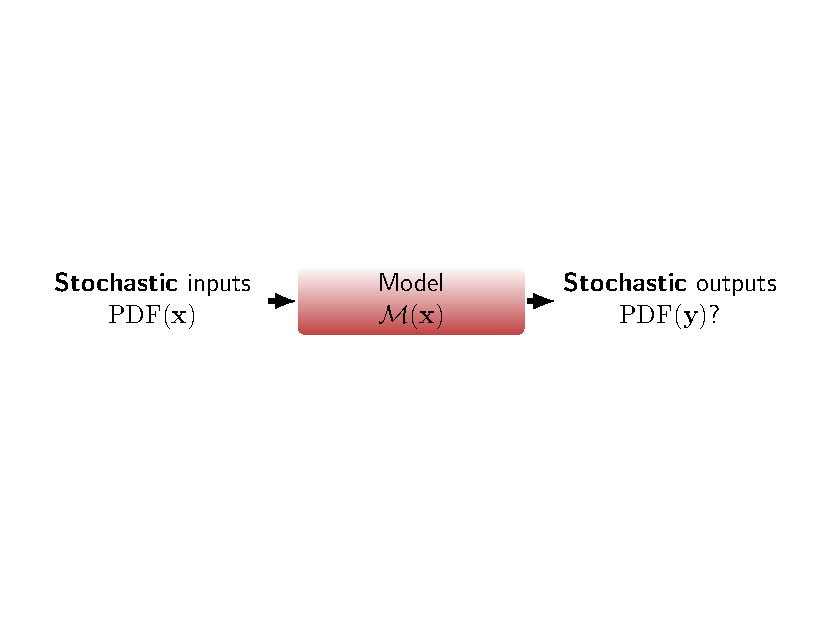
\includegraphics[width=3.5in]{Figures/0_problem_statement.pdf}
\caption{Propagation of uncertainty problem.}
\label{fig_0_propagation}
\end{centering}
\end{figure*}


If a full design load case setup similar to the IEC 61400-1 design cases is used for that purpose, the problem quickly becomes time-consuming as new dynamic simulations would be required for each site. As an example, the number of simulations required to predict within $1\%$ error the lifetime equivalent fatigue loads on a floating wind turbine can reach up to $3,200,000=20^5$ using regular grid-based estimates or in the order of 50,000 using Monte-Carlo simulation \cite{graf2015high}; in this study the inflow conditions (sea/wind fields) are characterized by five stochastic variables. An approach that alleviates these issues is mapping the turbine response to different environmental inputs by means of a fast and accurate surrogate model. Several techniques can be used to predict the behavior of the turbine from a limited set of model evaluations such as: interpolation techniques, response surface techniques, polynomial chaos expansions (PCE), Gaussian process (Kriging) and machine learning techniques. 

A quadratic response surface technique based on a circular central composite design has been used to represent the response of a wind turbine to five environmental input parameters \cite{toft2016assessment}. The probability density function ($\pdf$) of the fatigue load in different components of the NREL 5 MW reference turbine has been studied as function of the $\pdf$ of four inputs: mean wind speed, yaw error, wind shear exponent and wind veer parameter \cite{TallwindReport}. A Kriging surrogate has been used as a function of wind speed and turbulent standard deviation to predict the 50 year extreme loads on a 5 MW wind turbine \cite{abdallah2016influence}. Two different regression-tree wind turbine surrogates have been developed for power production \cite{clifton2013using} and for equivalent fatigue loads \cite{clifton2014effect}; these surrogates use machine learning techniques to predict the output of the turbine as a function of wind speed, turbulence intensity and shear exponent.

Polynomial chaos expansion is a methodology used to efficiently propagate input uncertainties through a non-linear model. This methodology consists in building a polynomial response surface to capture the global dependency of the output as a function of the uncertain inputs. PCE is widely used in the uncertainty quantification field because of its simplicity and fast convergence in comparison to a full Monte-Carlo simulation based on the original model \cite{soize2004physical, le2004uncertainty, choi2004polynomial, berveiller2006stochastic, xiu2005high}. Furthermore, adaptive PCE training algorithms can be used to obtain a sparse surrogate that minimizes the number of terms that have multiple variable dependency, making the surrogates extremely efficient response surface in multiple dimensions  \cite{blatman2011adaptive,pedregosa2011scikit,tibshirani1996regression}. In the case of smooth continuous models with multiple input variables, sparse polynomial chaos expansion methodology is the most efficient technique to build the surrogates in terms of the number of model evaluations required, the number of input dimensions they can handle and the rate of convergence \cite{blatman2011adaptive}.


% ------------------------------------------
%\subsection{Problem statement}
% ------------------------------------------
One of the main difficulties in building a surrogate of an aeroelastic wind turbine model is the fact that the turbulent inflow realization (TIR, i.e. turbulent structures in the flow field) causes variations in the different wind turbine model outputs: such as power, thrust, fatigue and extreme loads in the different components of the turbine. This can be restated as: an aeroelastic wind turbine model has stochastic/non-deterministic outputs. Many studies have analyzed the difficulties of studying fatigue and extreme loads under different turbulent inflow realizations \cite{moriarty2008database, natarajan2012outlier, tibaldi2014investigation, abdallah2016influence, toft2016assessment}. Different TIR activate different dynamics of the structure and have different control system responses; therefore are an important source of uncertainty in the prediction of the outputs of the model \cite{moriarty2008database}. The high variability in the model response to certain turbulent inflow structures has also been shown to be problematic when Monte-Carlo simulation was used to predict lifetime averages of fatigue loads on a floating wind turbine \cite{graf2015high}.


% ------------------------------------------
\subsection{Response to the problem}
% ------------------------------------------
The aim of the present study is to demonstrate a method for building a quick and accurate surrogate of a wind turbine model that predicts the turbine response as a function of multiple stochastic input variables that describe the turbulent inflow on a site ($\vx$). This article proposes the use of two different variable transformations to simplify the polynomial response surface fitting problem, see Figure \ref{fig_2_trans}. The first transformation is the Rosenblatt transformation \cite{rosenblatt1952}, which is used to de-correlate the set of $D$ input variables $\vx = (x_0, x_1, \ldots x_{D-1})$ into a set of independent uniform variables, $\vw = (w_0, w_1, \ldots w_{D-1})$. The second transformation is a logistic transformation, and it is used to enforce constraints on the polynomial surrogates \cite{simard1998transformation}. This transformation enables the use of polynomial surrogates in problems where the output has a minimum and/or maximum value. Without the logistic transformation the polynomial surrogates will present oscillations in the regions where the model has a constant output. The power production of a turbine is an example of a variable with a strict upper constraint corresponding to the rated power.

%, for which the joint probability distribution can be evaluated as $\pdf(\vw) = \prod_{i=0}^{D-1}{\pdf(w_i)}$

\begin{figure*}[h!]
\begin{centering}
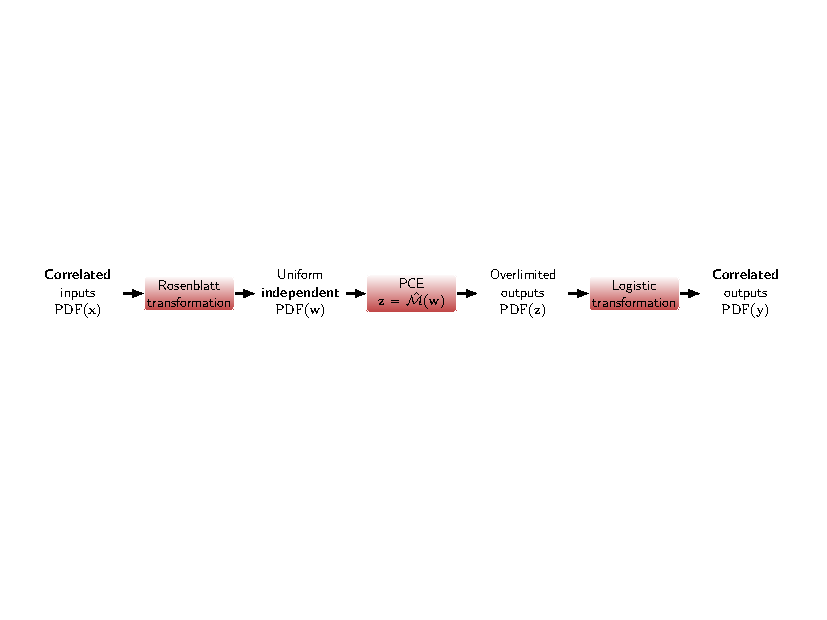
\includegraphics[width=\columnwidth]{Figures/2_transfromation_steps.pdf}
\caption{Transformation of variables to build efficient polynomial response surface.}
\label{fig_2_trans}
\end{centering}
\end{figure*}

The surrogate for the turbine model is a set of two independent polynomial response surfaces that allow to predict the variability caused by different input variable distributions and by different turbulent inflow field realizations (TIR). The distribution of the outputs $\pdf(\vy)$ is predicted through a Monte-Carlo simulation based on the distribution of the input variables $\pdf(\vx)$ using the surrogate model. Similarly, sensitivity analysis is performed using a full Monte-Carlo simulation, from which the input variables can be ranked by importance in explaining the variability in the outputs. 

The two polynomial response surfaces that characterize the distribution of the output at a given input point ($\vx$) are the result of having multiple turbulent inflow fields that have the same statistical parameters. One response surface characterizes the expected output with respect TIR: $\hat{y}_{\expect}(\vx)\approx \expect_{\text{TIR}}(y|\vx)$. The other one describes the standard deviation of the output with respect TIR: $\hat{y}_{\std}(\vx) \approx \sqrt{\variance_{\text{TIR}}(y|\vx)}$. This last response surface can be understood as a model that predicts the uncertainty in the turbine response due to different turbulent structures hitting the turbine. Finally, a sample can be obtained from the normal distribution constructed using the mean and the standard deviation surrogates in order to make a prediction of the variability in the output at a given input point:

%=\std_{\text{TIR}}(y|\vx)

\eq{\hat{y}(\vx) \sim \text{Normal} (\hat{y}_{\expect}(\vx),\, \hat{y}_{\std}(\vx))}{eq_output_distrib}

% ------------------------------------------
\subsection{Article overview}
% ------------------------------------------

A general overview of the PCE methodology in multiple dimensions is presented in section \ref{sec_Methods}. This section describes the Rosenblatt transformation, the design of experiments used to define the training simulation points, the approach used to train sparse polynomial response surfaces and the logistic transformation used to limit the output. In section \ref{sec_Results}, the methodology is then applied to the response of the DTU 10 MW reference wind turbine HAWC2 model \cite{bak2012light} to turbulent inflow fields characterized by four input parameters. The four input parameters are the 10-min averaged hub height wind speed, the turbulent standard deviation of the instantaneous wind speed in the streamwise component, the shear exponent and the yaw misalignment angle. A study of how many independent realizations of the turbulent inflow field are required to achieve a certain error tolerance in the surrogate is presented in the section \ref{subsec_Convergence}. Finally in section \ref{subsec_Final_EX}, the surrogates are used in an example of prediction of the uncertainty in annual energy production and the uncertainty in lifetime equivalent fatigue loads.

\section{Methods}
\label{sec_Methods}

\subsection{1D PCE theory}

% One can define a family of polynomials $\poly_l (x)$ to be used to approximate the output function, where $l$ is the order of the polynomial. In general, if the family of polynomials does not consider any information about the distribution of the input, such as the natural polynomial basis ($1$, $x$, $x^2$, $\dots$), the final approximation of the model is referred to as a polynomial response surface: %\eq{y(x) \approx \sum\limits_{l = 0}^{M} c_l \, \poly_l (x)}{}

Consider a model with a single uncertain input ($x$) and a single output ($y$). PCE consists in defining a polynomial family that is orthogonal with respect the input distribution, $\pdf(x)$. Orthogonal polynomial families with respect the most important distributions are well known, see table \ref{tab_poly}. For details on how to define new polynomial basis to an arbitrary input distributions refer to Gautschi et al \cite{gautschi1994algorithm}.

\begin{table}[h!]
\begin{center}
\resizebox{2.5in}{!}{
\begin{tabular}{lc}
  \hline
  Distribution & Polynomial Family \\
  \hline
  Uniform & Legendre \\
  Normal & Hermite \\
  Exponential & Laguerre \\
  \hline
\end{tabular}}
\caption{Classical orthogonal polynomial families.}
\label{tab_poly}
\end{center}
\end{table}

% It is then required to define an inner product between two arbitrary functions, $f(x)$ and $g(x)$ with respect the probability density function of the input $\pdf(x)$ as:

% \eq{\langle  f, g \rangle  =\int f(x)\,g(x)\, \pdf(x)\,dx}{}

% The polynomial basis ($\phi_{i}$ for polynomial orders $i=0,1,\dots$) is then constructed such that $\phi_{0}=1$ and all the polynomials are orthogonal:

% \eq{\langle  \phi_{l},\phi_{k} \rangle = \delta_{lk} = \begin{cases}
%                         1 \text{ if $l=k$} \\
%                         0 \text{ if $l \neq k$}
%                     \end{cases}}{}

% An important consequence of the orthogonality property is that all the polynomials in the orthogonal basis are orthogonal to the unitary function:

% \eq{\langle 1, \phi_{l} \rangle = 0 \quad \forall l>0 \quad \iff \quad \int \phi_{l}(x)\, \pdf(x)\,dx = 0 \quad \forall l>0}{}

% Note that since the polynomials are of increasing order they can still be used to build a polynomial approximation of the output. i.e. a polynomial response surface. Where, $c_l$ are the coefficients (coordinates) correspondent to each of the elements of the polynomial basis.

The orthogonal polynomials are used to build a polynomial approximation of the output, i.e. a polynomial response surface, see equation \ref{eq_PCE}. Where, $\phi_{l} (x)$ is the $l$ order orthogonal polynomial, $c_l$ is its correspondent coefficient and $M$ represents the truncation order of the PCE.

\eq{y(x) \approx \hat{y}(x) = \sum\limits_{l = 0}^{M} c_l \, \phi_{l} (x)}{eq_PCE}

The orthogonality property makes the PCE an useful approach to propagate uncertainty over a polynomial response surface because the statistical moments of the output can be derived directly from the coefficients:

% \eq{\expect(y) = \int y(x)\, \pdf(x)\,dx  = \langle 1, y \rangle \approx \langle 1, \sum\limits_{l = 0}^{M} c_l \, \phi_{l} \rangle = \sum\limits_{l = 0}^{M} c_l \langle 1, \phi_{l} \rangle = c_{0}}{}

% \eq{\expect(y^2) = \int y^2(x) \pdf(x)\,dx  = \langle y, y \rangle \approx \sum\limits_{l = 0}^{M} \sum\limits_{m = 0}^{M} c_l \, c_{m} \langle \phi_{l}, \phi_{m} \rangle = \sum\limits_{l = 0}^{M} c^2_{l}}{}

% \eq{\variance(y) = \std^2(y) = \expect(y^2) - \expect(y)^2 =  \sum\limits_{l = 1}^{M} c^2_{l}}{}

\eq{\expect(\hat{y}) = c_{0} \quad \quad \variance(\hat{y})=\sum\limits_{l = 1}^{M} c^2_{l}}{}

There are two different approaches to determine the $c_l$ coefficients:

\emph{Semi-Spectral projection} consists in using quadrature rules to approximate the inner product definition of the coefficient, see eq. \ref{eq_projection}. Many quadrature rules exist to approximate the integrals; but all quadrature rules give $N_n$ nodes for model evaluation ($x_i$) and their corresponding weights ($\omega_i$). Gaussian quadrature rules are widely used because they are accurate for smooth function integration with respect a weight function, in this case the $\pdf(x)$, see equation \ref{eq_projection}.

\eq{c_l = \langle  y,  \phi_{l} \rangle  \equiv \int y(x)\, \phi_{l}(x)\, \pdf(x)\,dx \approx \sum_{i=0}^{N_n} \omega_i \, y(x_i) \, \phi_{l}(x_i)}{eq_projection}

\noindent In general, semi-spectral projection is an efficient method for low number of input dimensions, but the number of model evaluations required grows exponentially with the number of dimensions. Additionally, quadrature rules can be unstable for heavy tailed PDFs such as the Weibull distribution \cite{gautschi1994algorithm}.

\emph{Point collocation} consists in fitting the polynomial basis to a small sample of model evaluations. Traditionally, this fit can be done using least squares algorithm, but some other optimization algorithms can be used to obtain PCE approximations that minimize the number of  terms in the surrogate \cite{blatman2011adaptive,pedregosa2011scikit,tibshirani1996regression}. This techniques are explained in the section \ref{sec_LASSO}. In general, point collocation is robust and the advanced optimization algorithms are designed to handle large number of dimensions, to avoid over-fitting and to achieve sparsity in the final surrogate. The present study focuses only in the point collocation techniques since the number of model evaluations required to fit a multiple dimensional PCE is smaller \cite{blatman2011adaptive} than in other methods.

\subsection{Rosenblatt transformation}

To build the PCE of a model with multiple correlated inputs ($\vx$), it is required to initially transform the correlated input space into an uncorrelated space ($\vw=R^{-1}(\vx)$). In this article, the Rosenblatt transformation is used because the input distribution of the turbulent inflow field parameters are usually defined in a sequence of conditional relationships. Refer to Dimitrov et al \cite{dimitrov2015model} and Graf et al \cite{graf2015high} for examples of such distributions used for offshore and floating wind turbine fatigue and extreme load analysis.

The sequential dependency means that the distribution of each of the input variables is given by a parametric $\pdf_i$, whose parameters $\vp_i$ are themselves functions of the previous input variables:

\eq{X_i \sim \pdf_{i}(x_i|\vp_i = \vp_i(x_0,x_1,\dots,x_{i-1}))}{}

The Rosenblatt transformation consists in using the conditional cumulative distribution function of each individual variable, $\cdf_i$, in sequence to transform the variable into an uncorrelated uniform variable \cite{rosenblatt1952}:

\eq{w_i = R^{-1}(x_i) = \cdf_{i}(x_i|\vp_i = \vp_i(x_0,x_1,\dots,x_{i-1}))}{eq_Rosen}

\noindent or to use the inverse $\cdf^{-1}_i$ to transform the uniform variable into the corresponding input:

\eq{x_i = R(w_i) = \cdf^{-1}_{i}(w_i|\vp_i = \vp_i(x_0,x_1,\dots,x_{i-1}))}{eq_Rosen}

Since all the variables are transformed into uncorrelated unitary uniform variables then the PCE only requires the use of the Legendre polynomials: $y(\vx) = y(R(\vw)) \approx \hat{y}(\vw)$. 

%See appendix \ref{app_leg_poly} for the equations of the Legendre polynomials for an unitary uniform variable.

%% The Rosenblatt transformation should be quite trivial - if it is necessary to shorten the paper, this is something that can be shortened significantly.

% An example of the Rosenblatt transformation is shown in figure \ref{fig_rosen}.

% \begin{figure}[h!]
% \begin{centering}
% 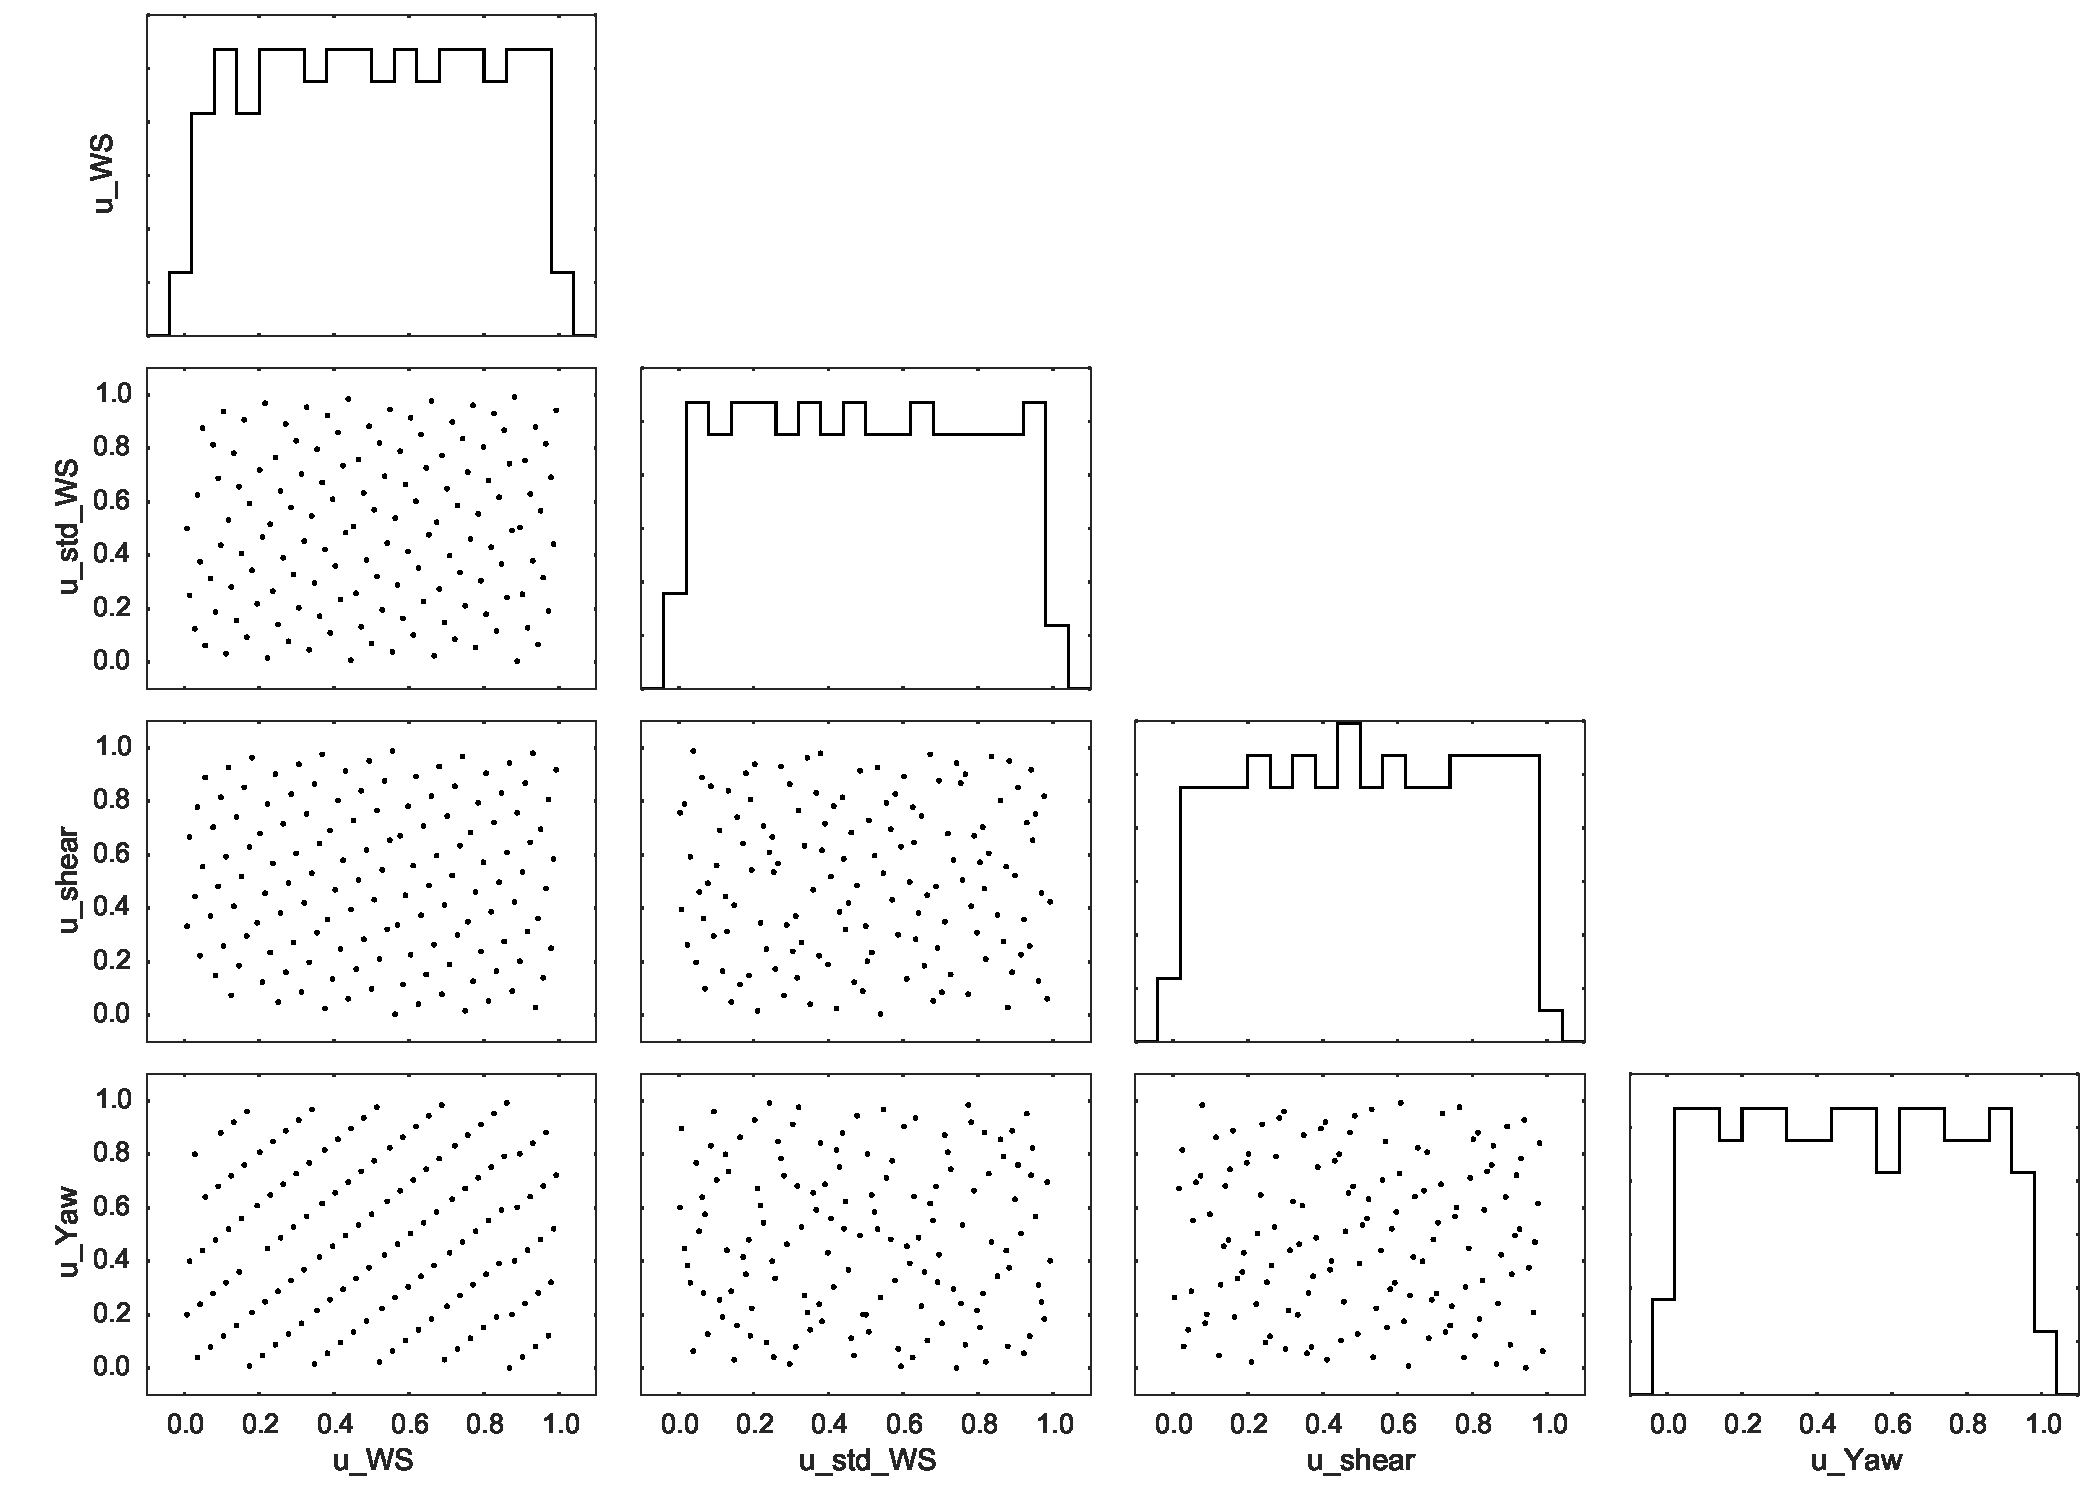
\includegraphics[width=0.48\columnwidth]{Figures/PCE_train_x_Unif.pdf}
% 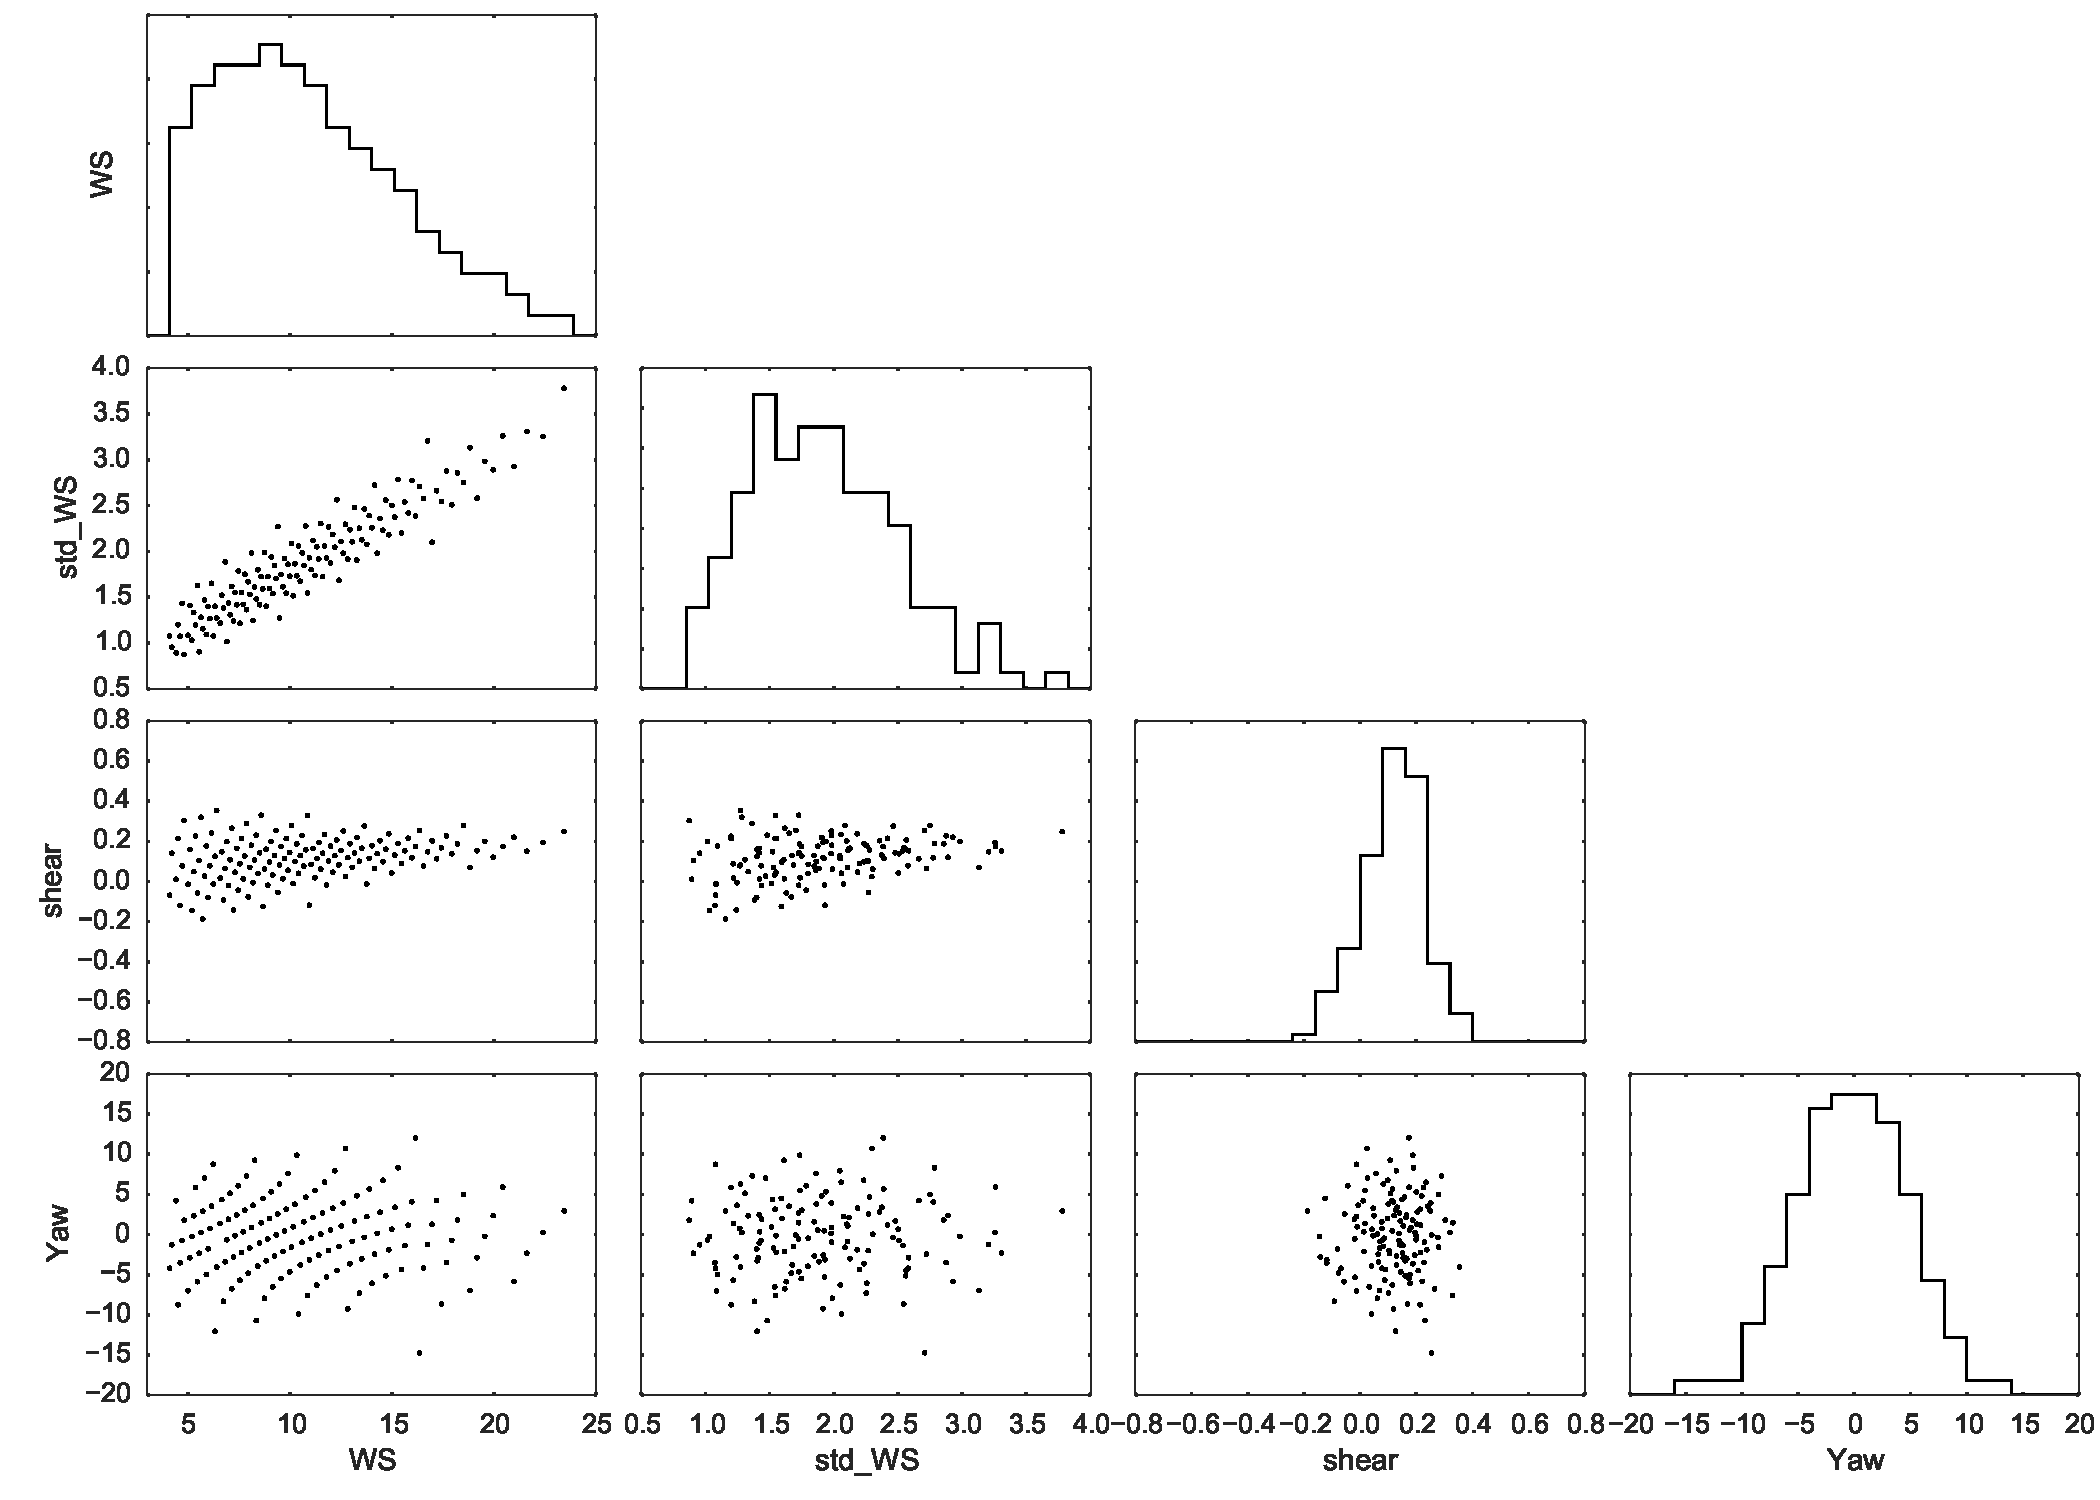
\includegraphics[width=0.48\columnwidth]{Figures/PCE_train_x.pdf}
% \caption{(Left) Sample in the uncorrelated uniform space $\pdf(\vw)$. (Right) Same sample transformed into the correlated input space $\pdf(\vx)$.}
% \label{fig_rosen}
% \end{centering}
% \end{figure}

\subsection{Multi-dimensional PCE}

A D-dimensional polynomial is constructed as the sum of the product between individual one dimensional polynomials for each of the $D$ uniform input variables, $\vw=[w_0,\dots,w_{D-1}]$. The $D$-dimensional surrogate is written using a set of multiple indexes $\multind \subset \mathbb{N}^D$. An element $J\in \multind$ contains the order of the polynomial in each dimension: $J = [l_0, \dots, l_{D-1}]$. Additionally, the multiple indexes are enumerated, $J \leftrightarrow j \in \mathbb{N}$. A surrogate that contains $N_c$ terms can be written as:

\eq{y(\vx) = y(R(\vw)) \approx \sum\limits_{j=0}^{N_c-1} c_{j} \, \mpoly_{j} (\vw)}{}

\noindent where an element in the multidimensional polynomial basis is given as:

\eq{\mpoly_{j} (\vw) =  \phi_{l_0}(w_0) \times \dots \times \phi_{l_{D-1}}(w_{D-1})}{}

% An example of a 3-dimensional polynomial response surface with 4 terms is given in table \ref{tab_MD_example}. In this example the multi-dimensional polynomial is given in eq. \ref{eq_example_yhat}. This equation can be evaluated using the Legendre polynomials, $\phi_{l}(w)$. Note that $\phi_{0}(w)=1$.

% \begin{table}[h!]
% \begin{centering}
% \resizebox{0.25\linewidth}{!}{
% \begin{tabular}{|c|ccc|c|}
%     \hline
%     $j$ &  $l_0$ &  $l_1$ &  $l_2$ &  $c_j$ \\
%     \hline
%     0  &   0 &   0 &   0 &    0.5 \\
%     1  &   1 &   0 &   0 &    7.5 \\
%     2  &   2 &   2 &   0 &   -1.4 \\
%     3  &   3 &   1 &   2 &   21.1 \\
%     \hline
% \end{tabular}}
% \caption{Example of the notation of a 3-dimensional polynomial response surface.}
% \label{tab_MD_example}
% \end{centering}
% \end{table}%

% \eq{\hat{y}(\vw)=0.5 +  7.5 \,\phi_{1}(w_0)  -1.4 \,\phi_{2}(w_0) \,\phi_{2}(w_1) +  21.1 \,\phi_{3}(w_0) \,\phi_{1}(w_1) \,\phi_{2}(w_2)}{eq_example_yhat}

\subsection{Training point selection}

The Rosenblatt transformation enables the use of multiple variance reduction Monte-Carlo sampling techniques to define the training points of a surrogate \cite{feinberg2015chaospy}. Latin hypercube sampling \cite{mckay2000comparison}, Sobol sequence \cite{sobol1967distribution} and Hammersley sequence \cite{hammersley1960monte} are some examples of such techniques. These techniques are designed to sample from the unitary hypercube of $D$ dimensions, i.e. the uniform distributed variables: $\vw_i \sim \pdf(\vw)$. Finally, the Rosenblatt transformation is used to transform each realization in the uniform sample into the correlated input space, $\vx_i = R(\vw_i) \sim \pdf(\vx)$.

The number of unknown coefficients $c_j$ in a D-dimensional PCE depends of the total polynomial order of the PCE. The total order is defined as the maximum sum of the one dimensional orders. If the PCE is truncated to a total order $M$ then the number of unknown coefficients is given by the following combination:

\eq{N_c = {M + D \choose M} = \frac{(M+D)!}{M! \, D!} }{eq_mod_eval}

The number of model evaluations should be between 2 or 3 times the number of unknowns in order to have extra data to test the accuracy of the surrogate and to implement strategies to avoid over-fitting \cite{blatman2011adaptive}. Note that the maximum order is only used to estimate the number of model evaluations. Advanced regression techniques allow to explore higher order terms \cite{tibshirani1996regression, blatman2011adaptive}. The maximum order $M$ can be increased in order to achieve higher accuracy surrogates but at the cost of having more model evaluations and the requirement of assuring that there is not over-fitting.

\subsection{Point collocation and the LASSO problem}
\label{sec_LASSO}

The least absolute shrinkage and selection operator (LASSO) problem is a modified least squares optimization problem that adds a term that penalizes the amount of active terms in the surrogate (terms with non zero coefficients). LASSO is used to achieve sparsity and to avoid over fitting in the surrogate. Additionally, the number of model evaluations required for solving the LASSO problem is smaller in comparison to a least squares regression that has the same maximum polynomial order $M$ \cite{blatman2011adaptive}.

A LASSO problem can be described as finding the set of coefficients $c_j$ that minimizes the sum of squared errors plus the sum of the absolute values of all coefficients ($\ell_1$ norm regularization term) \cite{tibshirani1996regression}:

%\min_\vc ||\vc \boldsymbol{\Phi} - \text{\textbf{y}}||^2_2 + \alpha ||\vc||_1 =

\eq{\min_{c_j} \quad \sum_{i=0}^{N-1} \left[ \sum_{j=0}^{N_c-1} c_j \mpoly_j(\vw_i) - y(\vx_i) \right]^2 + \alpha \sum_{j=0}^{N_c-1} |c_j|}{}

\noindent where the number of model/surrogate evaluation points $N$ is fixed. Note that the input and surrogate evaluation points are related by the Rosenblatt transformation $\vx_i=R(\vw_i)$. The maximum number of possible terms of the surrogate $N_c$ is also fixed by selecting a maximum total multi-dimensional polynomial order.

The regularization coefficient $\alpha$ controls the amount of active terms in the final solution. Smaller values allow to have more active terms while larger values will prefer final surrogates with few active terms. A sparse surrogate has the advantage of making the evaluation of the multi-dimensional surrogate faster in comparison to the full least squares solution; this advantage becomes critical in high number of input dimensions.

There are two algorithms widely used to solve the LASSO problem: coordinate descent \cite{tibshirani1996regression} and least angle regression (LAR) \cite{blatman2011adaptive}. Coordinate decent is used in the present work because it tends to be more stable for high dimensional problems \cite{pedregosa2011scikit}. The reason for this is that coordinate descent operates on a given regularization coefficient instead of exploring the full space of $\alpha$'s as in LAR algorithm.

% \subsection{k-Fold cross-validation for LASSO regularization coefficient selection}

Cross-validation is used to select the regularization coefficient $\alpha$ that minimizes over fitting of the data. A k-fold cross-validation consists in splitting the dataset into k groups of data. All the points in k-1 groups are used for training and the remaining group is used for cross-validation. This means that the surrogate fitted using k-1 groups is used to predict the output in each of the elements of the remaining group. The mean squared error of the prediction of the surrogate is then computed. This process is repeated leaving out each individual fold and for multiple regularization parameters. The regularization parameter that gives the lowest mean cross-validation mean squared errors is then selected to train the whole dataset. This translates as selecting the sparse model that performs the best by predicting missing data, i.e. that has less over-fitting. 

% Figure \ref{fig_overfitting} shows an example in which an over fitted model has a larger cross validation prediction error than a sparse surrogate.

% \begin{figure}[h!]
% \begin{centering}
% 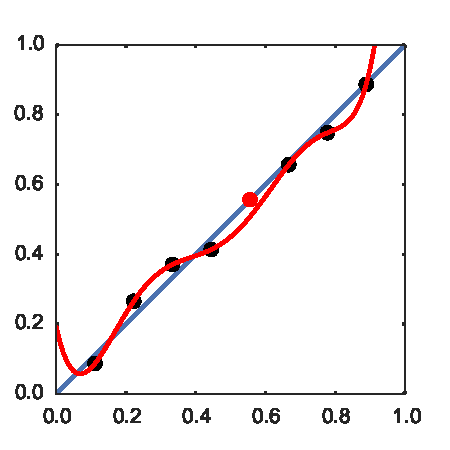
\includegraphics[width=0.3\columnwidth]{Figures/overfitting_CV.pdf}
% 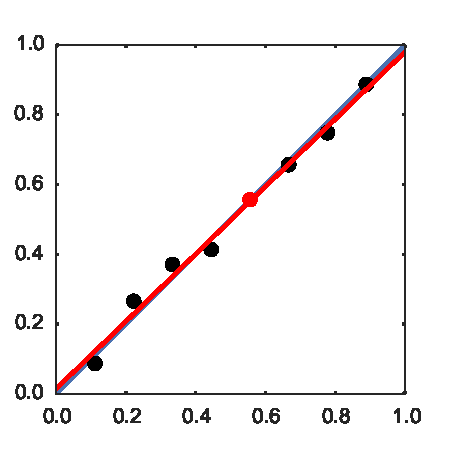
\includegraphics[width=0.3\columnwidth]{Figures/overfitting_solved_CV.pdf}
% \caption{Simple example of over fitting and cross validation. The red point is only used for cross validation. (Left) Over fitted surrogate. (Right) Optimal surrogate.}
% \label{fig_overfitting}
% \end{centering}
% \end{figure}


\subsection{Logistic transformation}

A logistic transformation is applied to an output of the model in order to avoid oscillations in the regions where the model is constant. In practice this transformation is used to impose strict restrictions on the polynomial surrogates. The logistic transformation uses the logit function:

\eq{L(p)= \ln \left( \frac{p}{1-p} \right) }{}

\noindent and its inverse, the logistic function:

\eq{L^{-1}(q) = \frac{1}{1+e^{-q}}}{}

The transformation consists in applying the logit function to the model output at the training points $y_i=y(\vx_i)$ to define the training points in the possibly over-shooting variable space $z_i$ \cite{simard1998transformation}, see equation \ref{eq_logit}. The surrogates are then fitted to the $z_i$ outputs.

\eq{z_i = L(a_1\,y_i+a_0)}{eq_logit}

Finally, each time the surrogate is evaluated, the prediction of the surrogate $\hat{z}$ is transformed back to the original output space $\hat{y}$, see equation \ref{eq_logistic}. The constants of the transformation ($a_0$ and $a_1$) are calibrated in order to impose the constrains of the output and to avoid numerical instabilities that are inherent to the logit function.

\eq{\hat{y} = \frac{L^{-1}(\hat{z}) - a_0}{a_1} }{eq_logistic}


\subsection{Global sensitivity analysis}

Global sensitivity analysis (SA) is a methodology to determine how important each input is to explain the variance of the output. SA can be obtained with a Sobol variance decomposition \cite{sobol2001global}. In this technique, the variance of the output is explained into the different terms of variance of each of the inputs, in a process similar to the analysis of the variance of experiments (ANOVA) \cite{maxwell2004designing}. Total effect Sobol indices are widely used as measures of how much of the variance of a given output is explained by the variance of an input, including possible interactions with other variables. This method is the most recognized method for global sensitivity analysis because it accounts for non-linear dependencies and for interactions between variables \cite{saltelli2010variance}.

Variance decomposition can be expressed as the sum of the variance of the marginal expected value of a subset of input variables, see eq. \ref{eq_var_dec}. Note that this decomposition is not an infinite series expansion, it is truncated to the maximum number of variable interactions.

\eq{
\begin{aligned}
\variance(y) = \sum\limits_{k=0}^{D-1} \variance_k & + \sum\limits_{k=0}^{D-1} \sum\limits_{l>k}^{D-1} \variance_{kl} + \sum\limits_{k=0}^{D-1} \sum\limits_{l>k}^{D-1} \sum\limits_{m>l}^{D-1} \variance_{klm} + \dots + \variance_{0\dots D-1}\\
\variance_{k} & = \variance \left( \expect_{\forall n \neq k}\left( \model(\vx | x_k) \right) \right)\\
\variance_{kl} & = \variance \left( \expect_{\forall n \neq k,l}\left( \model(\vx | x_k, x_l) \right) \right) \\
\variance_{klm} & = \variance \left( \expect_{\forall n \neq k,l,m}\left( \model(\vx | x_k, x_l, x_m) \right) \right)
\end{aligned}
}{eq_var_dec}

The global sensitivity measure is defined by normalizing eq. \ref{eq_var_dec} with the total variance of the output $\variance(y)$. From this normalization one can define the Sobol index of a given degree of interaction between input variables as:

\eq{ S_{k} = \frac{\variance_{k}}{\variance(y)} \quad \quad S_{kl} = \frac{\variance_{kl}}{\variance(y)}  \quad \quad S_{klm} = \frac{\variance_{klm}}{\variance(y)} \quad \dots}{}

The total effect Sobol index of an input variable $x_i$ is then the sum of all the Sobol indices that include the variable in any interaction:

\eq{ S_{\text{total}\,x_i} = S_{i} + \sum\limits_{\substack{k=0\\k \neq i}}^{D-1} S_{ik} + \dots}{}

%The Sobol indices can be understood as, the fraction reduction in the variance of the output that could be achieved if the variance in the $i$-th variable could be suppressed.
The sensitivity analysis of the response of the turbine should consider the effect of having different turbulent inflow realizations. The turbulent inflow is modeled with the two independent PCE for the local mean and local standard deviation. Therefore, even though the Sobol indexes could be computed directly from the PCE coefficients, see Sudret et al \cite{sudret2008global}, they would not include the effect of the turbulence inflow realization. To solve this limitation, the approximate method proposed in Saltelli et. al \cite{saltelli2010variance} is used to compute the total effect Sobol indexes. This approach estimates the total effect Sobol indexes from a large Monte-Carlo simulation.

% Furthermore, the total effect Sobol's indexes can also be calculated using only the coefficients of the PCE \cite{sudret2008global}:

% \eq{S_{\text{total}\,x_k} = \frac{\sum\limits_{\substack{J \in \multind \\ l_k>0}} c_{j}^2}{\sum\limits_{\substack{J \in \multind \\ J\neq[0,0,\dots,0]}} c_{j}^2} }{}

\section{Results}
\label{sec_Results}

\subsection{Implementation}

Several open source implementations of PCE methods are available such as: Chaospy \cite{feinberg2015chaospy}, Dakota \cite{eldred2007dakota}, UQLab \cite{marelli2014uqlab} and OpenTurns \cite{andrianov2007open}. In the present work we use Chaospy because of its implementation of the Rosenblatt transformation. Additionally, the present work uses the  LASSO problem solvers \cite{tibshirani1996regression} and the cross-validation capabilities available in the open source library Scikit-learn \cite{pedregosa2011scikit}. These capabilities are used inside of Chaospy for general users and are used externally in the present study to gain control over the different stages of the cross-validation.

\subsection{Case description}

The model consists of the DTU 10 MW reference wind turbine HAWC2 model \cite{larsen20072, bak2012light} with Mann turbulent inflow generation \cite{Mann1998}. The turbulent inflow conditions are defined using the four variables described in table \ref{tab_ins}.

\begin{table}[!h]
\begin{centering}
\resizebox{5in}{!}{
\begin{tabular}{lcccc}
    \hline
    Input & Variable & Distribution & \multicolumn{2}{c}{Parameters} \\
    \hline
    \\[-0.6em]
    10-min mean hub height & $x_0=\ws$ & Rayleigh & \multicolumn{2}{c}{$\expect(\ws) = 10$ m/s}\\
    wind speed  & & & &\\
    \\[-0.6em]
    Std. of the inst. wind speed & & & &\\
    in the streamwise direction & $x_1=\stdws$ & Lognormal & $\mu_{\stdws}(\ws)$ & $\sigma_{\stdws}(\ws)$ \\
    during the 10-min simulation & & & &\\
    \\[-0.6em]
    10-min mean shear exponent & $x_2=\shear$ & Normal & $\mu_{\shear}(\ws)$ & $\sigma_{\shear}(\ws)$ \\
    \\[-0.6em]
    10-min mean yaw miss-align. & $x_3=\yaw$ & Normal & $\mu_{\yaw}=0$ & $\sigma_{\yaw}= 5$ deg. \\
    \hline
\end{tabular}}
\caption{Wind turbine model inputs.}
\label{tab_ins}
\end{centering}
\end{table}

The dependency between $\ws$ and $\stdws$ is defined in the Normal Turbulence Model described in the IEC 61400-1 \cite{international2005iec}. The present case uses a reference ambient turbulence intensity of a site Class 1A:  $\text{TI}_{\text{ref}} = 0.16$. This dependency is given by the local statistical moments of $\stdws$ as:

\eq{
\begin{split}
\expect(\stdws|\ws) & = \text{TI}_{\text{ref}} \, (0.75 \ws + 3.8) \\
\variance(\stdws|\ws) &= (1.4 \,\text{TI}_{\text{ref}} )^2 \\
\end{split}
}{}

\noindent %which translates into a dependency of the local Lognormal distribution parameters of $\stdws$ as:
%
%\eq{
%\begin{split}
%\sigma_{\stdws} &= \left( \ln\left( \frac{\variance(\stdws|\ws)}{\expect^2(\stdws|\ws)} + 1 \right) \right)^{1/2} = \left(\ln \left( \frac{1.4^2}{(0.75 \ws + 3.8)^2} + 1 \right) \right)^{1/2}\\
%\mu_{\stdws} &= \ln \left(\expect(\stdws|\ws)\right) - \frac{\sigma_{\stdws}^2}{2} = \ln \left( \text{TI}_{\text{ref}} \, (0.75 \ws + 3.8) \right) - \frac{\sigma_{\stdws}^2}{2}
%\end{split}
%}{eq_std}

%% I think translating from expected value and variance to the log-normal distribution parameters is trivial, we can leave it out

The correlation between $\shear$ and $\ws$ is based on the simplified joint distribution defined by Dimitrov et al \cite{dimitrov2015model}:

\eq{\begin{split}
\mu_{\shear} & = 0.088 (\ln(\ws) - 1) \\
\sigma_{\shear} &= 1/\ws
\end{split}
}{eq_shear}


Seven different model outputs are considered ($\vy$), see table \ref{tab_outs}. The damage equivalent fatigue loads (EFL) are computed using a rainflow counting algorithm to determine the number of load cycles $n_i$  with their corresponding load range $S_i$  in the 10-min time series of turbine response. The EFL is then weighted using different materials' W{\"o}hler exponent $m$, see equation \ref{eq_EFL} by Miner et al \cite{miner1945cumulative}. For obtaining 1Hz-equivalent fatigue loads based on 10 minute reference periods, the reference number of load cycles used is $N_{\text{ref}}=600$.

\eq{S_{\text{eq}} = \left( \frac{\sum n_i S_i^m}{N_{\text{ref}}} \right)^\frac{1}{m}}{eq_EFL}

\begin{table}[!h]
\begin{centering}
\resizebox{4in}{!}{
\begin{tabular}{lcc}
    \hline
    Output & $m$ & Variable \\
    \hline
    10 minute mean power production & - & $P$ \\
    10 minute mean thrust coefficient & - & $CT$ \\
    EFL blade root flapwise bending moment & 12 & BRF \\
    EFL tower bottom fore-aft bending moment & 4 & TBF  \\
    EFL tower bottom sidewise bending moment & 4 & TBS \\
    EFL tower top tilt bending moment & 4 & TTT \\
    EFL tower top yaw bending moment & 4 & TTY \\
    \hline
\end{tabular}}
\caption{Wind turbine model outputs.}
\label{tab_outs}
\end{centering}
\end{table}

\subsection{Training points}

In this study, the number of model evaluations are set to be $N=2\,N_c$, and the maximum order of the polynomial is expected to be $M=4$. This leads to a number of model evaluations of 140 for a 4-dimensional case, see equation \ref{eq_mod_eval}. %% A small comment: I tested some other low-discrepancy series available in Matlab (Sobol, Halton), and to me the Halton sequence actually looks interesting - it may have an advantage over the Hammersley because in higher dimensions the Hammersley points tend to start looking grouped - but this doesn't seem to be the case with Halton sequence points. 
A Hammersley sequence \cite{hammersley1960monte} is preferred over other variance reduction methods to generate the training sample in the uniform space as it is a sequence that can be extended to contain larger sample size without changing the previous points \cite{feinberg2015chaospy,hosder2007efficient}. The uniform sample is then transformed into the physical variables using the Rossenblat transformation. A similar approach is used to generate the input sample for a Monte-Carlo simulation; the only difference is the size of the sample which in this study is taken to be 80000. The training input sample is shown in figure \ref{fig_PCE_train_x_full} as well as a the inputs sample for the Monte-Carlo simulation. It can be observed that the training points are more densely distributed in the regions of higher probability of the inputs. This means that the surrogate is better trained in the most likely regions of the input space.  100 different turbulent inflow realizations are generated using the Mann model for each input point, for which the mean and standard deviation of the outputs are obtained. This number is selected to allow for testing in the accuracy of the prediction of the surrogates when they are trained using a reduced number of TIR. This makes the full training sample size of $140 \times 100$ HAWC2 10 minutes simulations.

\begin{figure*}[h!]
\begin{centering}
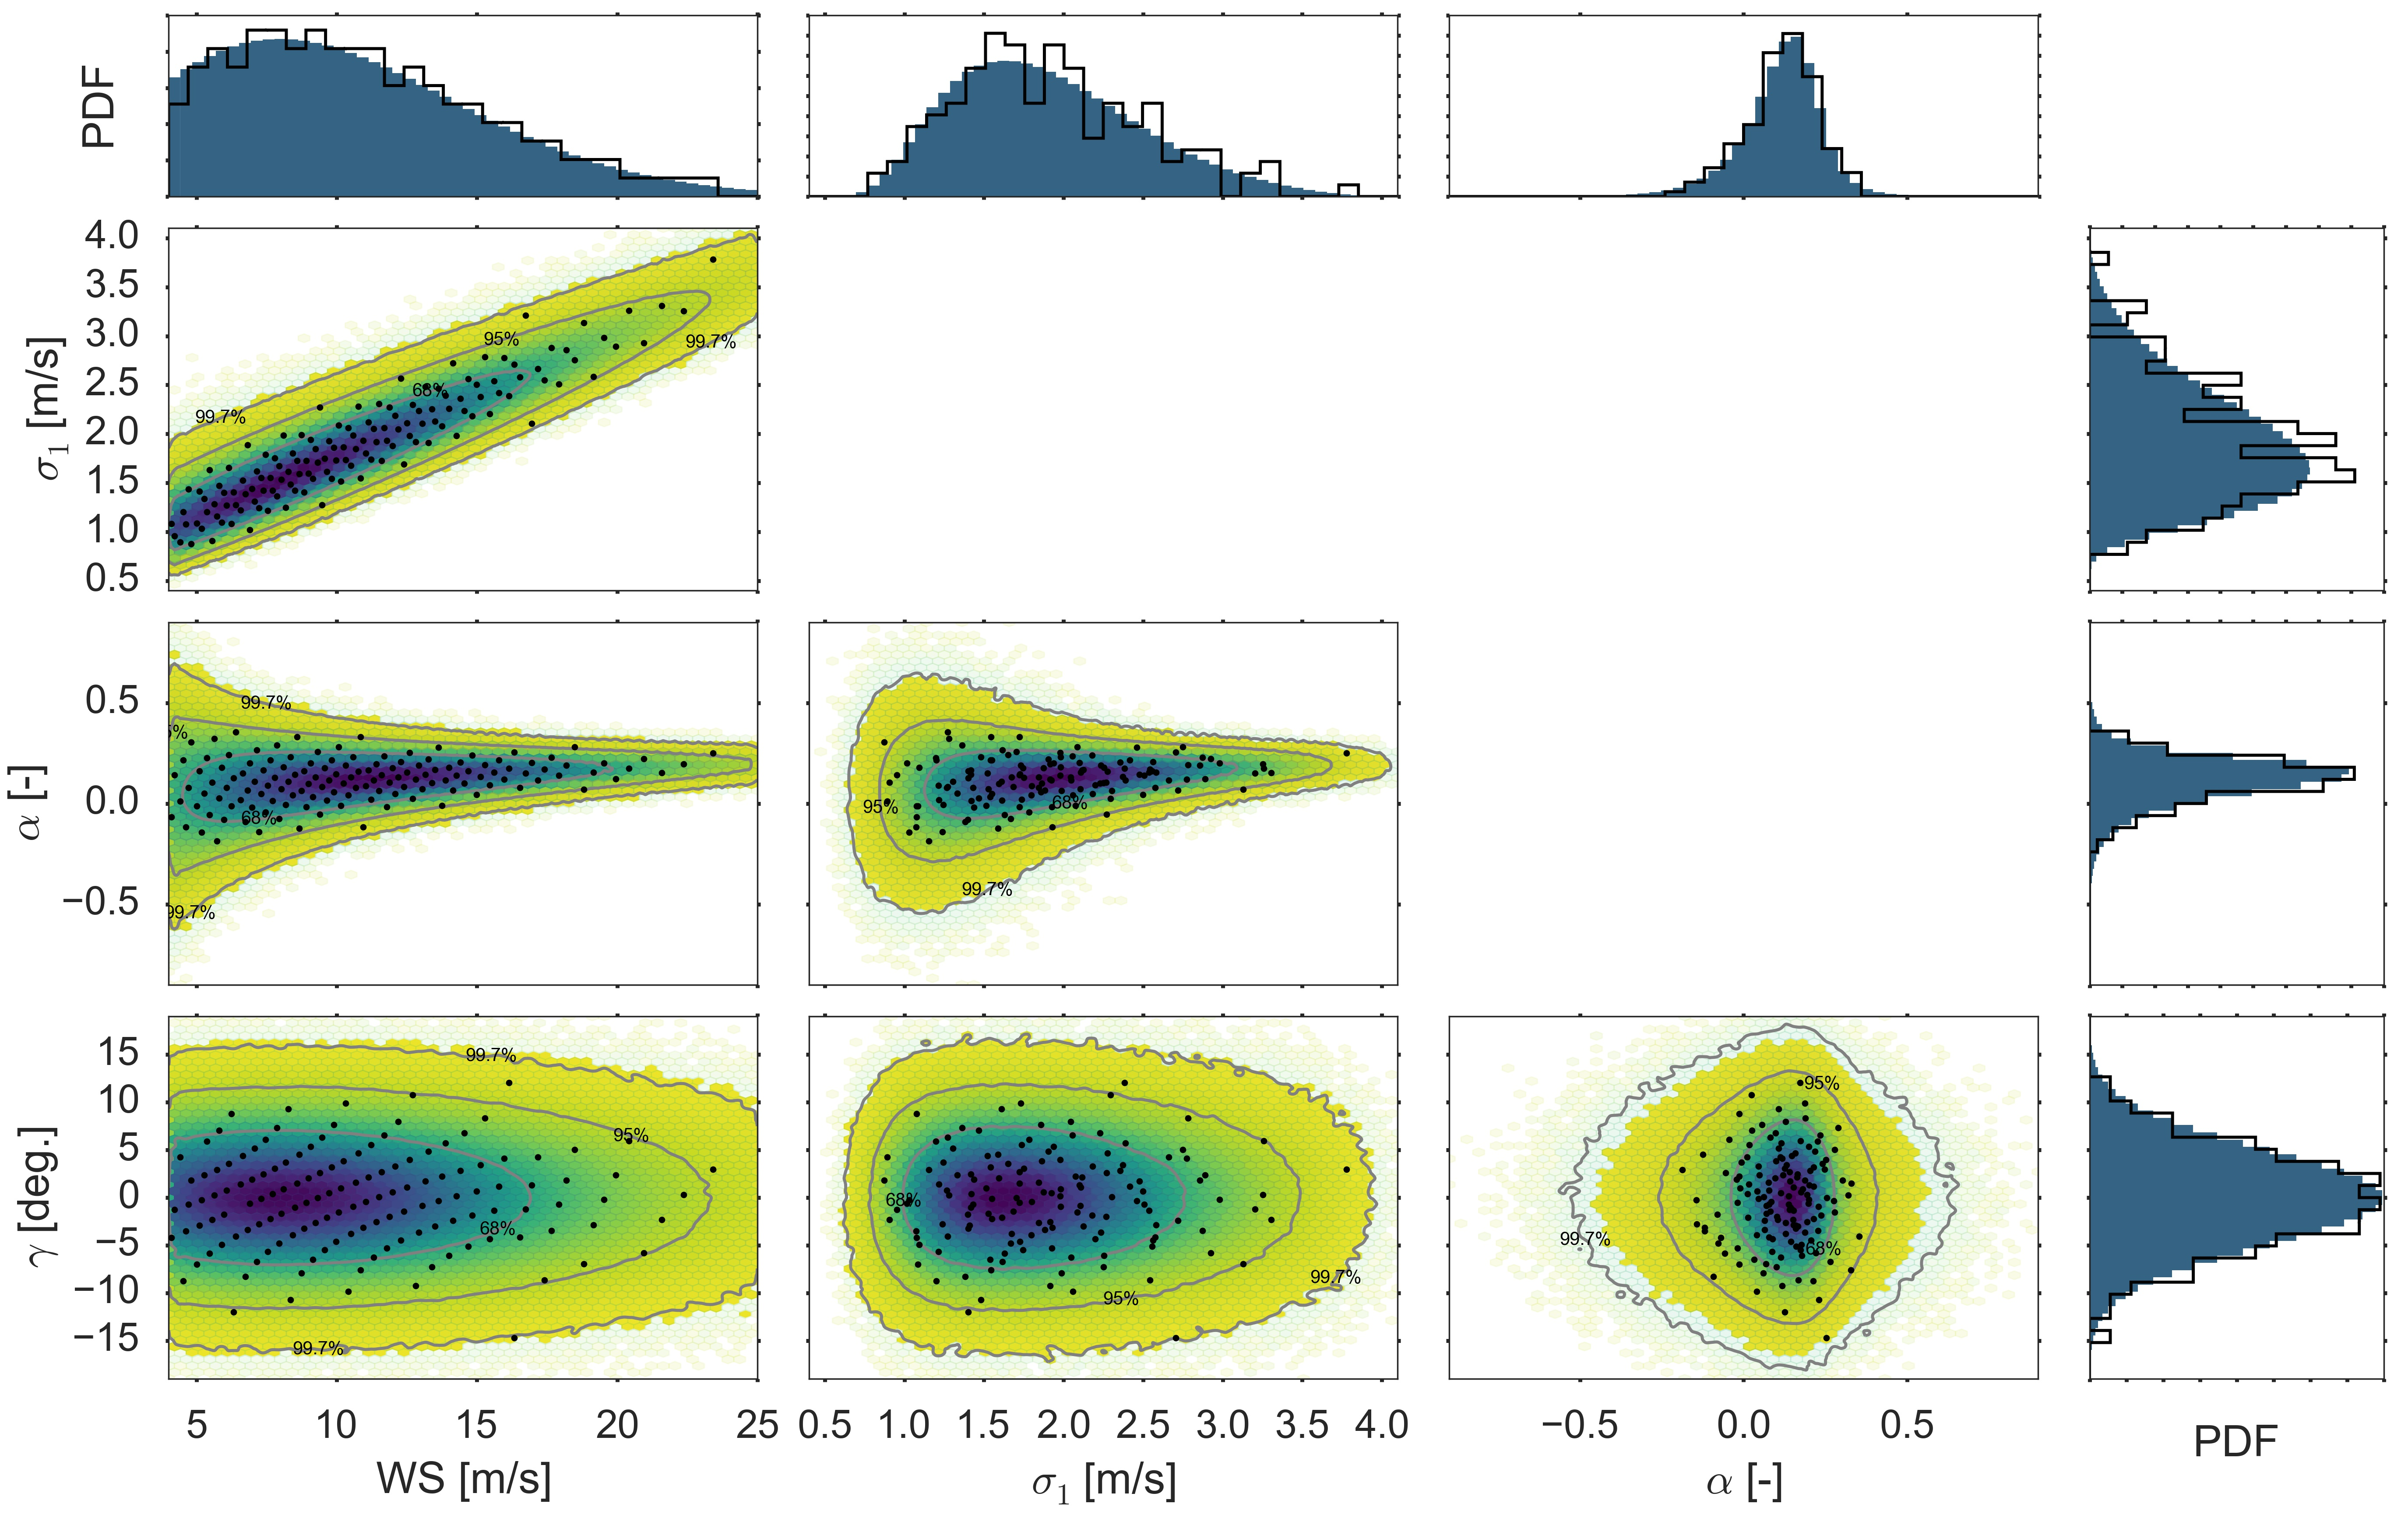
\includegraphics[width=\linewidth]{Figures/PCE_train_x_full.jpg}
\caption{(Black points) Training dataset in the inputs: 140 Hammersley sequence sample of input joint distribution. (Histogram colored hex-bins) 80000 Hammersley sequence sample Monte-Carlo sample.}
\label{fig_PCE_train_x_full}
\end{centering}
\end{figure*}

\subsection{Example of PCE surrogates for individual statistical moments}

Some examples of the surrogates for $\vy_{\expect}$ and $\vy_{\std}$ \footnote{$P_{\std}$ represents the standard deviation of 100 different realizations of the 10-min averaged power; this variable should not be confused with the standard deviation of the instantaneous power during the 10 minutes of simulation.} are shown in figures \ref{fig_y_hat_E_V} and \ref{fig_y_hat_E_V2}. In general, the surrogates accurately capture the global behavior of the model with respect to the 4 input variables. The surrogates of the local standard deviations present larger errors, although the errors are small in comparison to the overall magnitude of the output. These local errors cause an inability to fully capture the overall distribution of the local standard deviations, see the plots in the fifth column in figures \ref{fig_y_hat_E_V} and \ref{fig_y_hat_E_V2}. The distribution of the errors of the surrogate and its impact in the final prediction are quantified in section \ref{subsec_Convergence}. These errors can be reduced up to a tolerance level selected by the user by adding more training points (input points with their turbulent inflow realizations).

\begin{figure*}[h!]
\begin{centering}
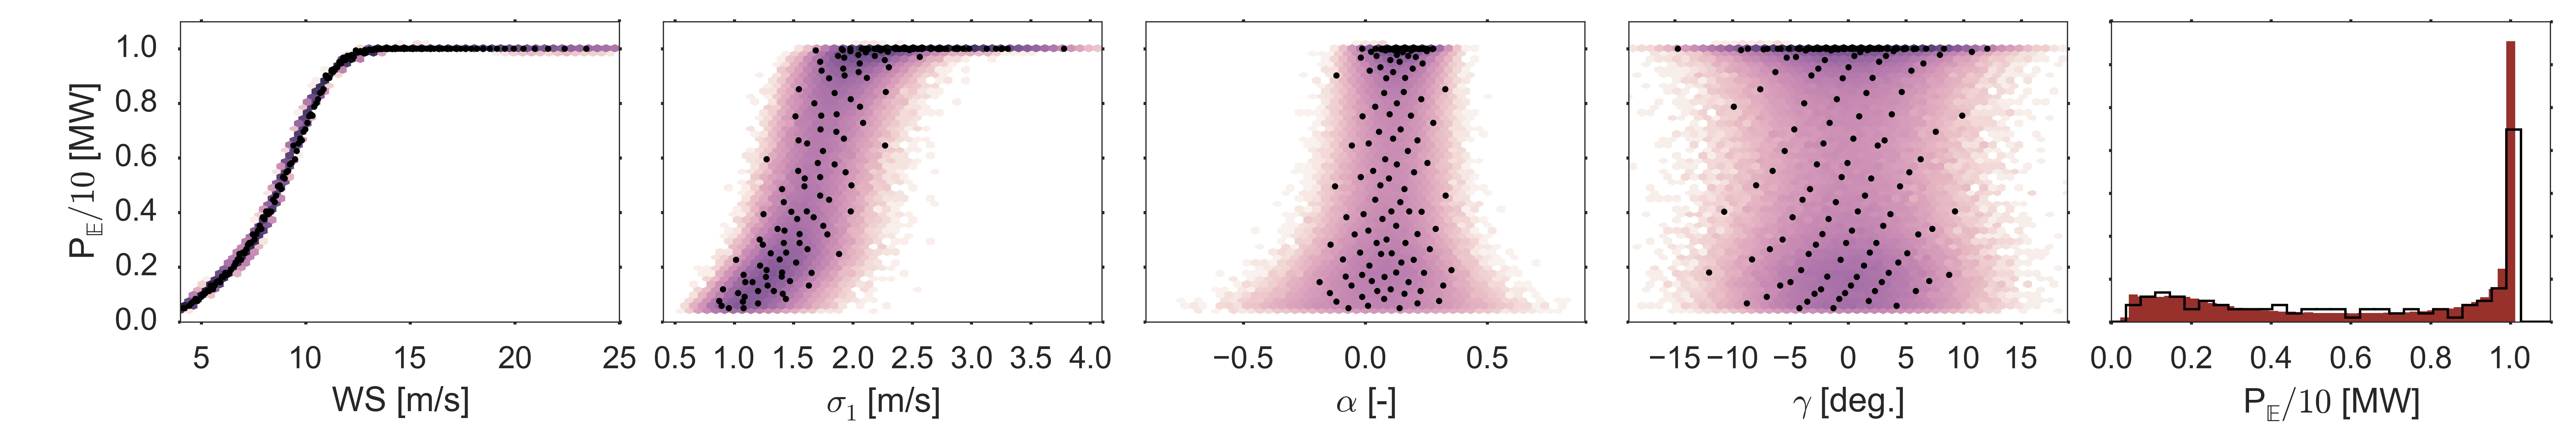
\includegraphics[width=\linewidth]{Figures/Surrgotes_20-fold/P_E_MC_PCE_last_row.jpg} \\
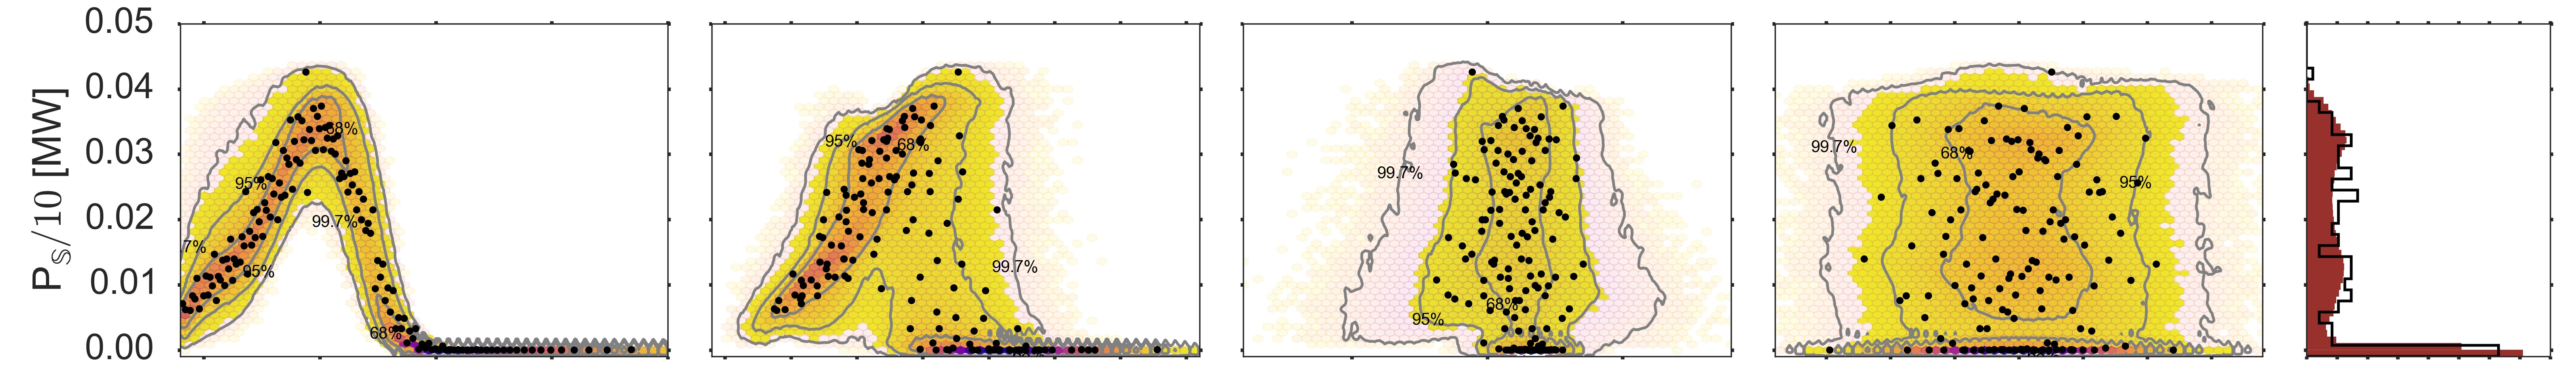
\includegraphics[width=\linewidth]{Figures/Surrgotes_20-fold/P_S_MC_PCE_last_row.jpg} \\
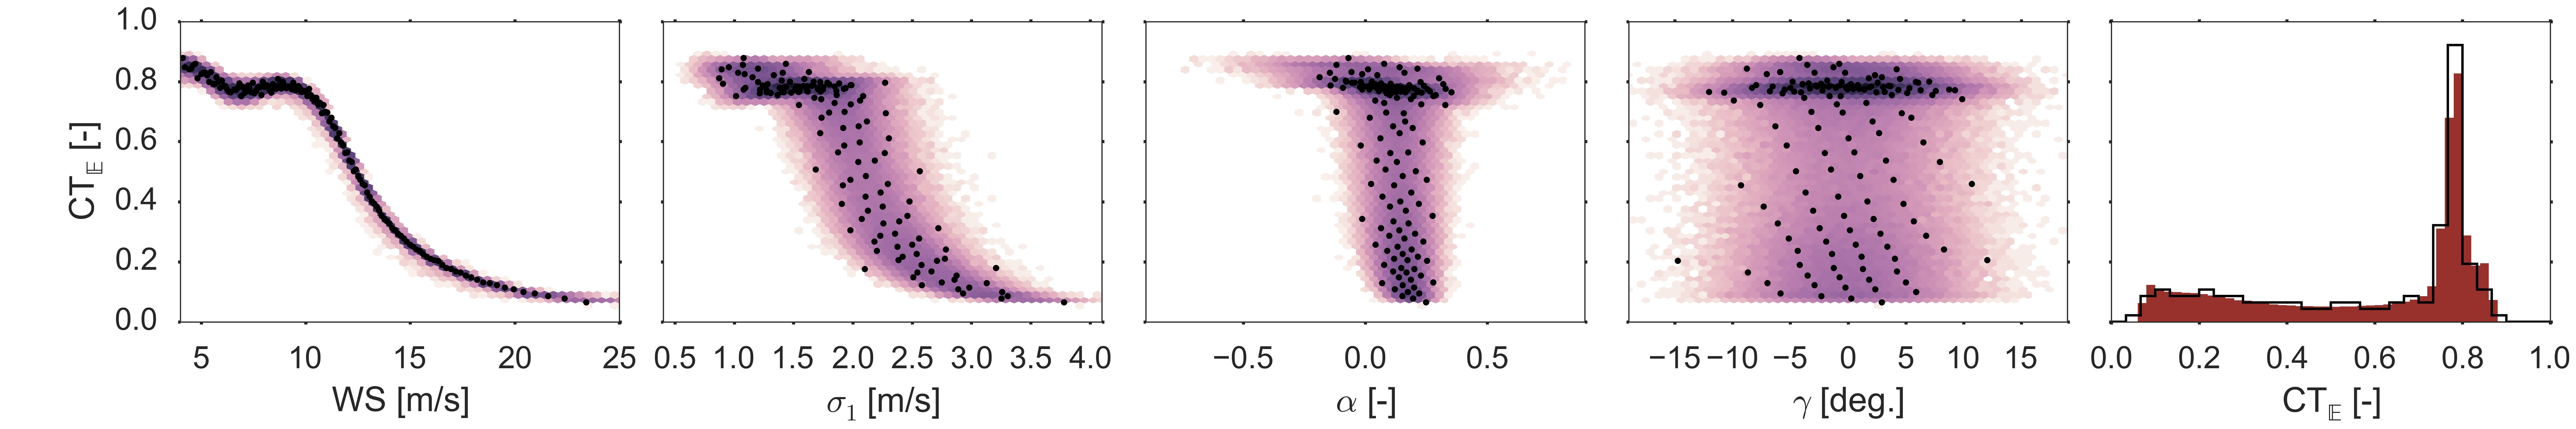
\includegraphics[width=\linewidth]{Figures/Surrgotes_20-fold/CT_E_MC_PCE_last_row.jpg} \\
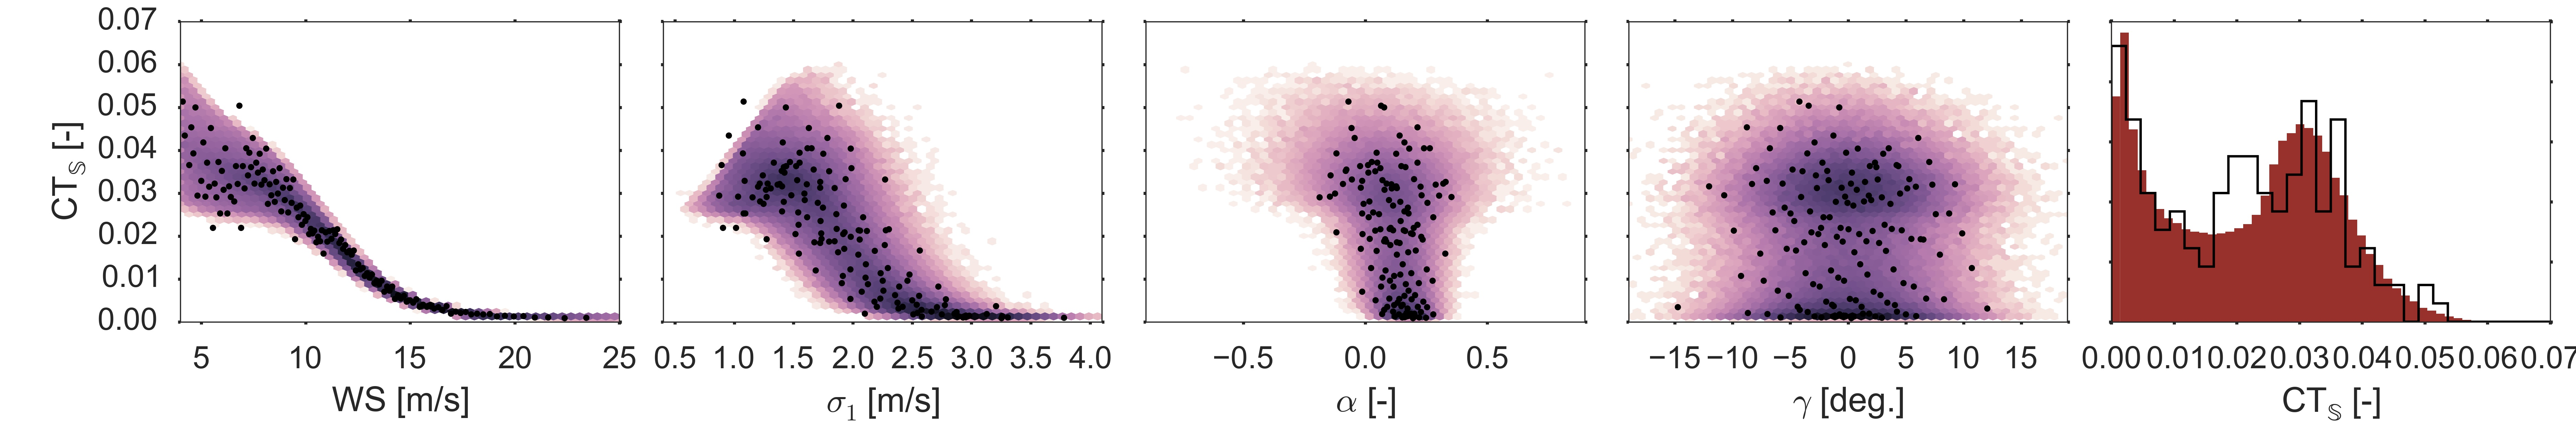
\includegraphics[width=\linewidth]{Figures/Surrgotes_20-fold/CT_S_MC_PCE_last_row.jpg}
\caption{Example surrogates for individual local statistical moments. (Black points) 140 training dataset. (Histogram colored hex-bins, lighter pink bins have lower probability) 80000 Monte-Carlo simulation on the surrogate.}
\label{fig_y_hat_E_V}
\end{centering}
\end{figure*}

The surrogates are robust enough to predict the frequency of occurrence of extreme values such as the outputs resulting from the input point with largest $\stdws$, see first and third row in figure \ref{fig_y_hat_E_V2}. This point seems to be outside the main trend in $\ws$ in figure \ref{fig_y_hat_E_V2} because it has a large $\stdws$ and $\shear$ given its $\ws$, see figure \ref{fig_PCE_train_x_full}.

\begin{figure*}[h!]
\begin{centering}
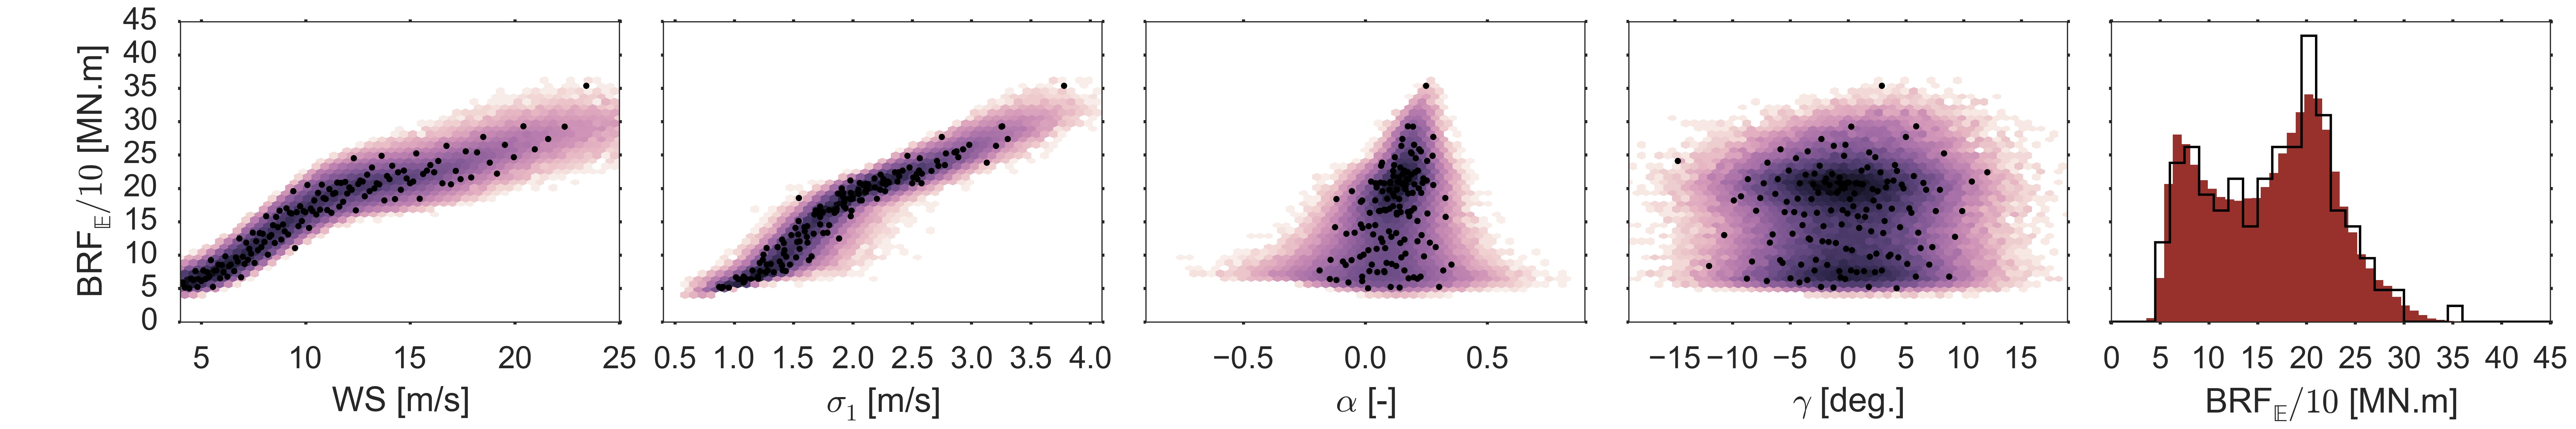
\includegraphics[width=\linewidth]{Figures/Surrgotes_20-fold/BRFBM_EFL_M12_E_MC_PCE_last_row.jpg} \\
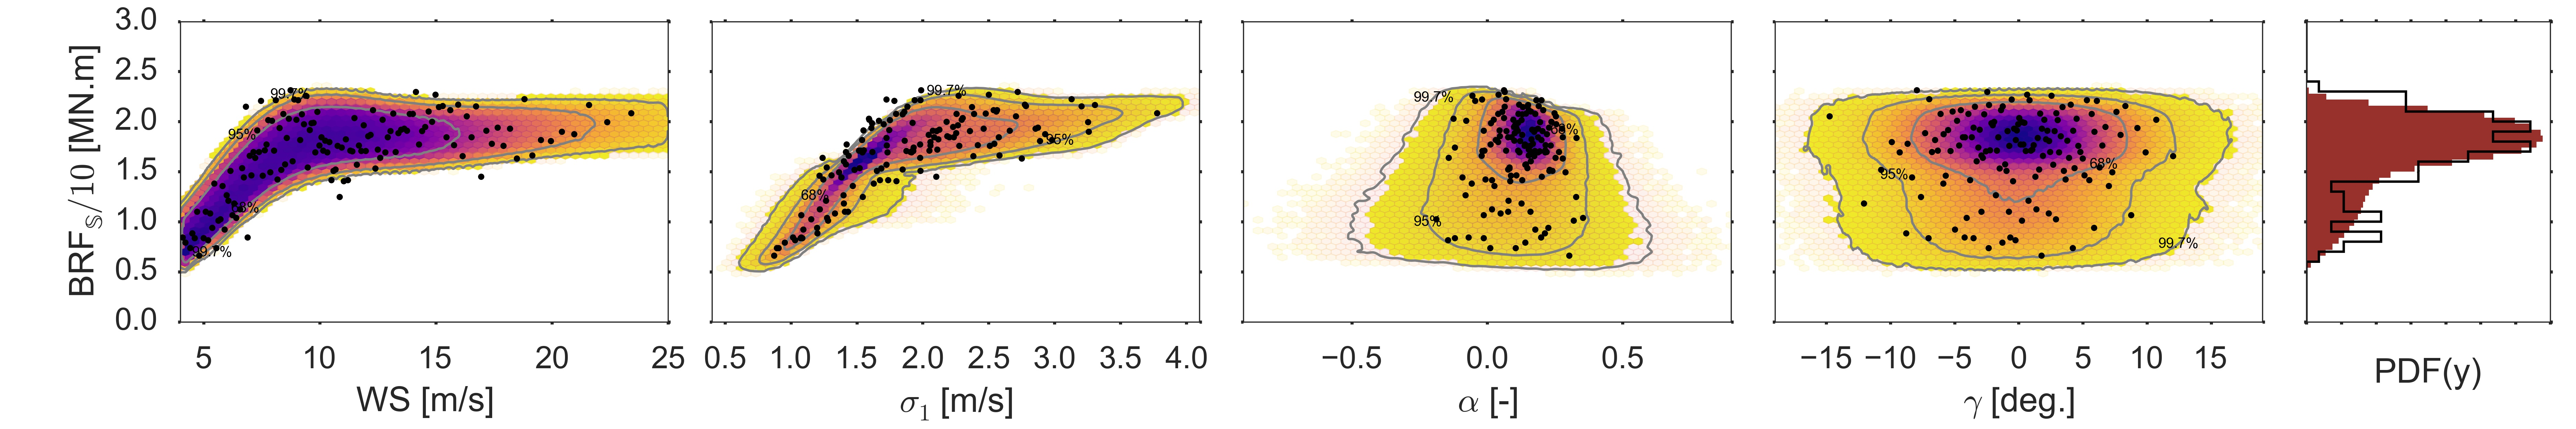
\includegraphics[width=\linewidth]{Figures/Surrgotes_20-fold/BRFBM_EFL_M12_S_MC_PCE_last_row.jpg} \\
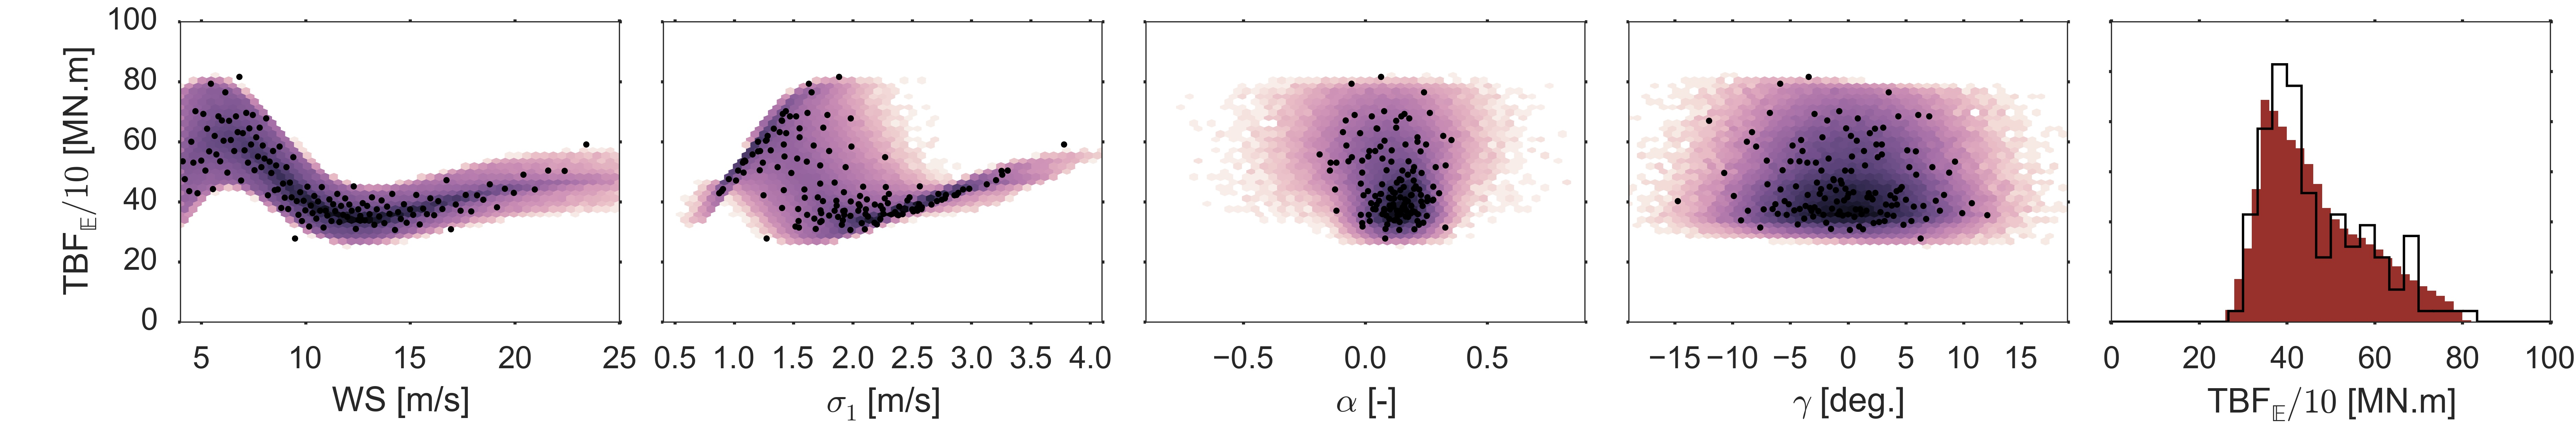
\includegraphics[width=\linewidth]{Figures/Surrgotes_20-fold/TBFBM_EFL_M4_E_MC_PCE_last_row.jpg} \\
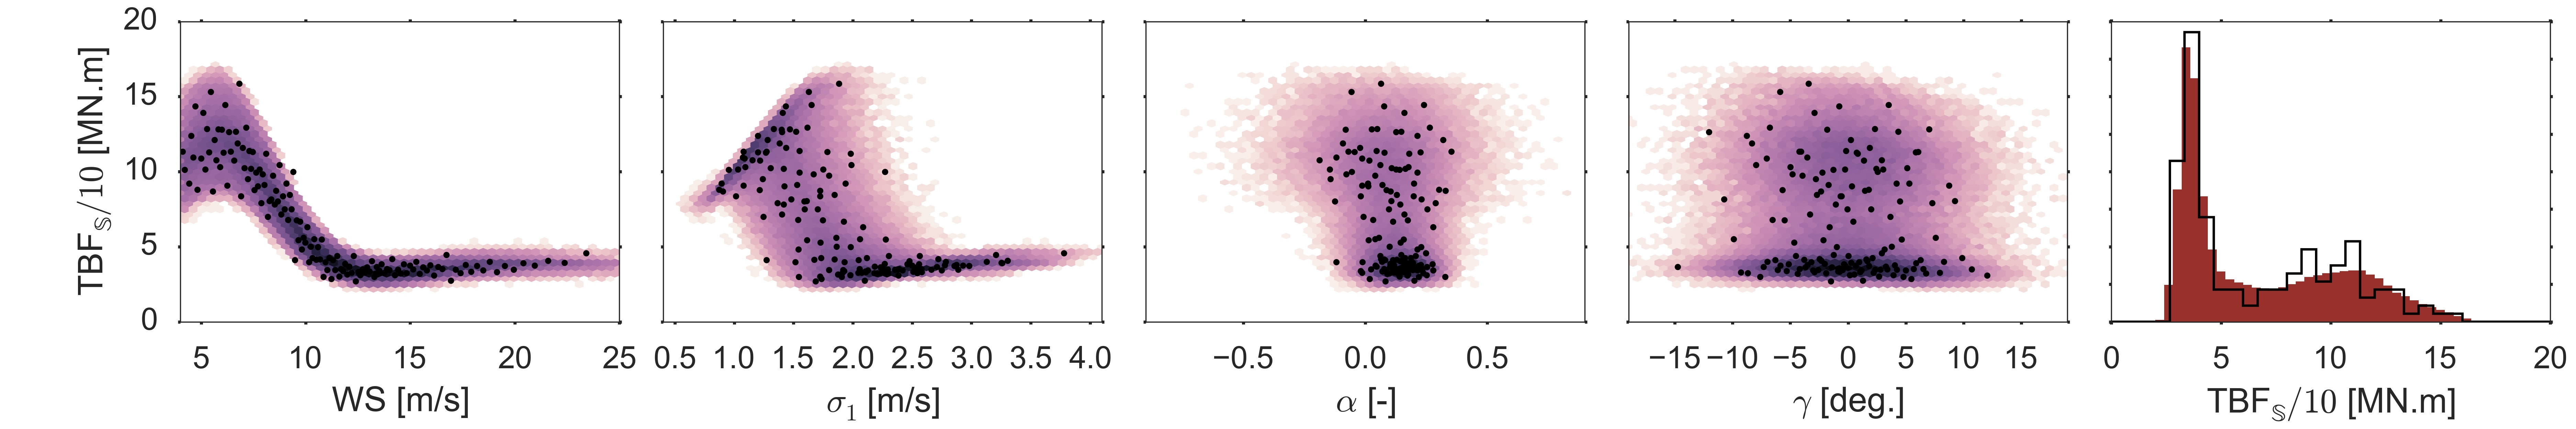
\includegraphics[width=\linewidth]{Figures/Surrgotes_20-fold/TBFBM_EFL_M4_S_MC_PCE_last_row.jpg}
\caption{Example surrogates for individual local statistical moments. (Black points) 140 training dataset. (Histogram colored hex-bins, lighter pink bins have lower probability) 80000 Monte-Carlo simulation on the surrogate.}
\label{fig_y_hat_E_V2}
\end{centering}
\end{figure*}


\subsection{Final surrogate predictions}
%%%

The final surrogates of the DTU 10 MW RWT obtained are presented in figure \ref{fig_final_surrogates}. The amount of local output variation due to the turbulent inflow realization varies between outputs and depends on the region of the input space. In the figure \ref{fig_final_surrogates}, each see-through black cross represents an individual realization of the turbulence. The effect of the turbulent inflow realization is more important for the fatigue loads. The final surrogate covers the space of model outputs and predicts the general details of the overall distributions of the outputs, see column 5 in figure \ref{fig_final_surrogates}.

\begin{figure}[p]
\begin{centering}
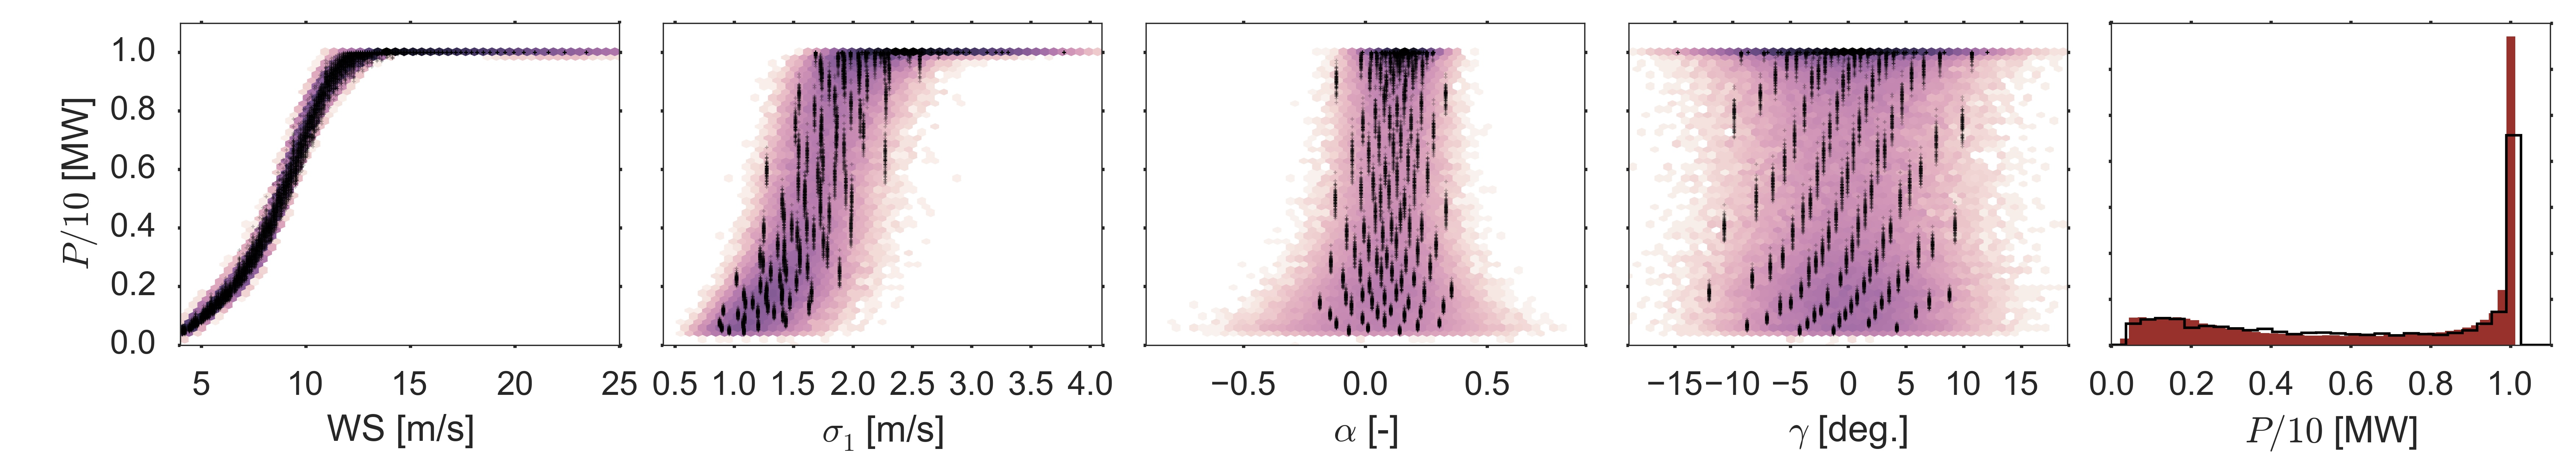
\includegraphics[width=\linewidth]{Figures/Full_surrogate_red_file/P_PCE_MC_surrogate_last_row.jpg} \\
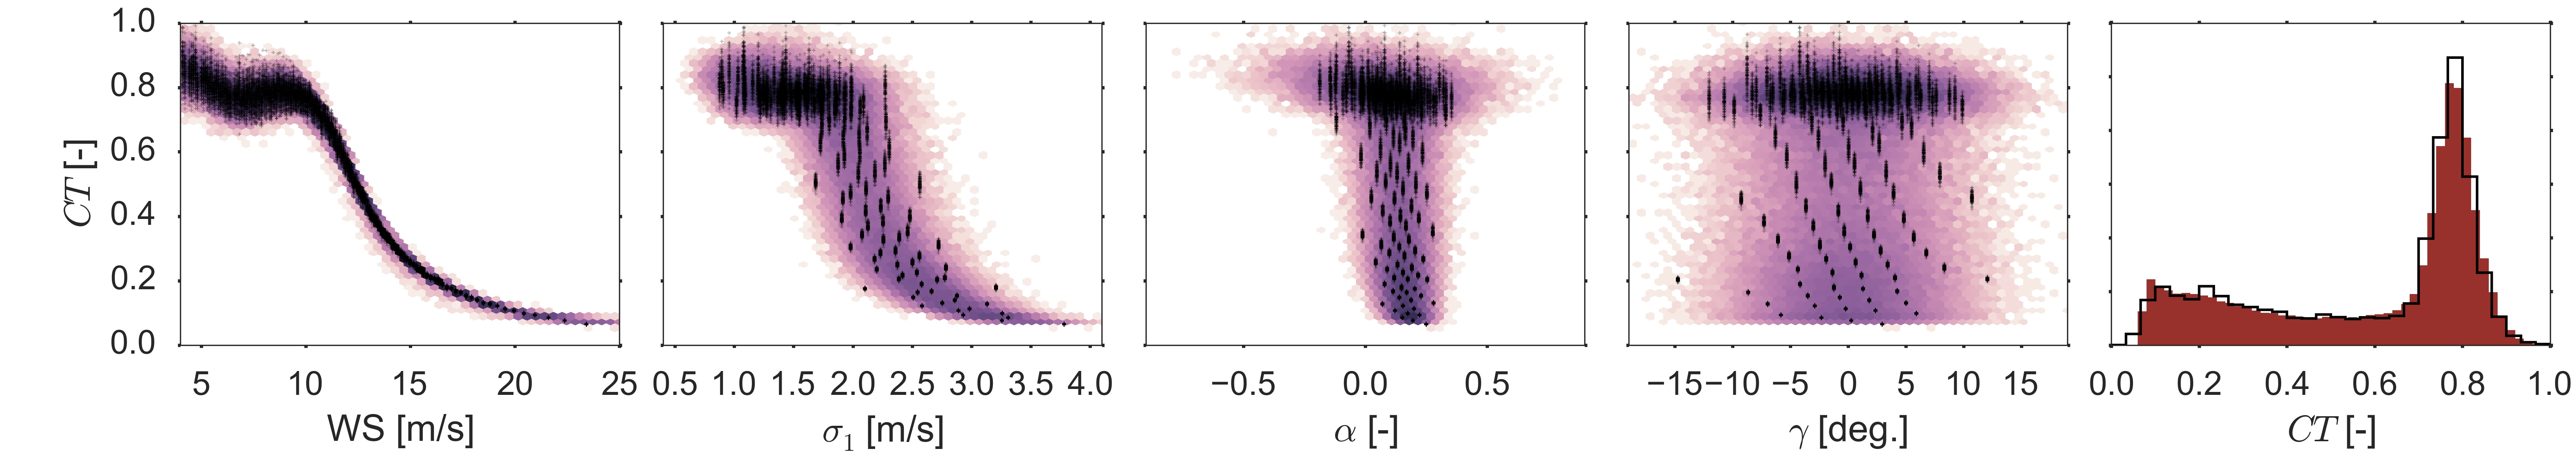
\includegraphics[width=\linewidth]{Figures/Full_surrogate_red_file/CT_PCE_MC_surrogate_last_row.jpg} \\
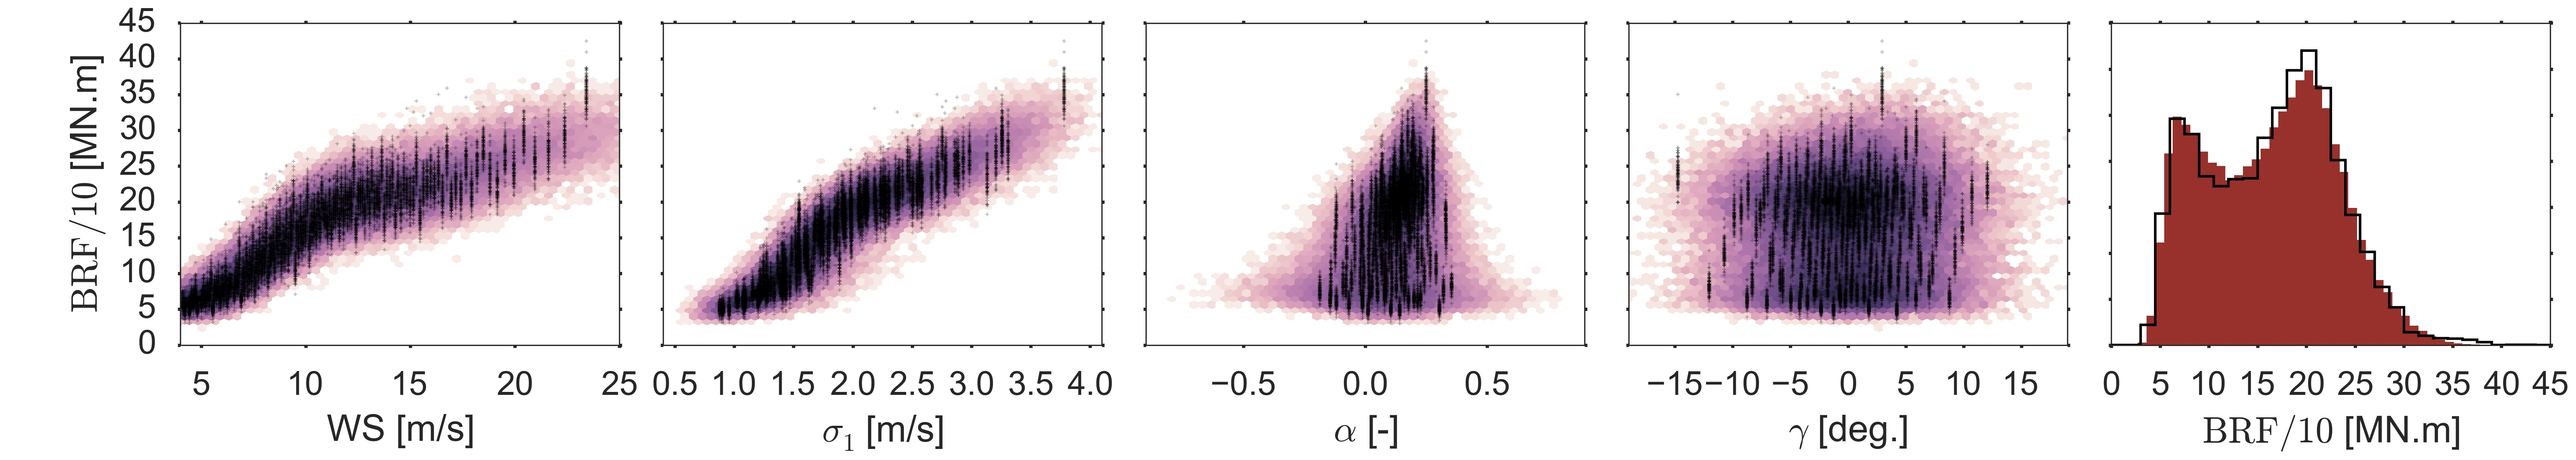
\includegraphics[width=\linewidth]{Figures/Full_surrogate_red_file/BRFBM_EFL_M12_PCE_MC_surrogate_last_row.jpg} \\
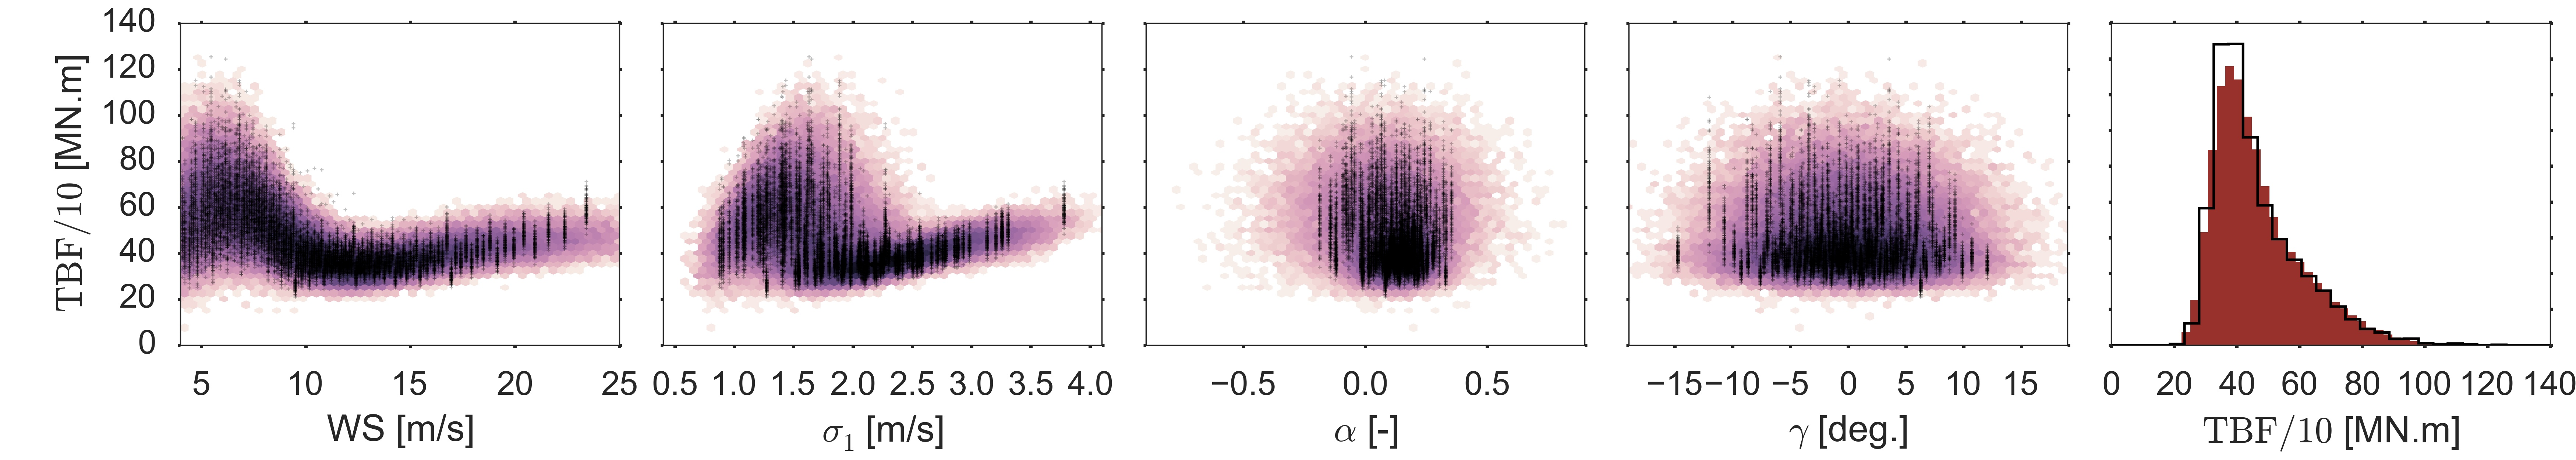
\includegraphics[width=\linewidth]{Figures/Full_surrogate_red_file/TBFBM_EFL_M4_PCE_MC_surrogate_last_row.jpg} \\
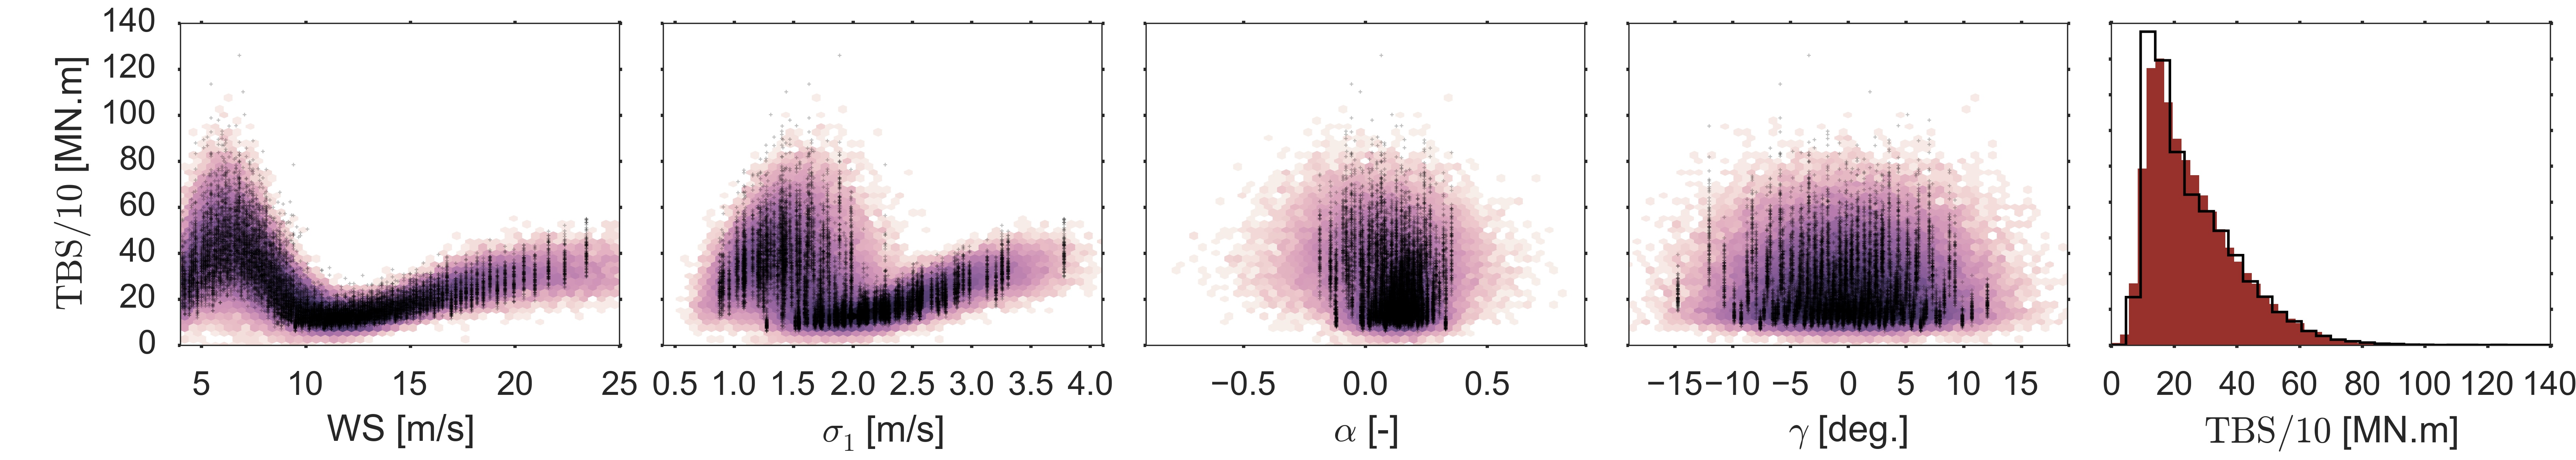
\includegraphics[width=\linewidth]{Figures/Full_surrogate_red_file/TBSBM_EFL_M4_PCE_MC_surrogate_last_row.jpg} \\
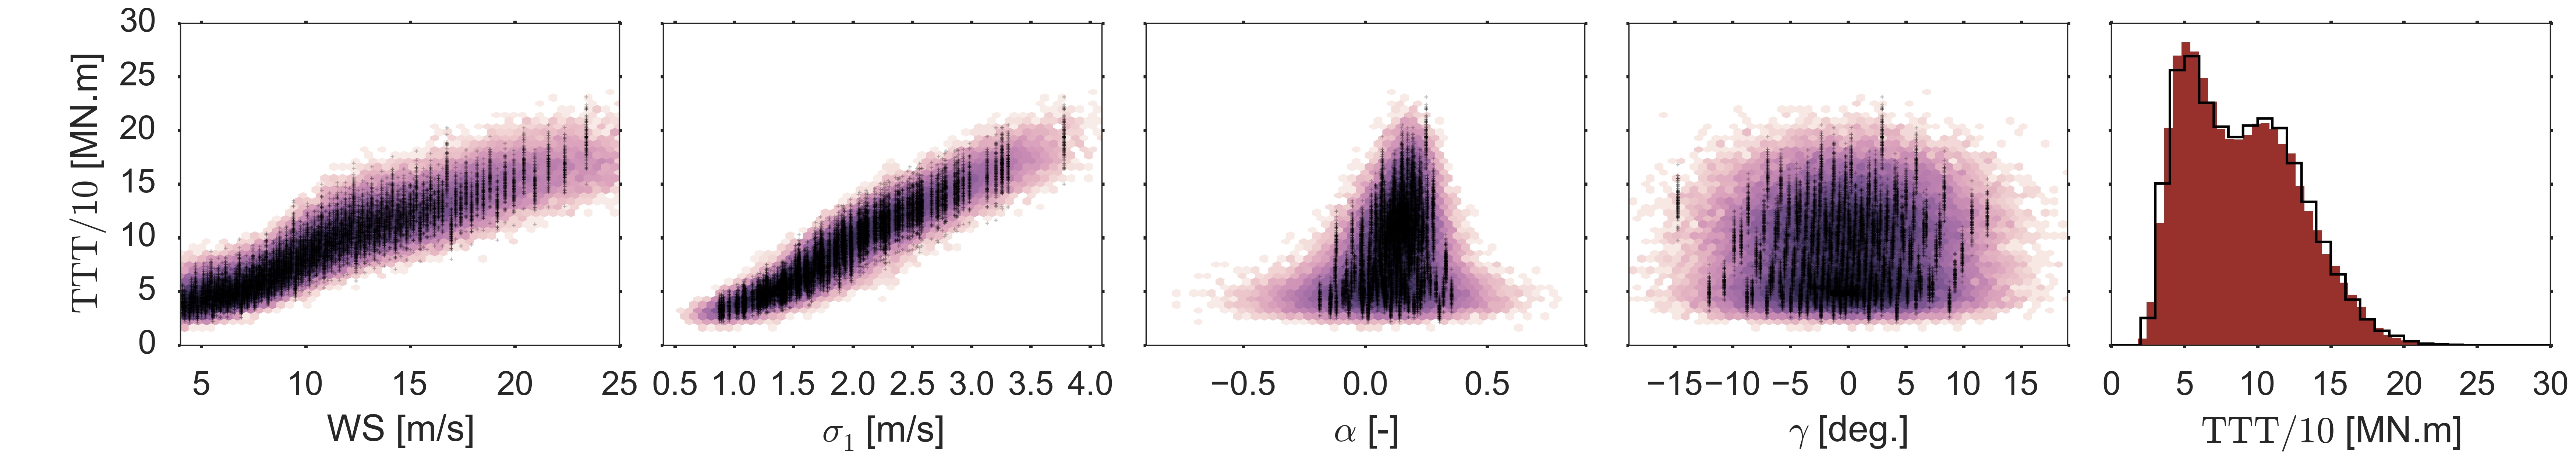
\includegraphics[width=\linewidth]{Figures/Full_surrogate_red_file/TTTBM_EFL_M4_PCE_MC_surrogate_last_row.jpg} \\
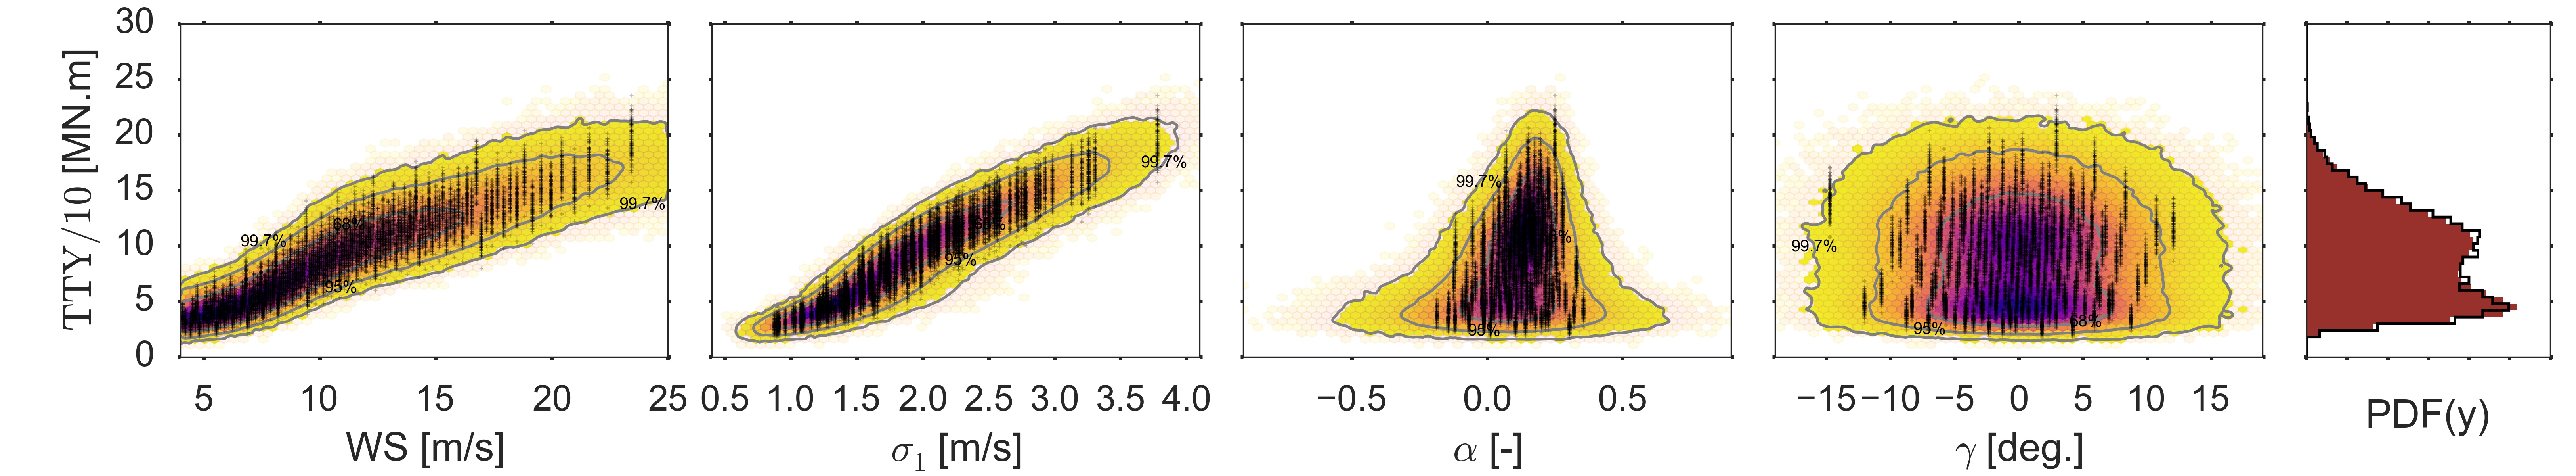
\includegraphics[width=\linewidth]{Figures/Full_surrogate_red_file/TTYBM_EFL_M4_PCE_MC_surrogate_last_row.jpg}
\caption{(Black points) Training dataset in the outputs: 140 Hammersley sequence sample x 100 turbulent inflow realizations. (Histogram colored hex-bins, lighter pink bins have lower probability) 80000 Monte-Carlo simulation of the surrogate.}
\label{fig_final_surrogates}
\end{centering}
\end{figure}

\subsection{Sensitivity analysis}

The global sensitivity analysis (SA) for the outputs are presented in table \ref{tab_sens}. The total effect Sobol indexes are computed using the approximation presented by Saltelli et al \cite{saltelli2010variance}. The total effect Sobol indexes represents the non-linear influence of the input variable in the total variance of the output. Most of the outputs have a large total Sobol index for the wind speed. $\ws$ is clearly the main variable to explain the power and loads in a wind turbine. The SA shows that the local expected value of power and thrust coefficient can be explained almost fully with $\ws$.

The variance introduced by the turbulent inflow realization is an important component for all the outputs, it has a higher influence than $\stdws$ for most outputs. This counterintuitive result is due to the large amount of correlation between $\ws$ and $\stdws$, therefore a large fraction of the variance due to $\stdws$ is already explained by $\ws$. The shear and yaw have reduced effects over most output variables. The yaw miss alignment has reduced total effect because its assumed distribution is centered around zero. The shear exponent becomes important only for capturing the fatigue at the tower top tilt and yaw bending moments (TTT, TTY); while the yaw misalignment becomes important for modeling the fatigue at the tower bottom fore-aft moment (TBF).

\begin{table}[!h]
\begin{centering}
\resizebox{0.8\linewidth}{!}{
\begin{tabular}{cccccc}
\hline
Output &      $\ws$ &  $\stdws$ &   $\shear$ &     $\yaw$ &  Turb\_realization \\
\hline
\\[-1em]
P             & $1$ &   $3\times 10^{-4}$ &  $3\times 10^{-4}$ & $1\times 10^{-4}$ &      $4\times 10^{-3}$ \\
 & 1st & 3rd-4th & 3rd-4th & 5th & 2nd \\
\hline
\\[-1em]
CT            & $1$ &   $1\times 10^{-3}$ &  $1\times 10^{-3}$ & $7\times 10^{-4}$ &      $1\times 10^{-2}$ \\
 & 1st & 3rd-4th & 3rd-4th & 5th & 2nd \\
\hline
\\[-1em]
BRF & $9\times 10^{-1}$ &   $5\times 10^{-2}$ &  $1\times 10^{-2}$ & $3\times 10^{-3}$ &      $7\times 10^{-2}$ \\
 & 1st & 3rd & 4th & 5th & 2nd \\
\hline
\\[-1em]
TBF  & $6\times 10^{-1}$ &   $2\times 10^{-1}$ &  $3\times 10^{-4}$ & $1\times 10^{-3}$ &      $3\times 10^{-1}$ \\
 & 1st & 3rd & 5th & 4th & 2nd \\
\hline
\\[-1em]
TBS  & $7\times 10^{-1}$ &   $7\times 10^{-2}$ &  $2\times 10^{-3}$ & $2\times 10^{-4}$ &      $3\times 10^{-1}$ \\
 & 1st & 3rd & 4th-5th & 4th-5th & 2nd \\
\hline
\\[-1em]
TTT  & $9\times 10^{-1}$ &   $7\times 10^{-2}$ &  $3\times 10^{-4}$ & $6\times 10^{-4}$ &      $8\times 10^{-2}$ \\
 & 1st & 2nd-3rd & 4th & 5th & 2nd-3rd \\
\hline
\\[-1em]
TTY  & $9\times 10^{-1}$ &   $7\times 10^{-2}$ &  $2\times 10^{-4}$ & $1\times 10^{-3}$ &      $7\times 10^{-2}$ \\
 & 1st & 3rd-4th & 3rd-4th & 5th & 2nd
\end{tabular}}
\caption{Total sensitivity indexes (Total influence Sobol indexes).}
\label{tab_sens}
\end{centering}
\end{table}



\subsection{Convergence}
\label{subsec_Convergence}

A leave-one-out cross-validation (LOO) is done to estimate the distribution of the prediction error of each surrogate as a function of the number of independent turbulent seeds. A LOO is equivalent to a k-fold validation in which the number of folds is the number of data points. This means that the surrogate is trained using 139 input points with a different number of turbulent inflow realizations per input point. Then, the local statistical moments of the output predicted by the surrogates at the missing point are compared against the statistics computed using the full 100 realizations. In this article, the prediction errors are normalized with respect to the maximum scale of the output variable, which means that the errors represent the fraction of the total scale that should be considered as an extra uncertainty due to the inadequacy of the surrogate. The prediction error for the local mean surrogate is defined as:

\eq{\eyE = \frac{y_{\expect}(\vx_{LO}) - \hat{y}_{\expect}(\vx_{LO})}{\max(y)}}{}

\noindent while the prediction error for the local standard deviation surrogate is defined as:

\eq{\eyS = \frac{y_{\std}(\vx_{LO}) - \hat{y}_{\std}(\vx_{LO})}{\max(y)}}{}

%\eq{CV_E = \left| 1- \frac{\hat{y}_{\expect}(\vx_{LO})}{y_{\expect}(\vx_{LO})} \right| \quad \quad CV_S = \left| 1- \frac{\hat{y}^2_{\std}(\vx_{LO})}{y^2_{\std}(\vx_{LO})} \right|^{1/2}}{eq_CV_EV}

%\eq{CV_A = \frac{\int_{-\infty}^{\infty} |CDF(y_{PCE}|\vx=\vx_{LO})-CDF_{emp}(y|\vx=\vx_{LO})|\, dy}{\max(y)}}{eq_CV_A}

The convergence of the prediction error of the statistical moments is shown in figure \ref{fig_convergence}. It can be seen that all the prediction errors tend to be distributed around zero and their standard deviations converge as the number of turbulent inflow realizations per input are increased. The errors converge to the distribution of the errors to the current surrogate. New input points need to be added to the training data set in order to further narrow the converged distribution of surrogate errors. In this figure the outliers are the extreme cases of selecting seeds with similar outputs, therefore, they are those cases that have large errors in the statistical moments. Finally, the converged distribution can be used to estimate the uncertainty in the final prediction of the output as:

\eq{\hat{y}(\vx) \sim \text{Normal} (\hat{y}_{\expect}(\vx)+\eyE \, max(y), \quad \hat{y}_{\std}(\vx)+\eyS \, max(y))}{eq_output_distrib_U}

\noindent where the errors of the surrogates can be sampled from the distribution predicted using LOO cross validation, see figure \ref{fig_convergence}:

\eq{\eyE \sim \text{Normal}(\expect(\eyE),\std(\eyE)) \quad \eyS \sim \text{Normal}(\expect(\eyS),\std(\eyS))}{}

\begin{figure}[h!]
\begin{centering}
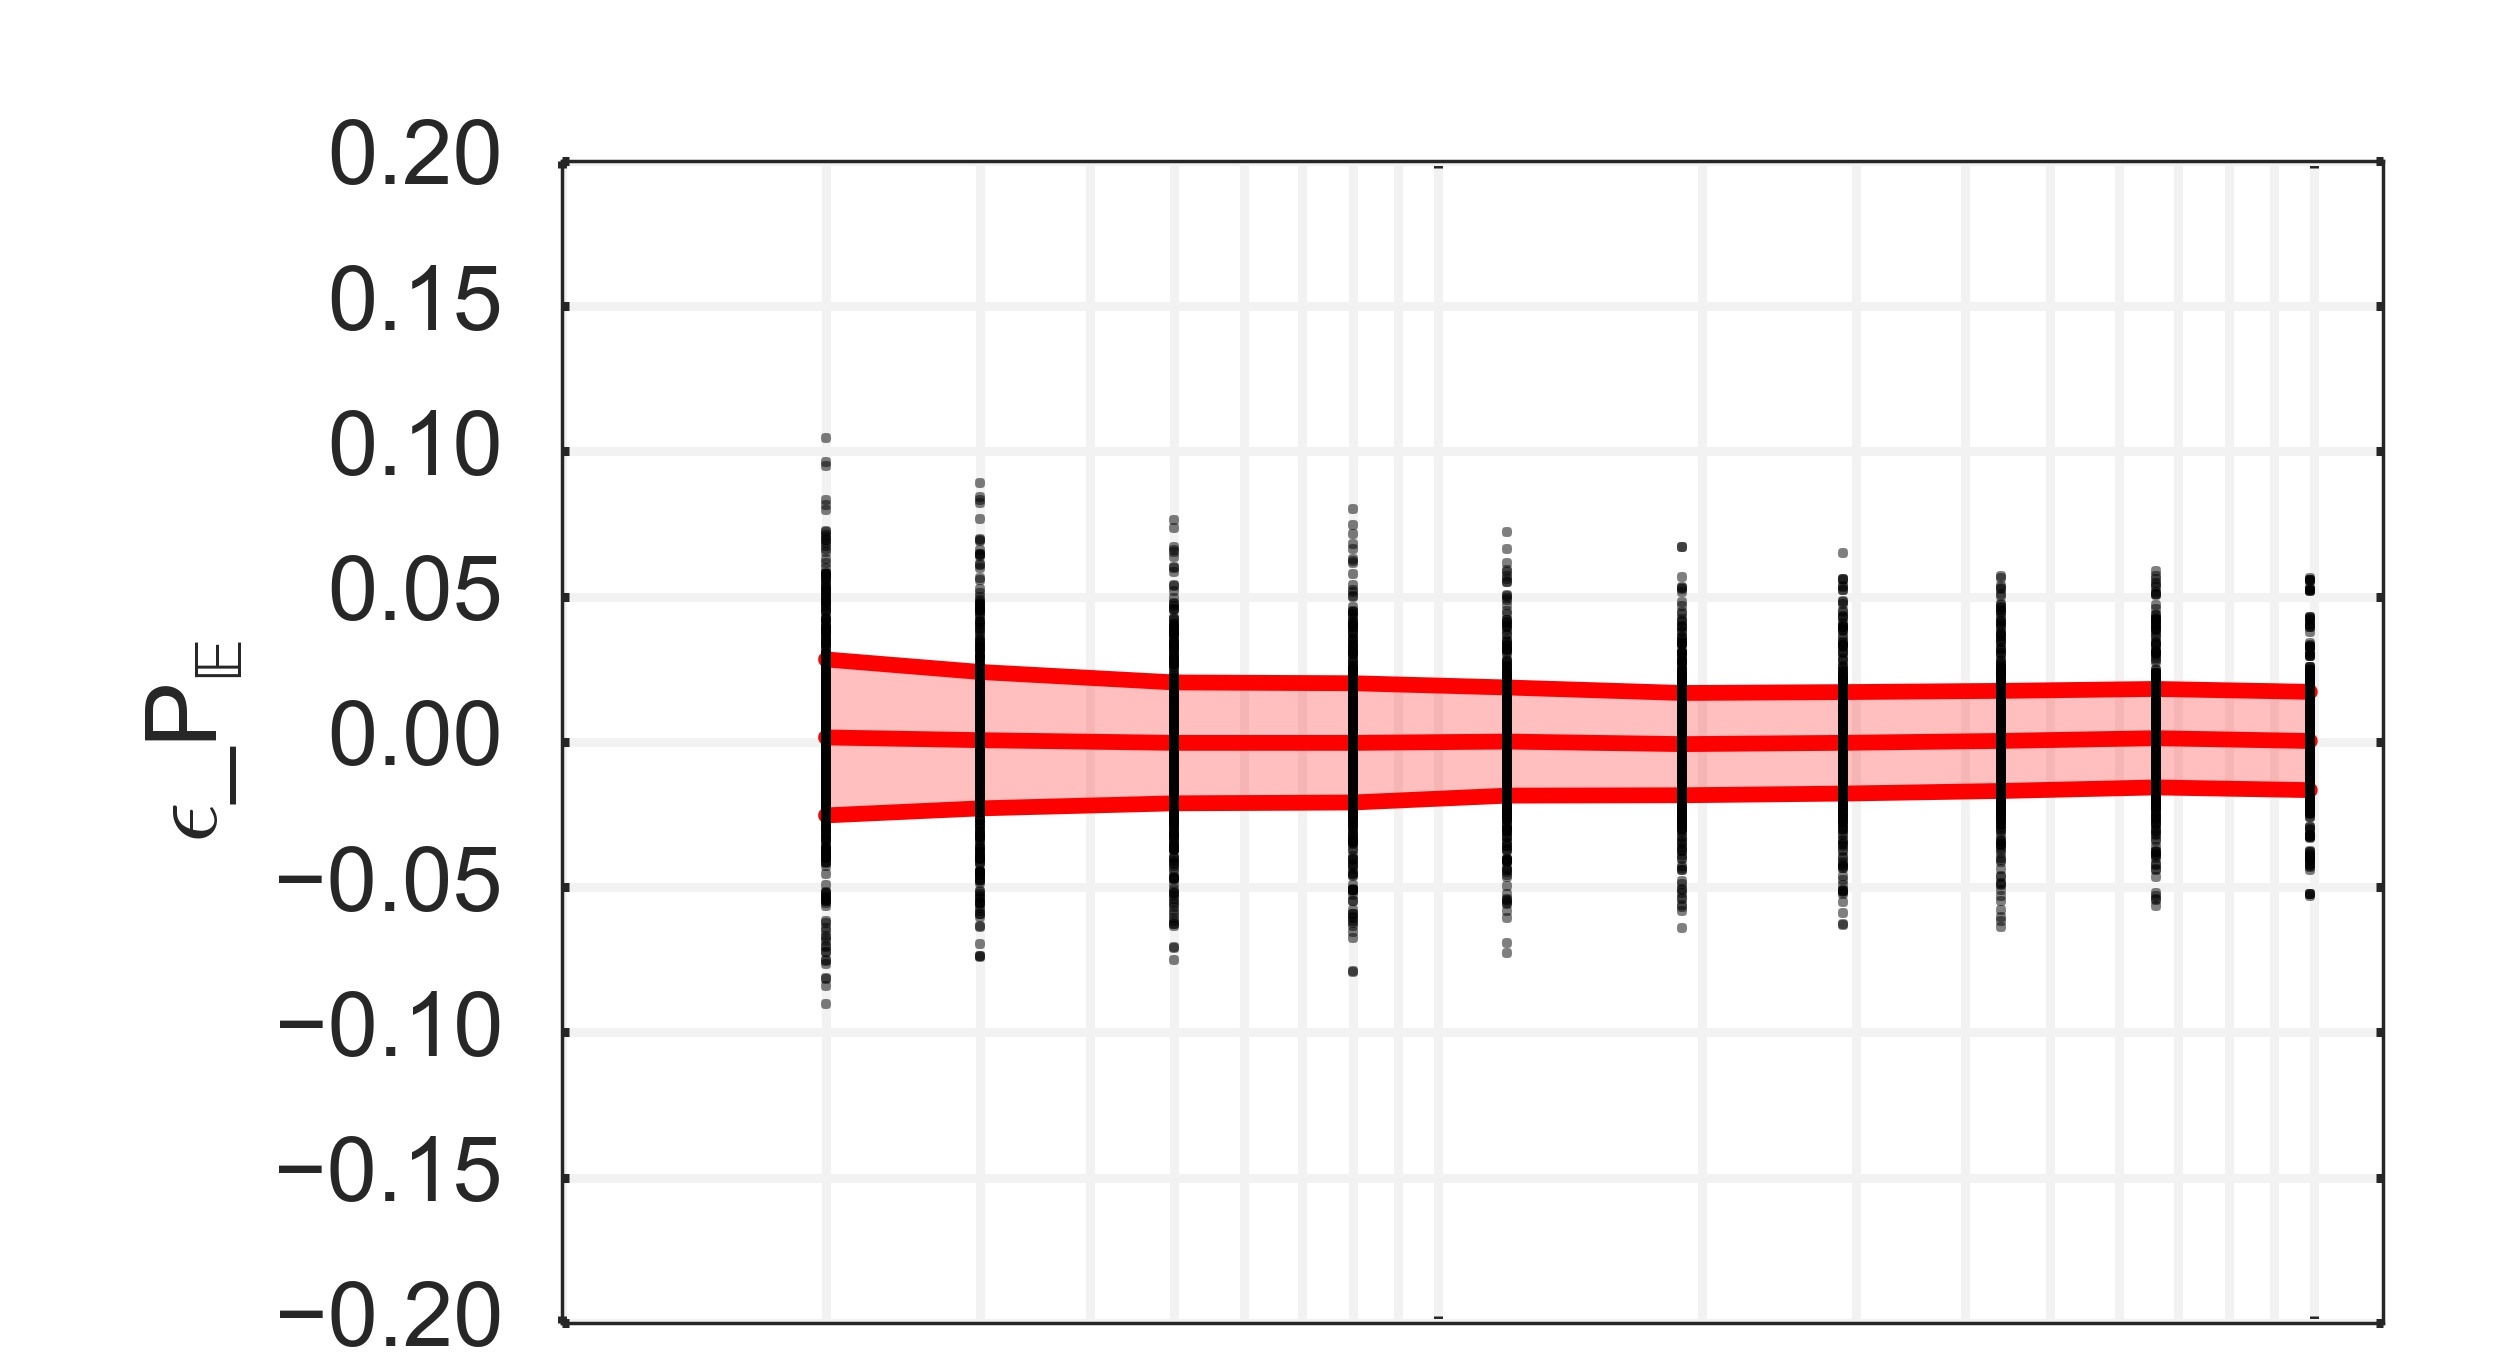
\includegraphics[width=0.32\columnwidth]{Figures/Convergence/CV_E_P.jpg}
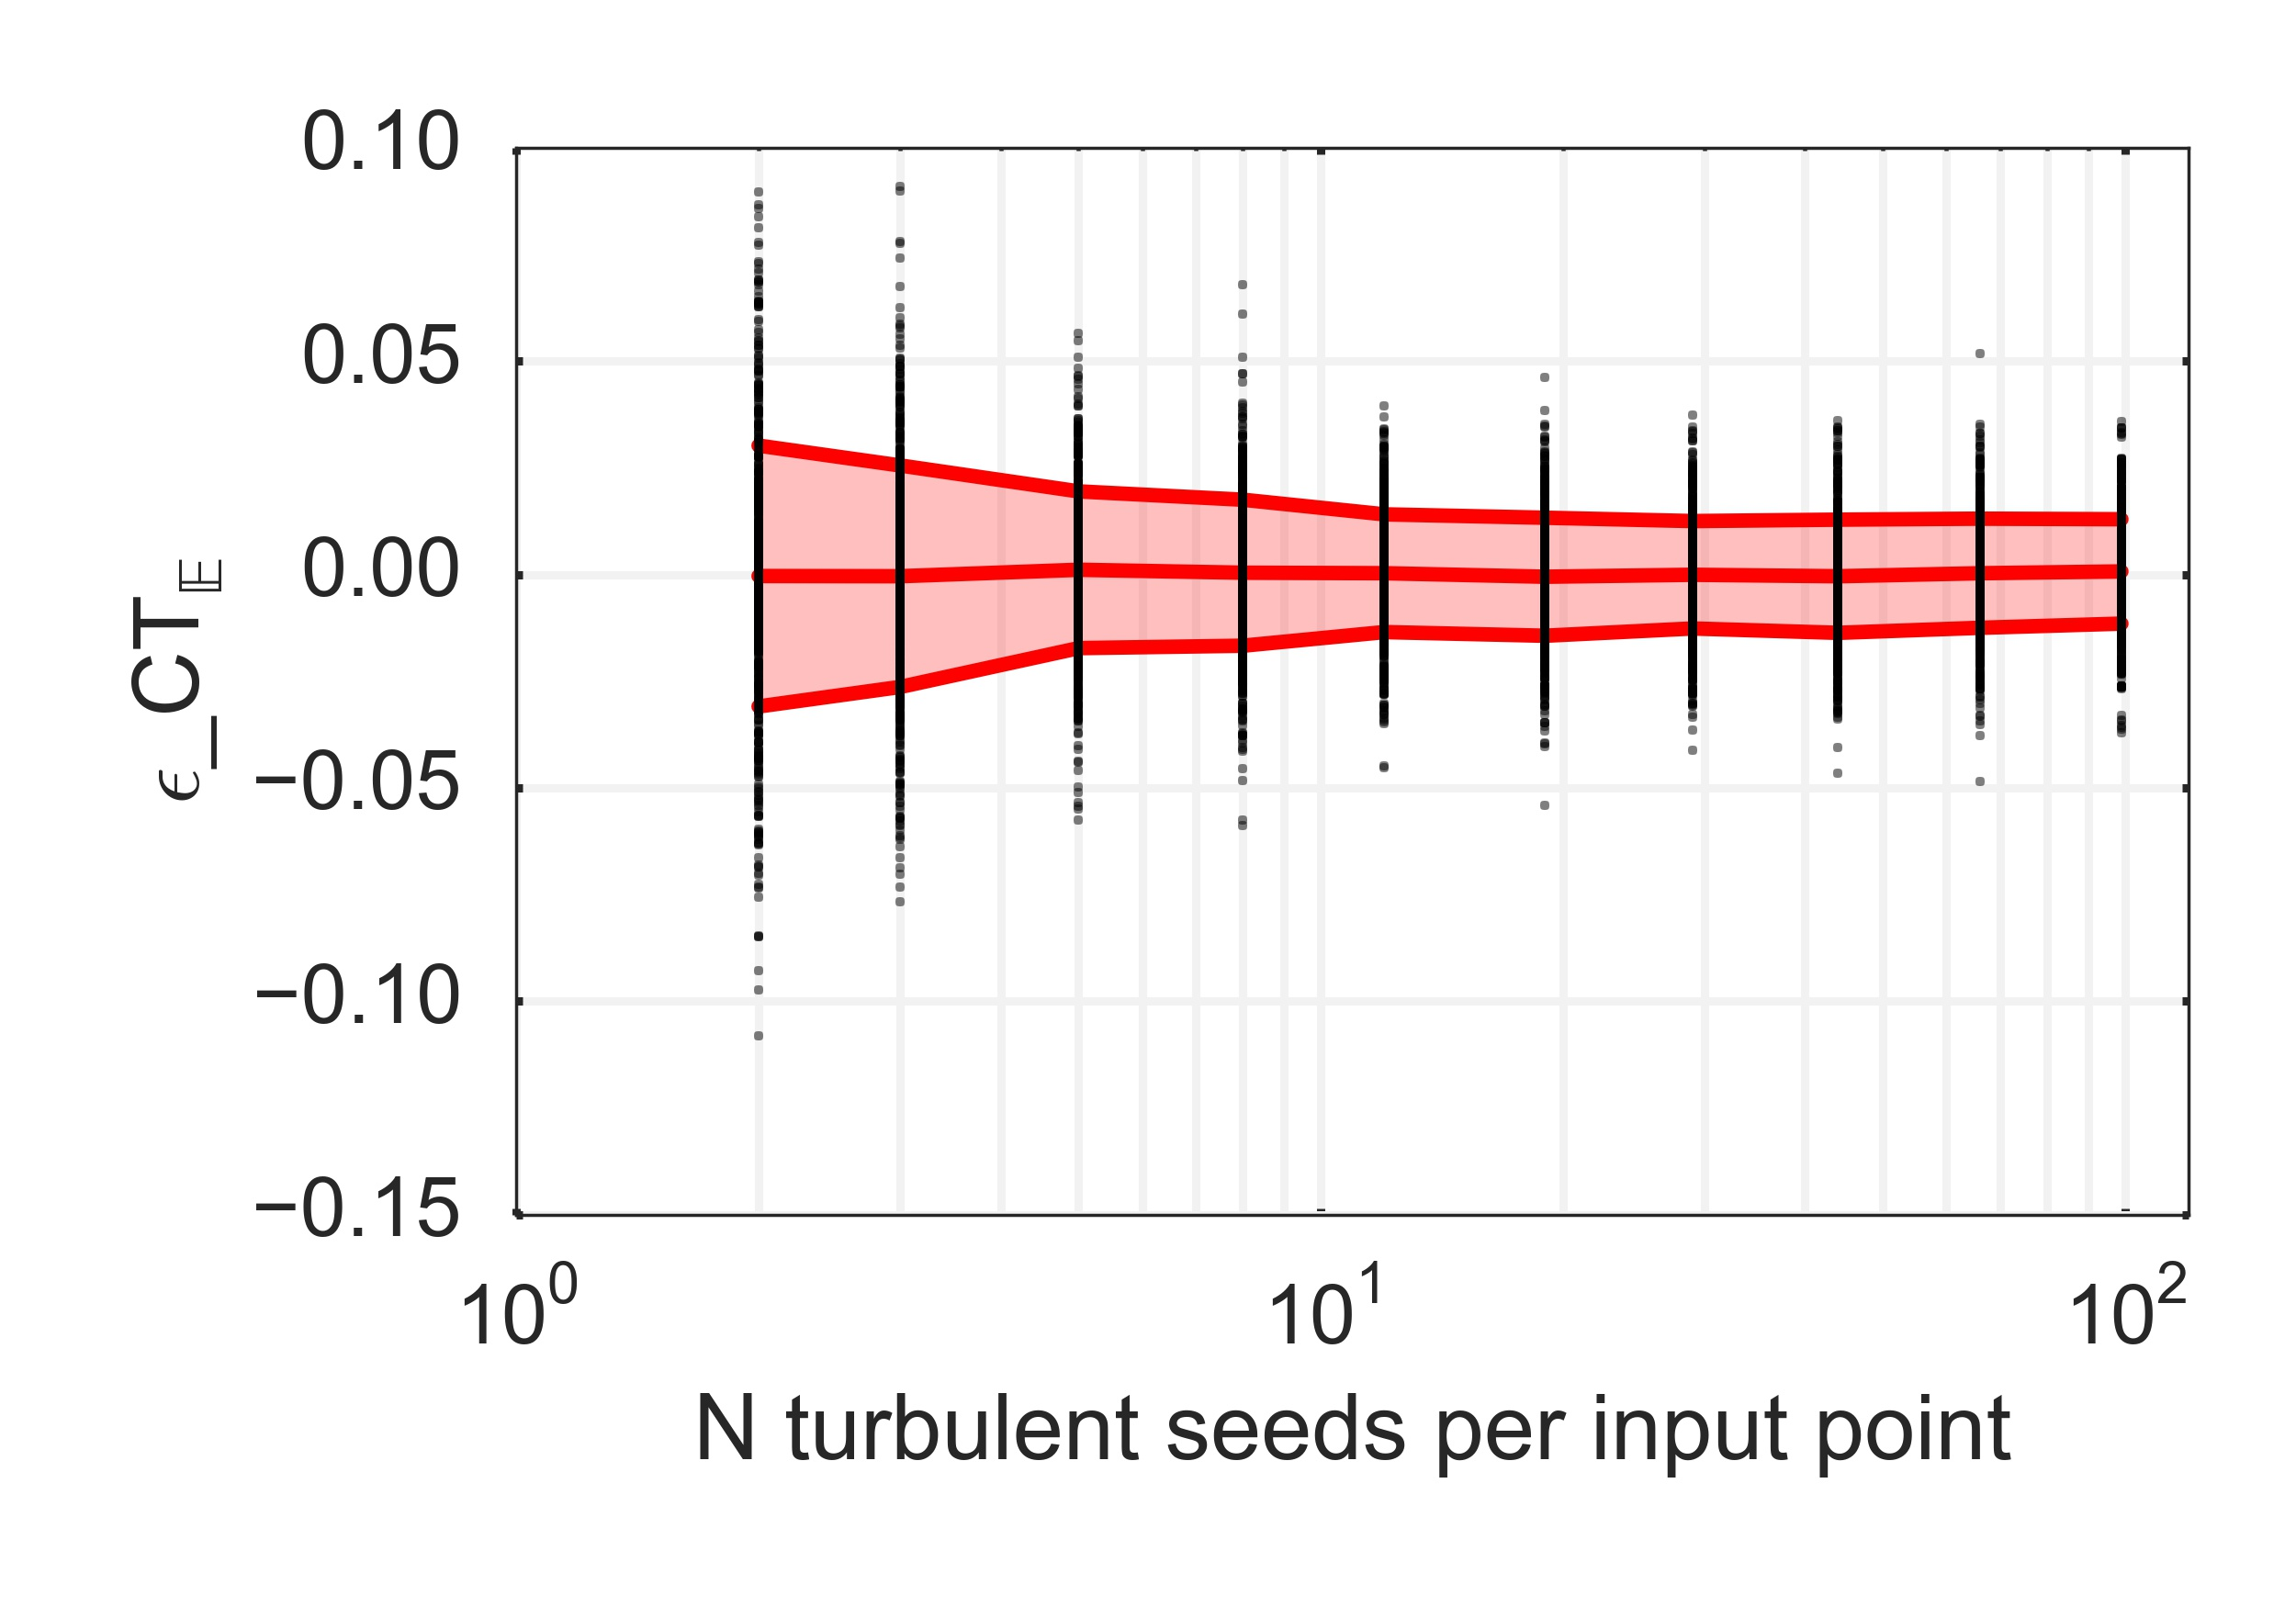
\includegraphics[width=0.32\columnwidth]{Figures/Convergence/CV_E_CT.jpg}
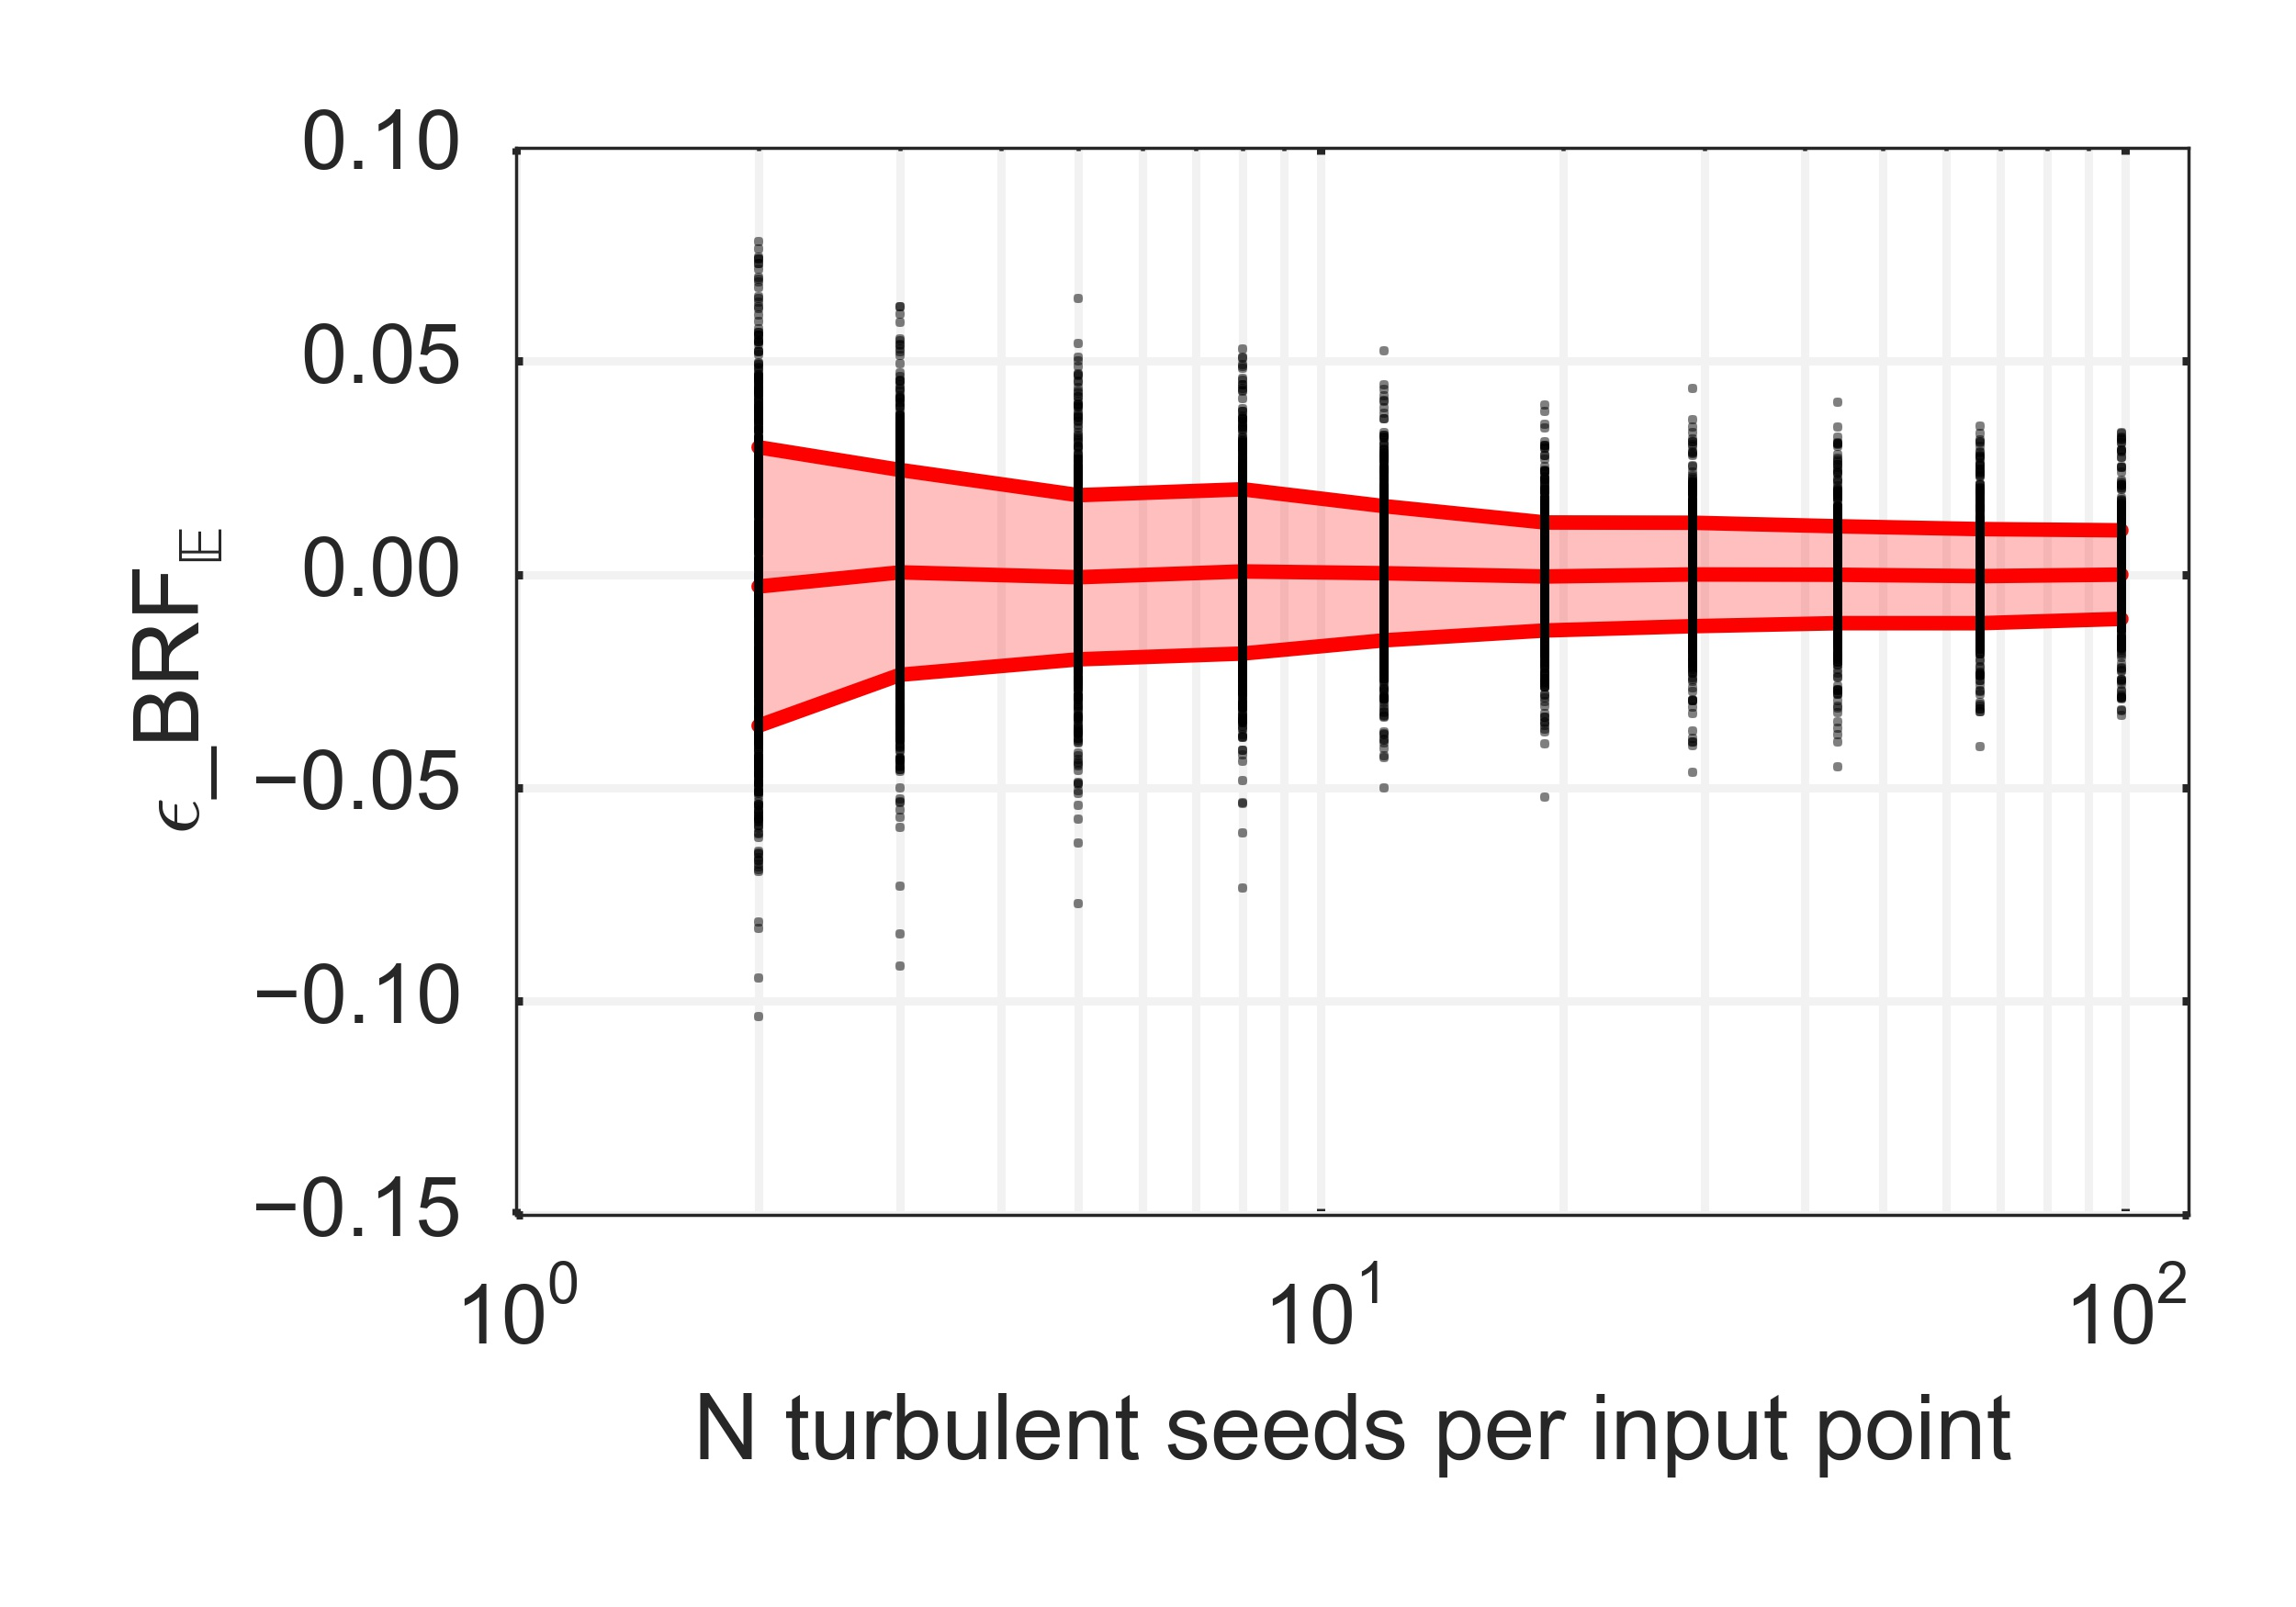
\includegraphics[width=0.32\columnwidth]{Figures/Convergence/CV_E_BRFBM_EFL_M12.jpg} \\
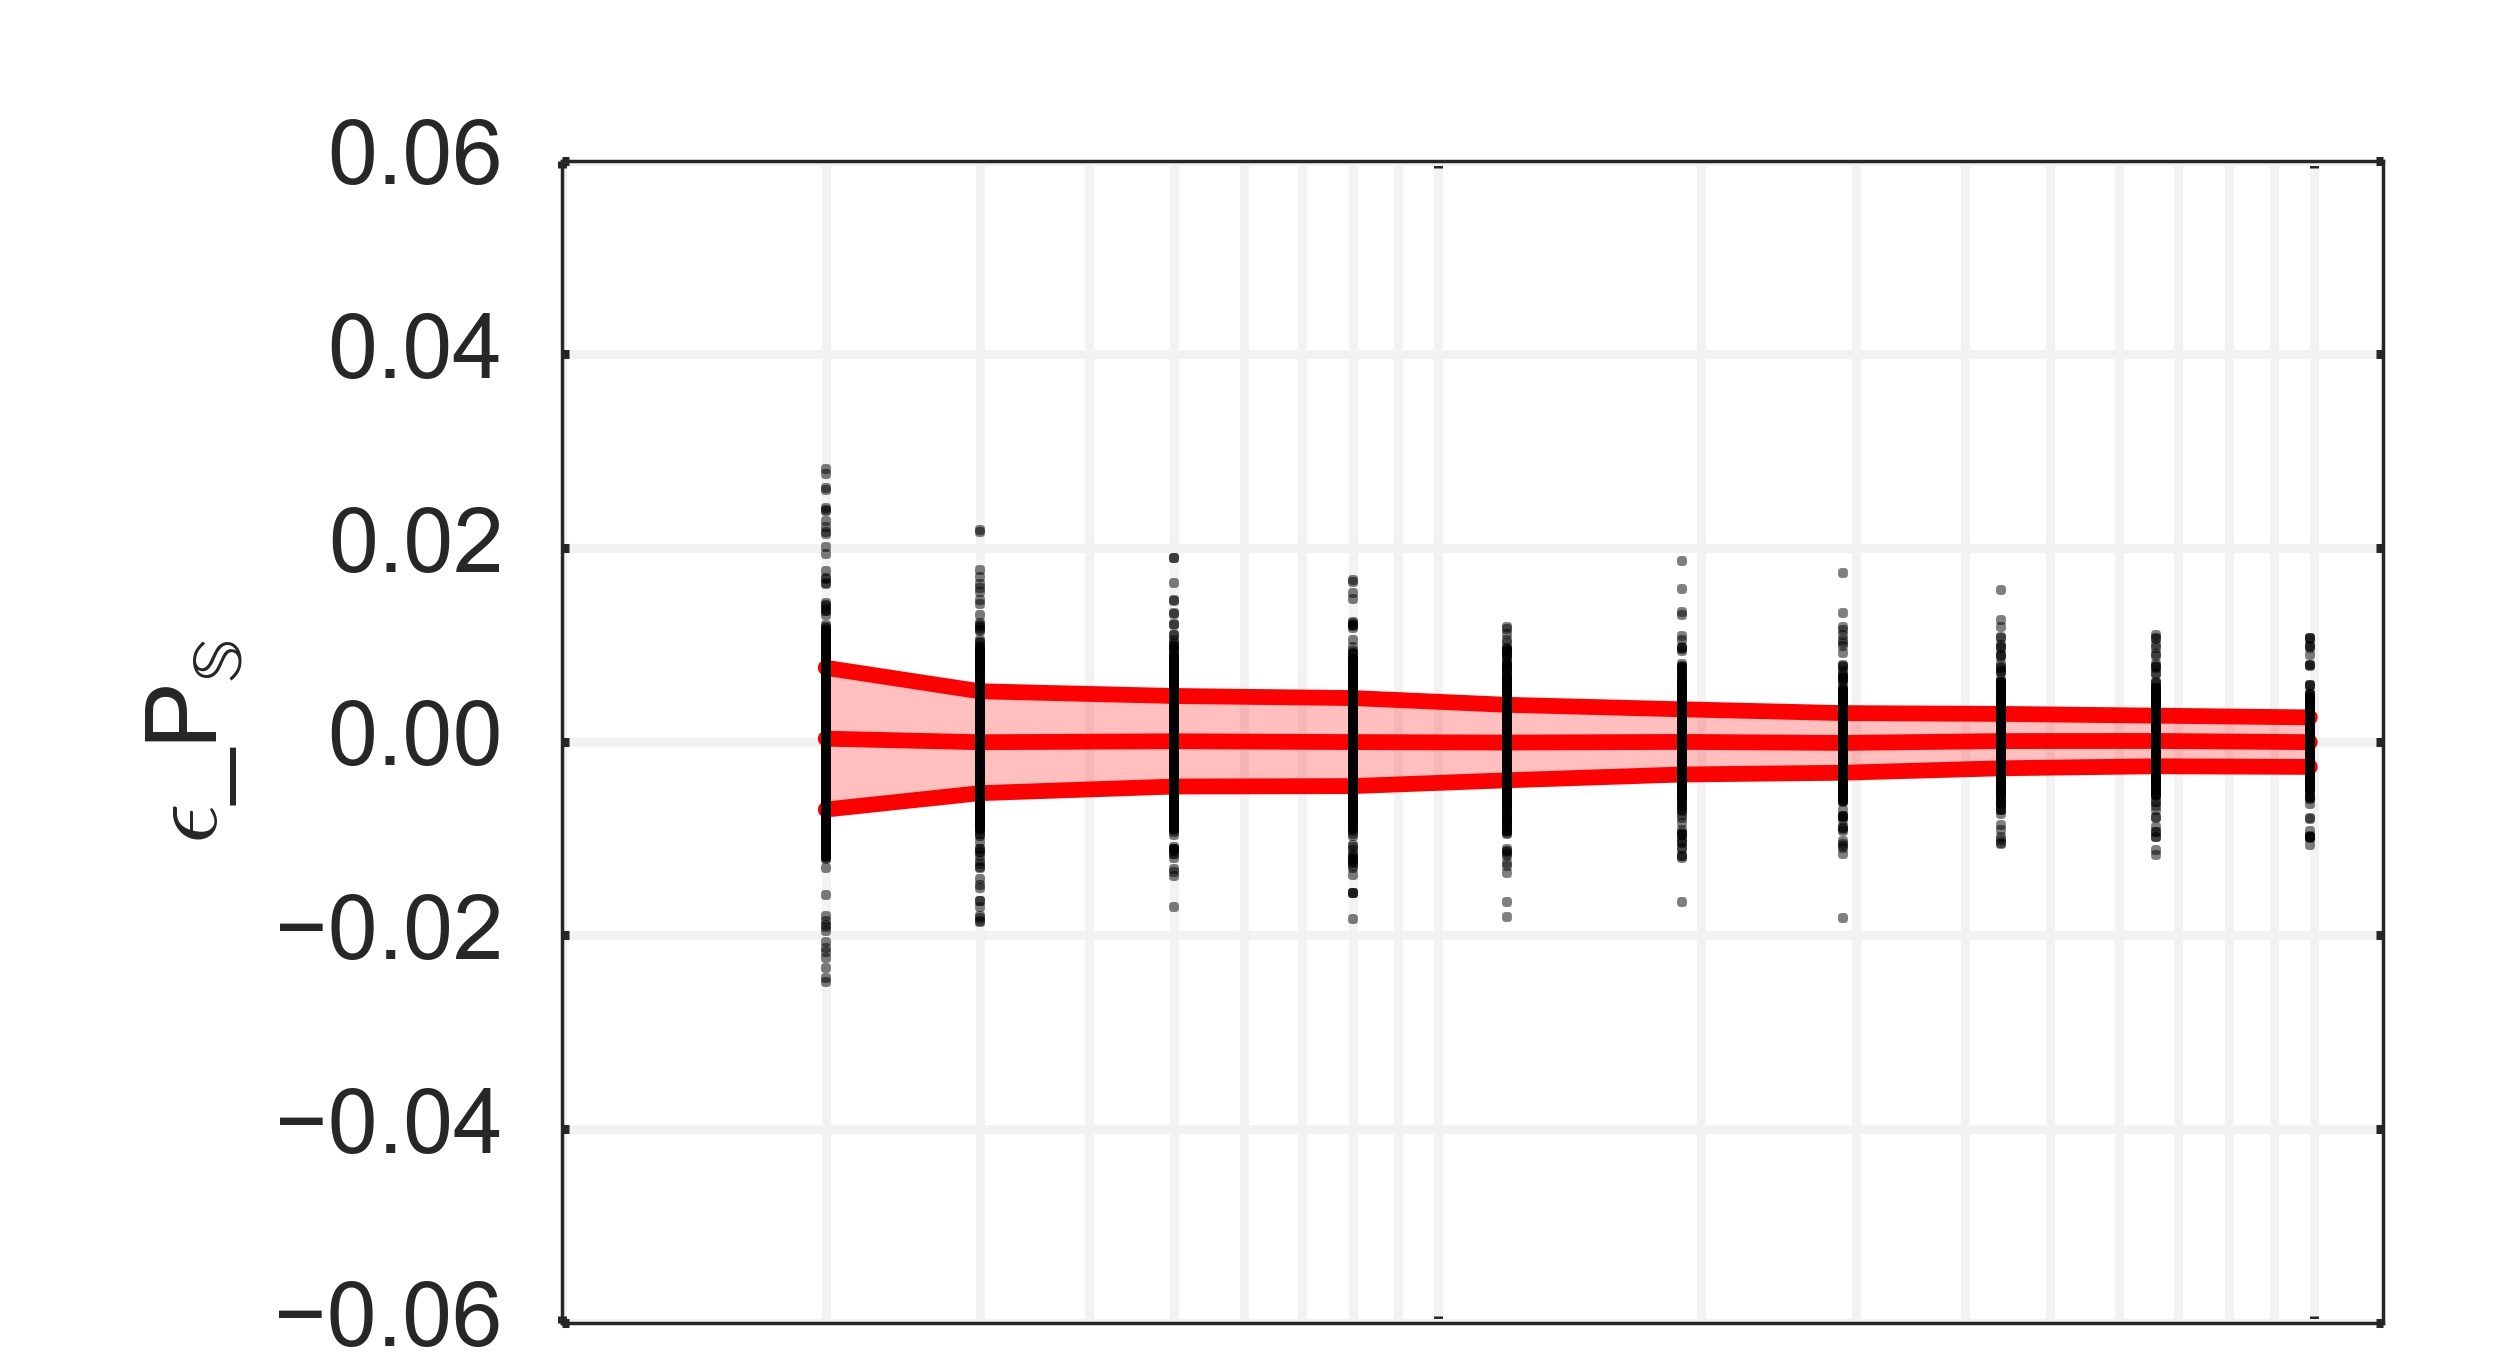
\includegraphics[width=0.32\columnwidth]{Figures/Convergence/CV_V_P.jpg}
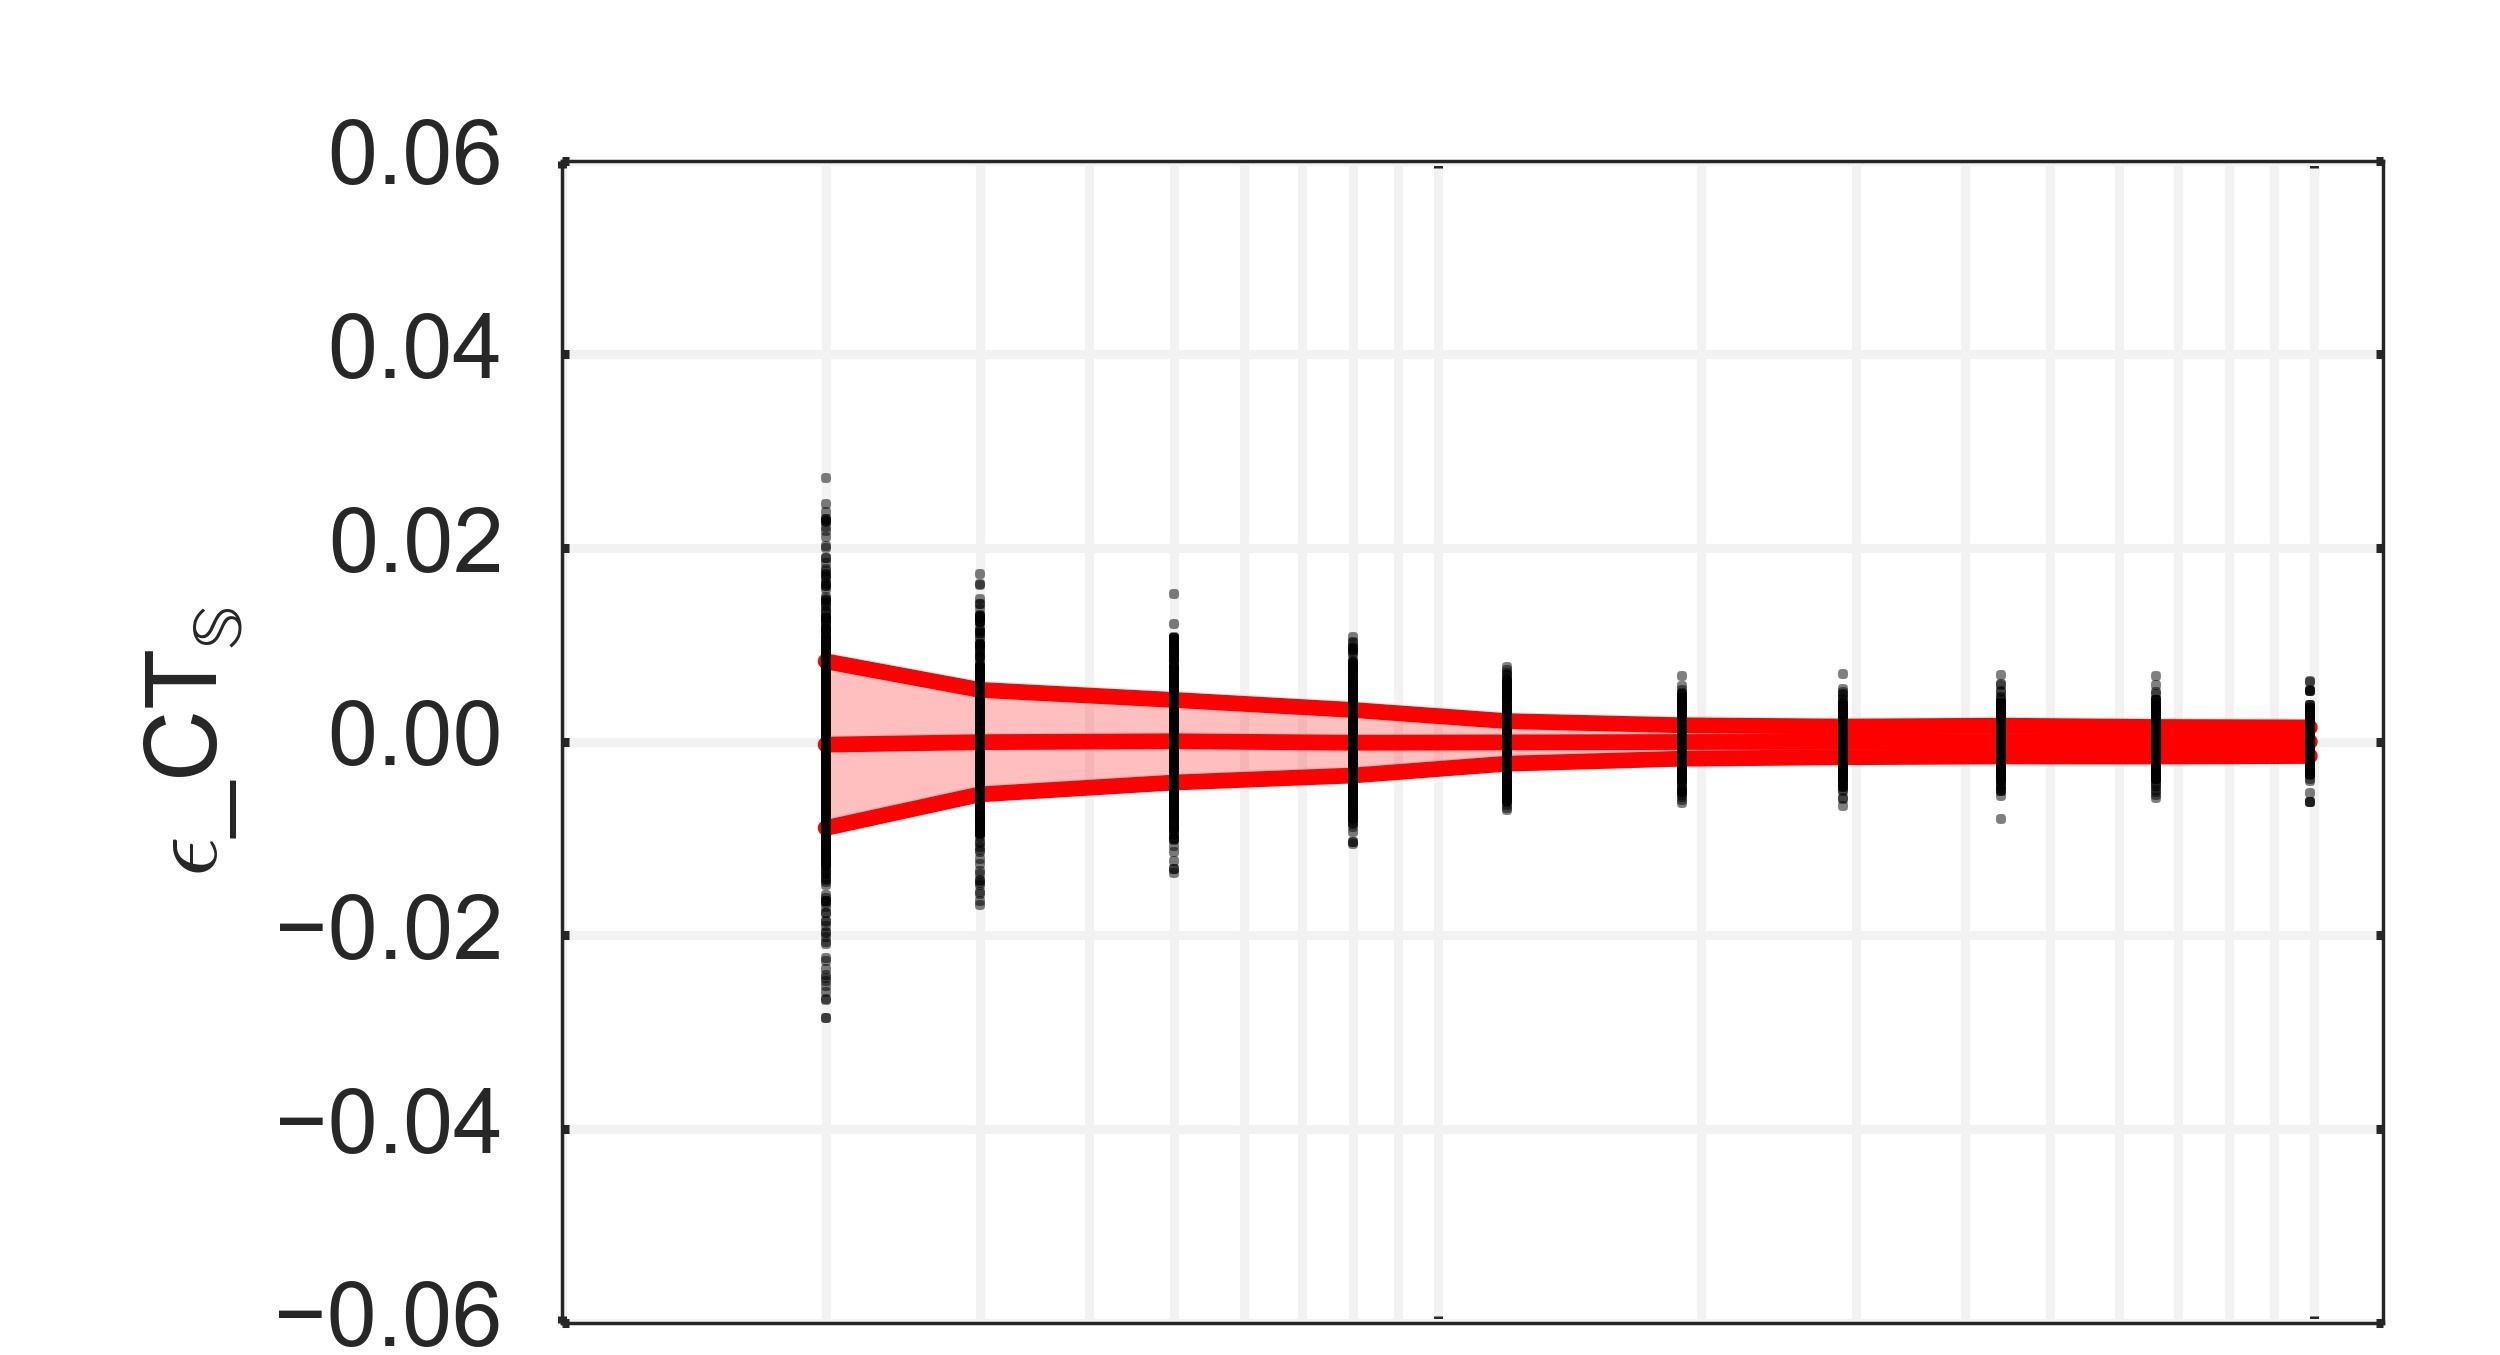
\includegraphics[width=0.32\columnwidth]{Figures/Convergence/CV_V_CT.jpg}
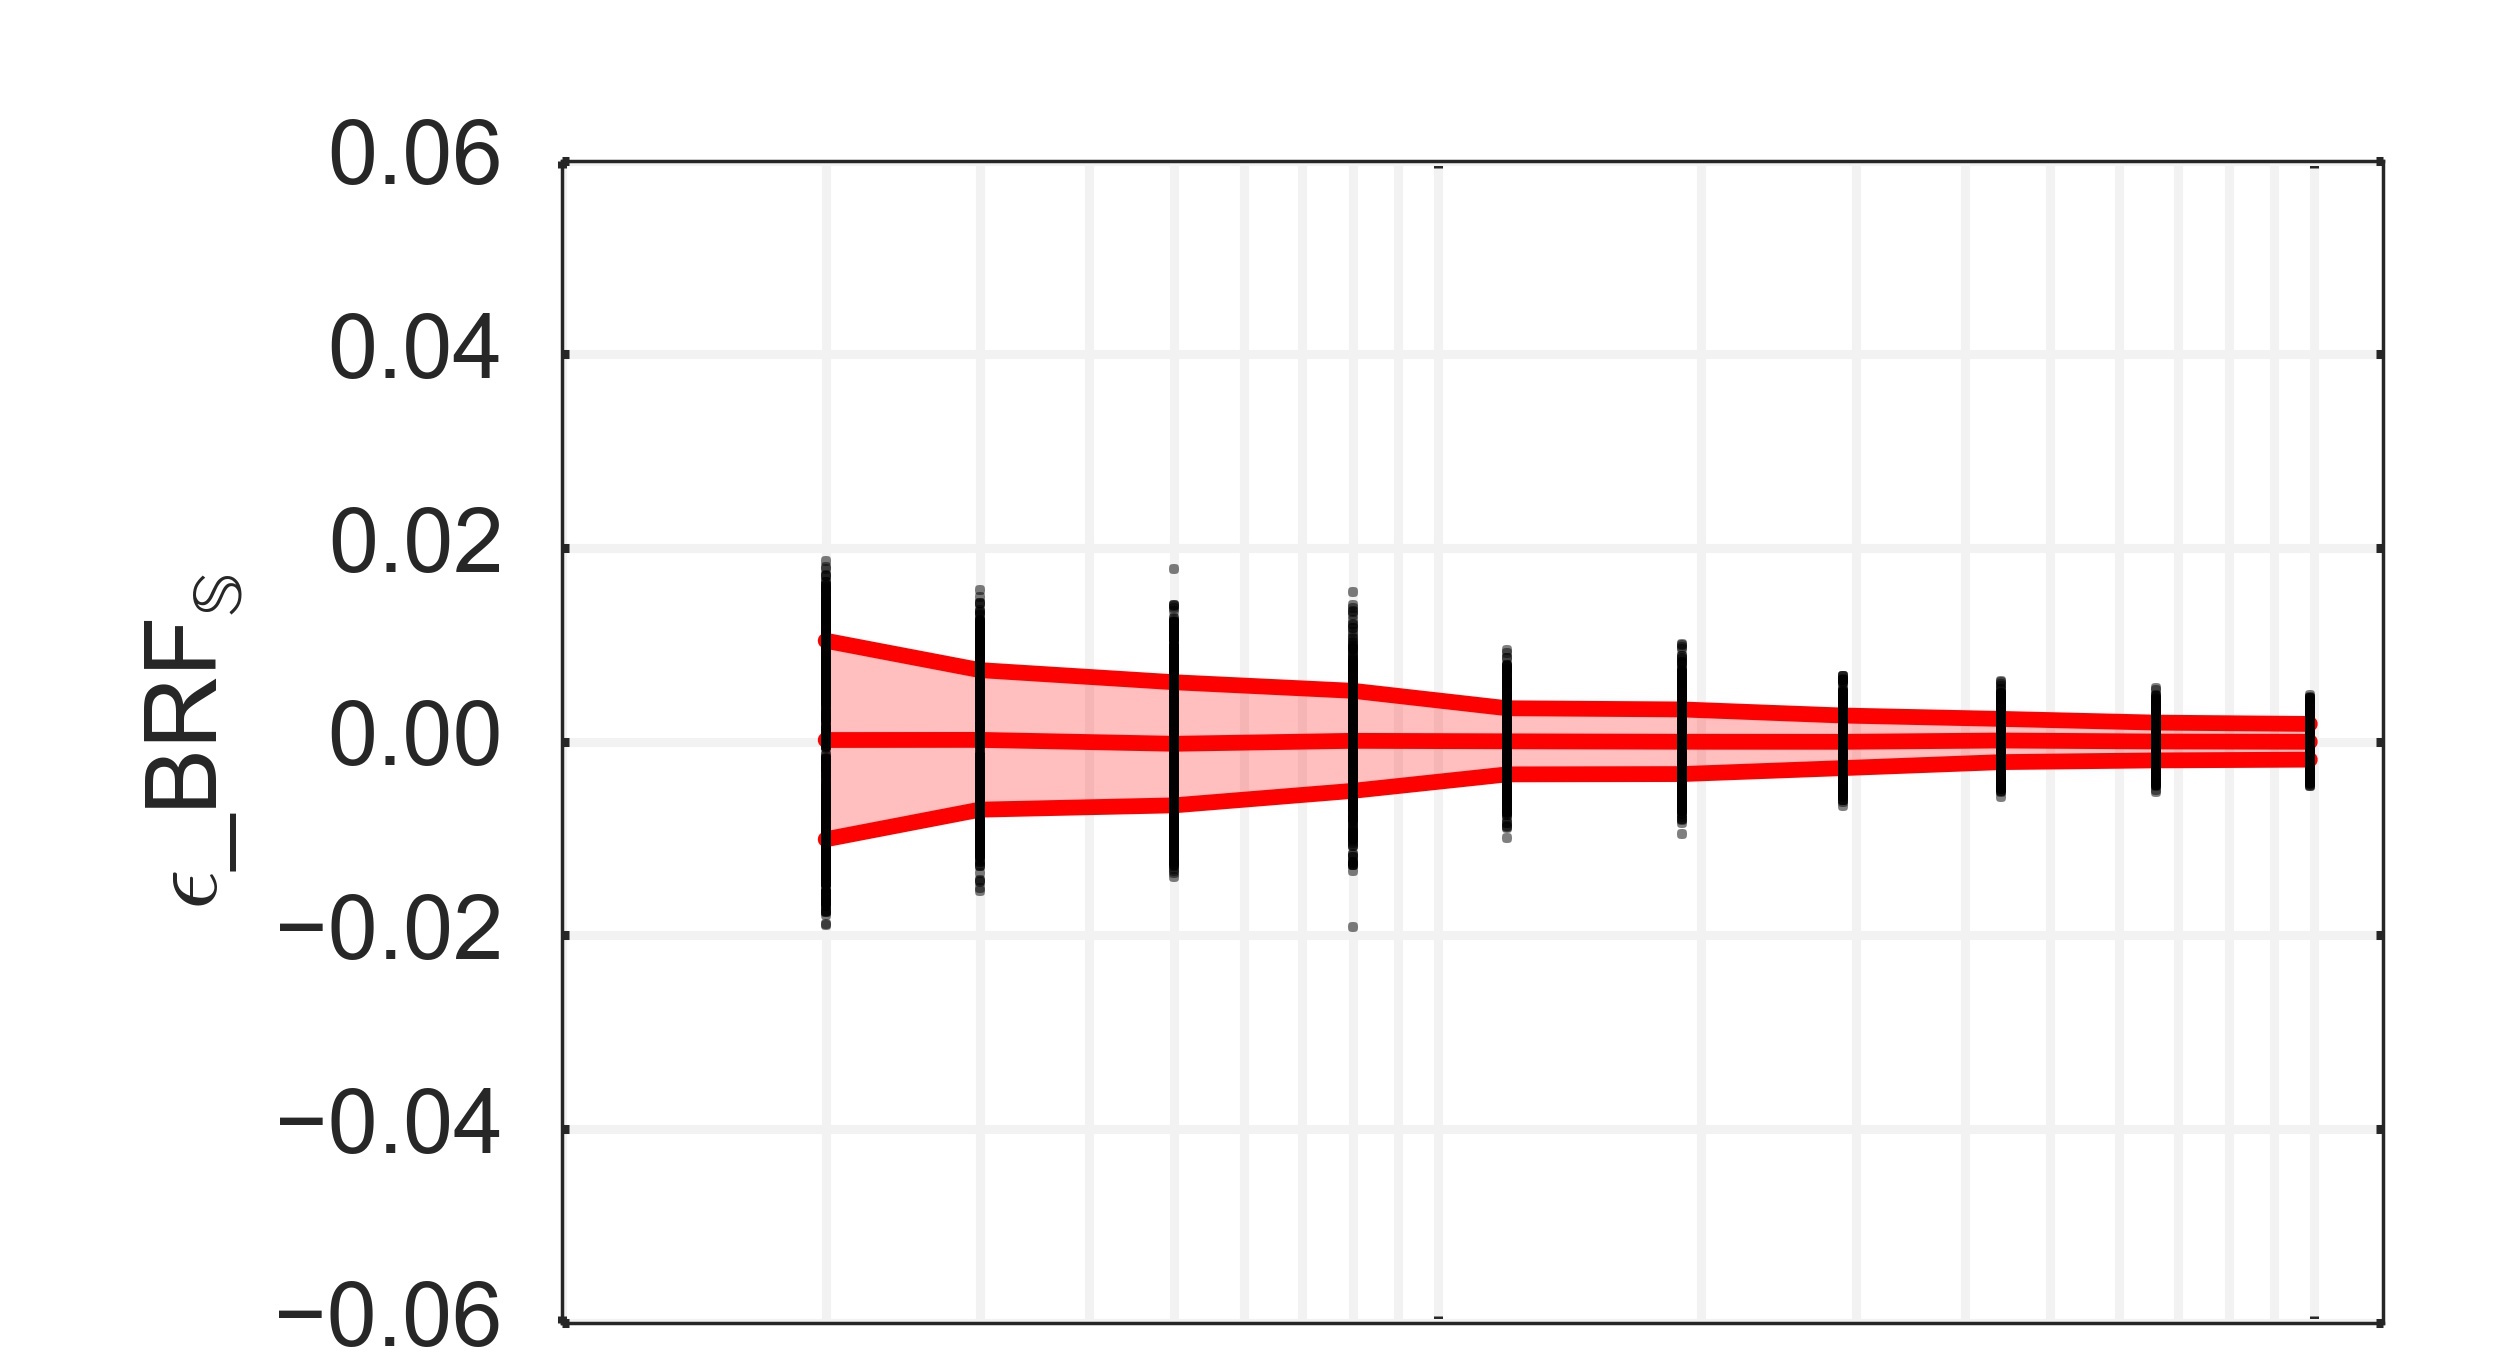
\includegraphics[width=0.32\columnwidth]{Figures/Convergence/CV_V_BRFBM_EFL_M12.jpg} \\
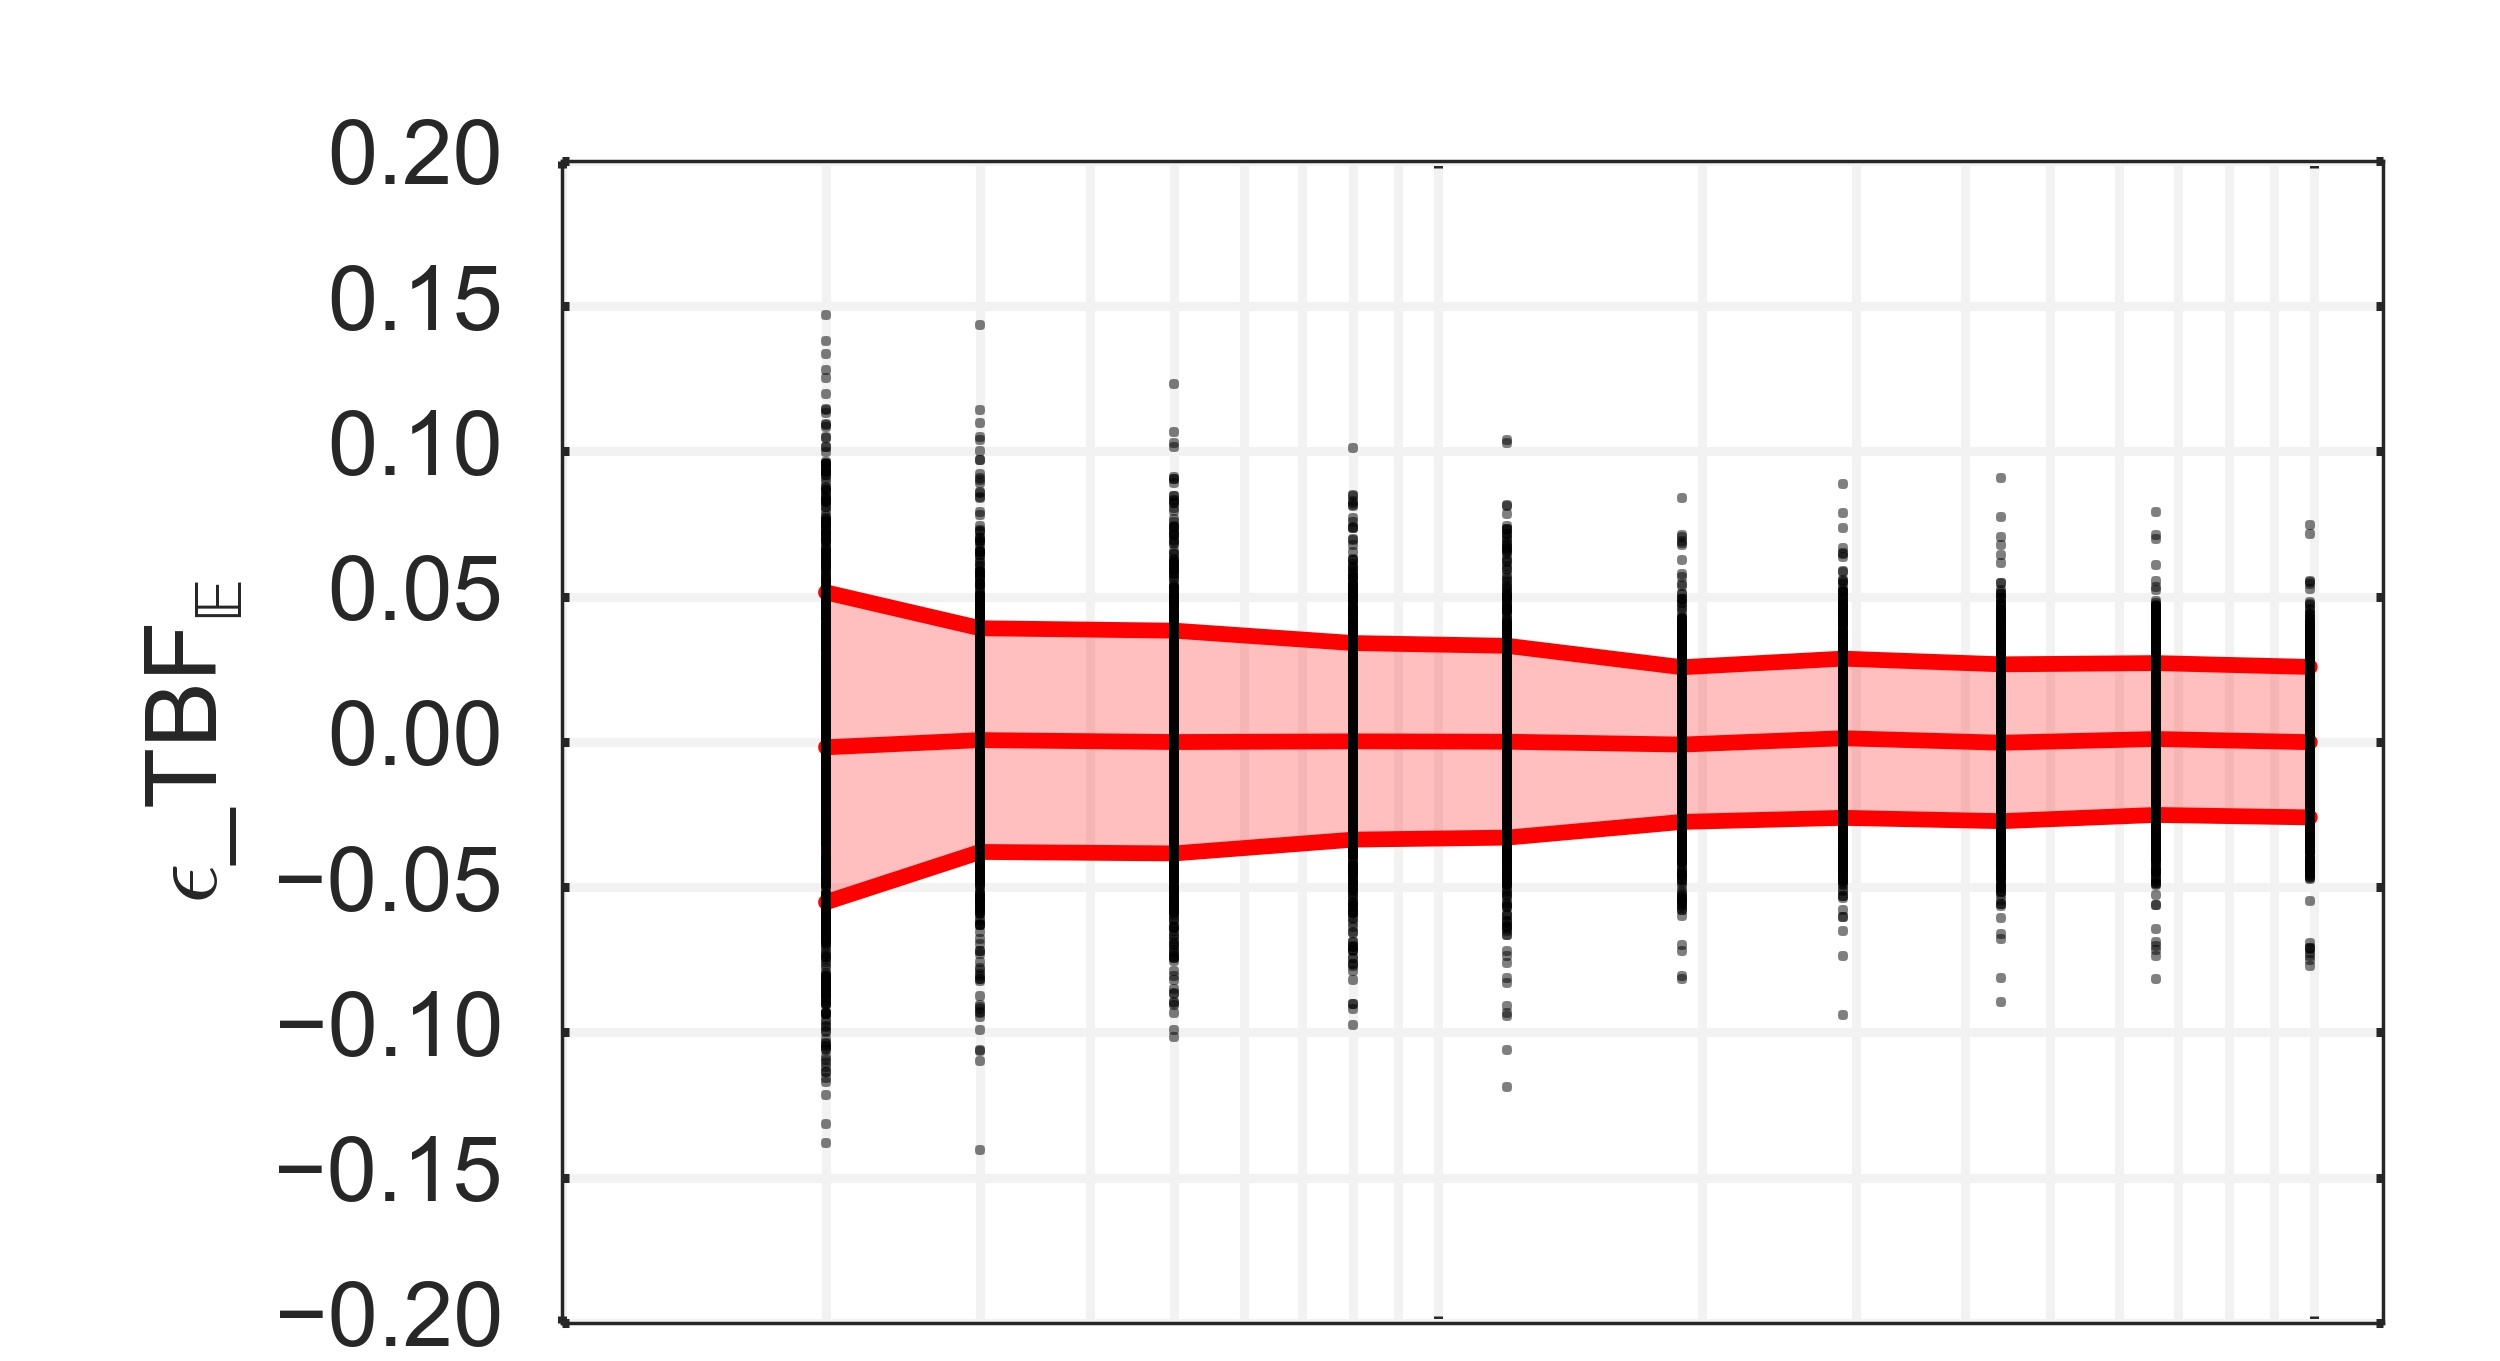
\includegraphics[width=0.32\columnwidth]{Figures/Convergence/CV_E_TBFBM_EFL_M4.jpg}
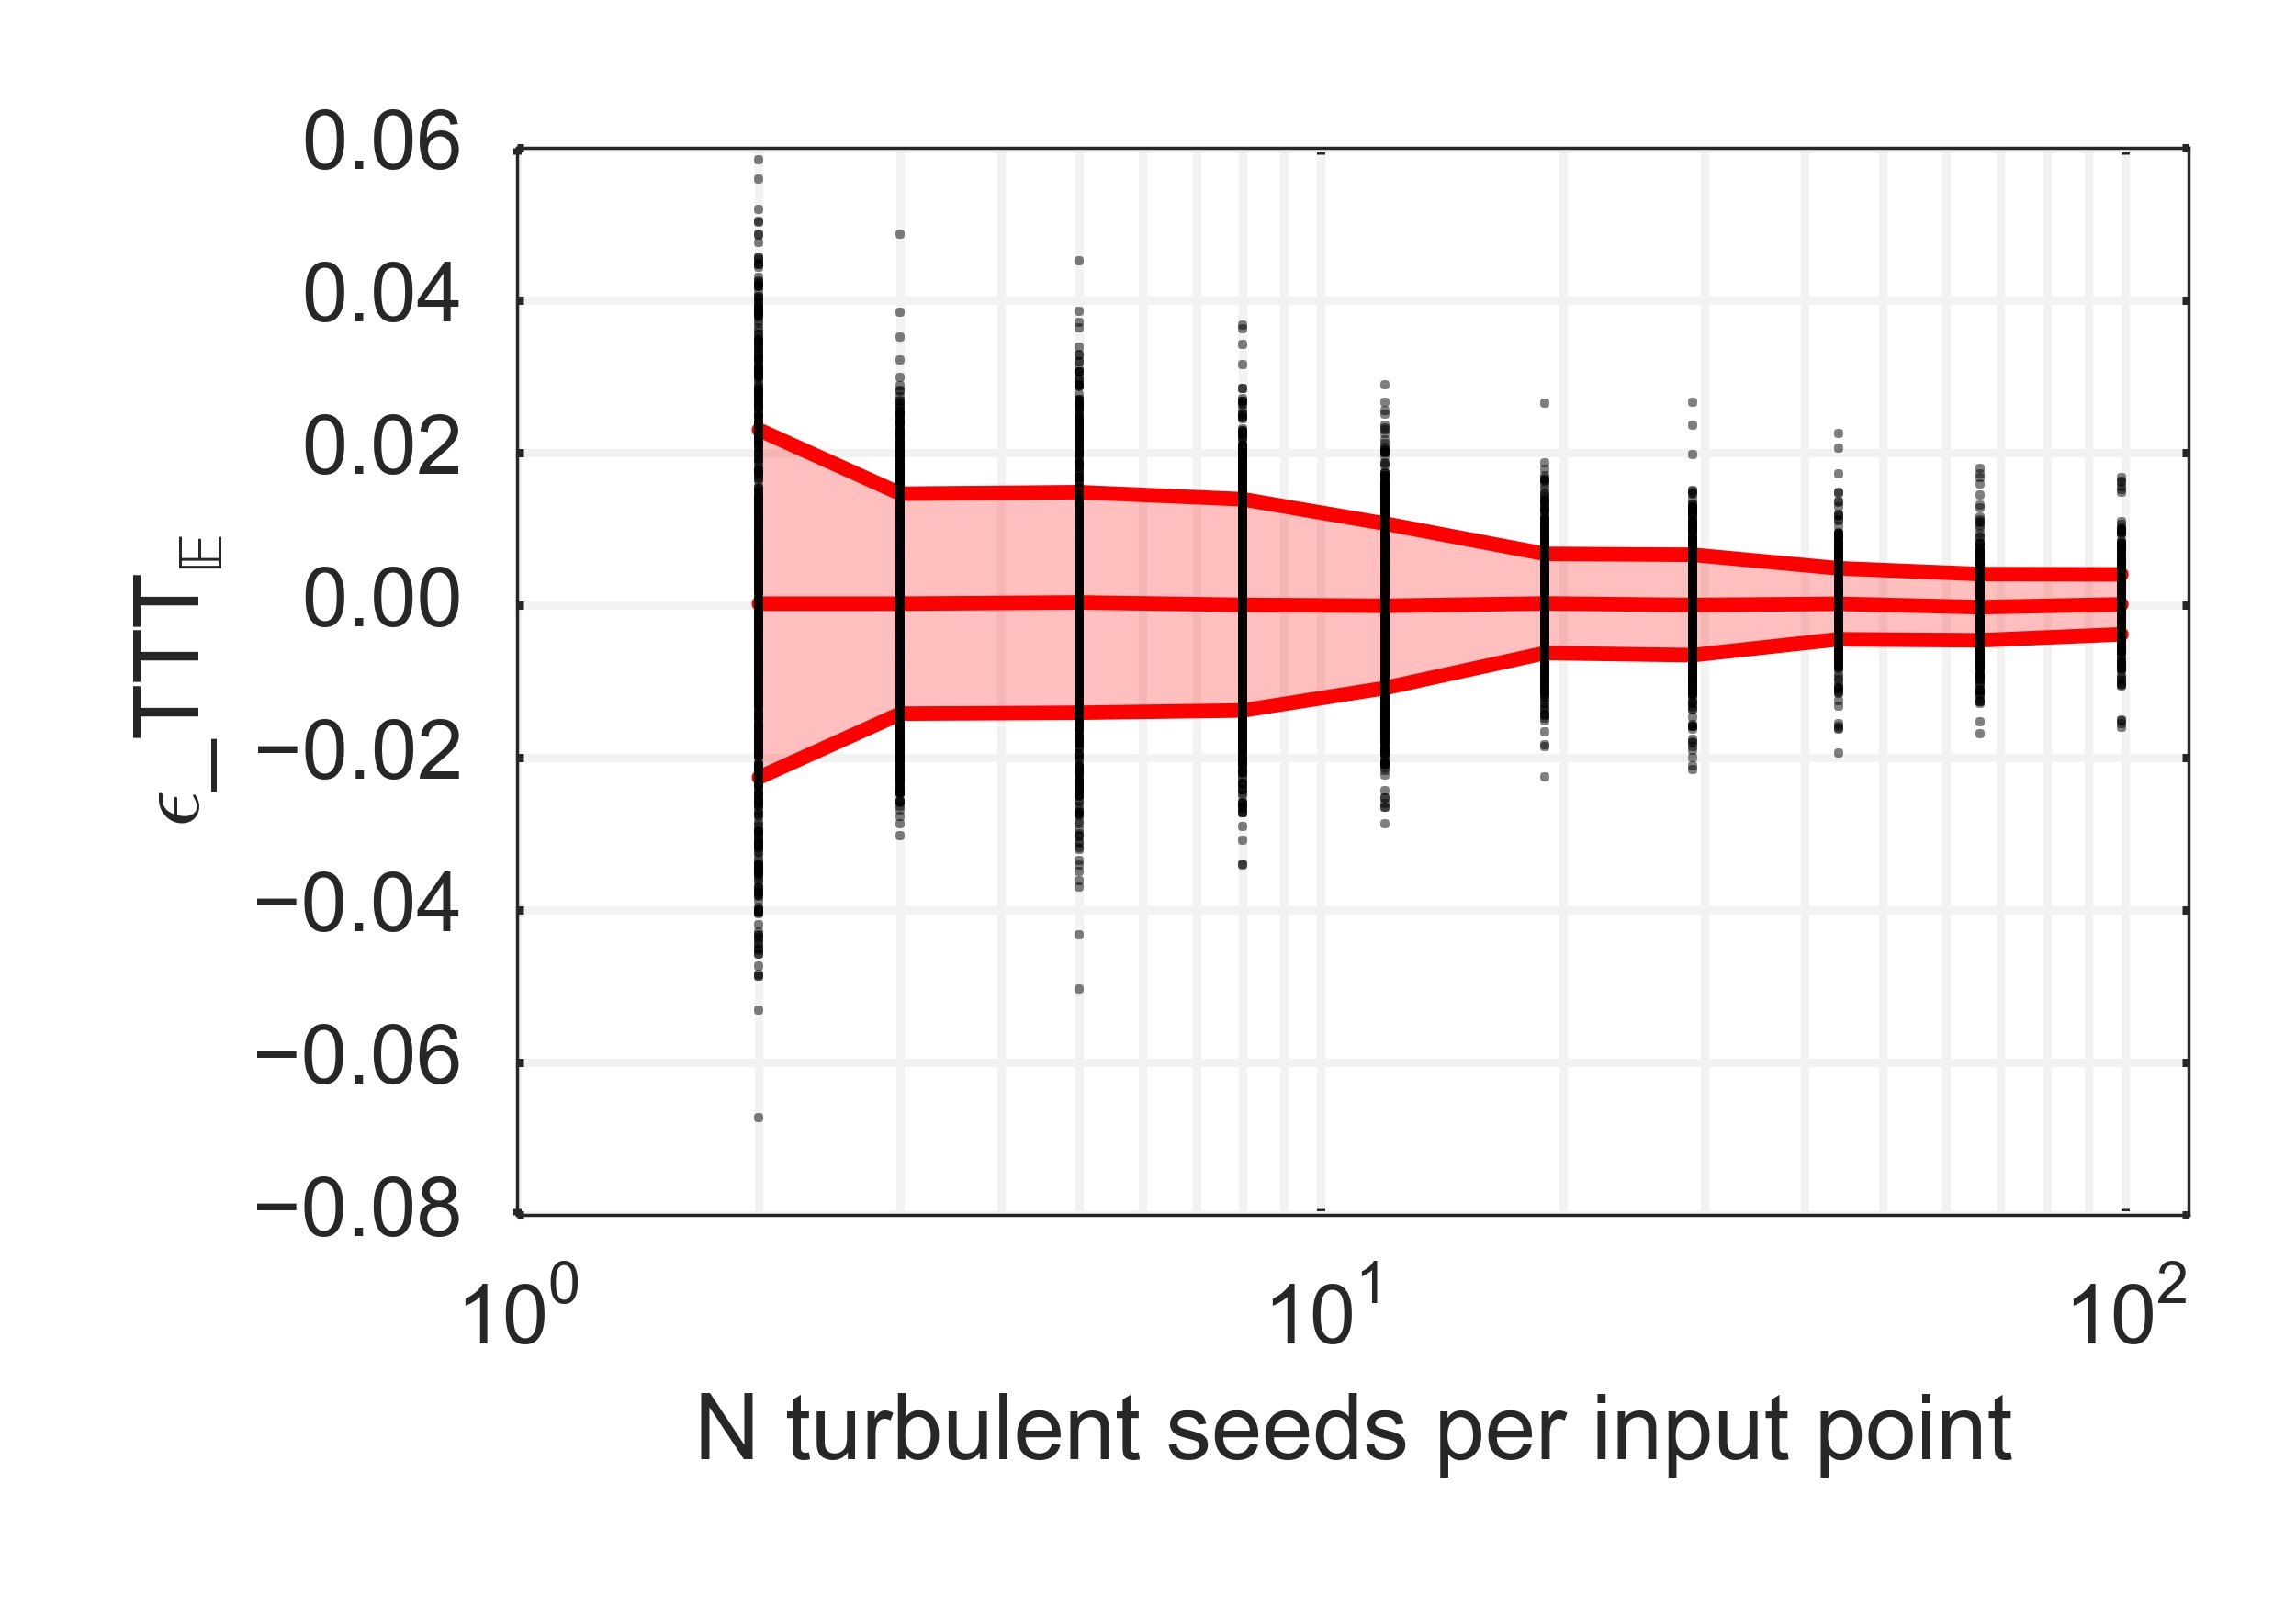
\includegraphics[width=0.32\columnwidth]{Figures/Convergence/CV_E_TTTBM_EFL_M4.jpg}
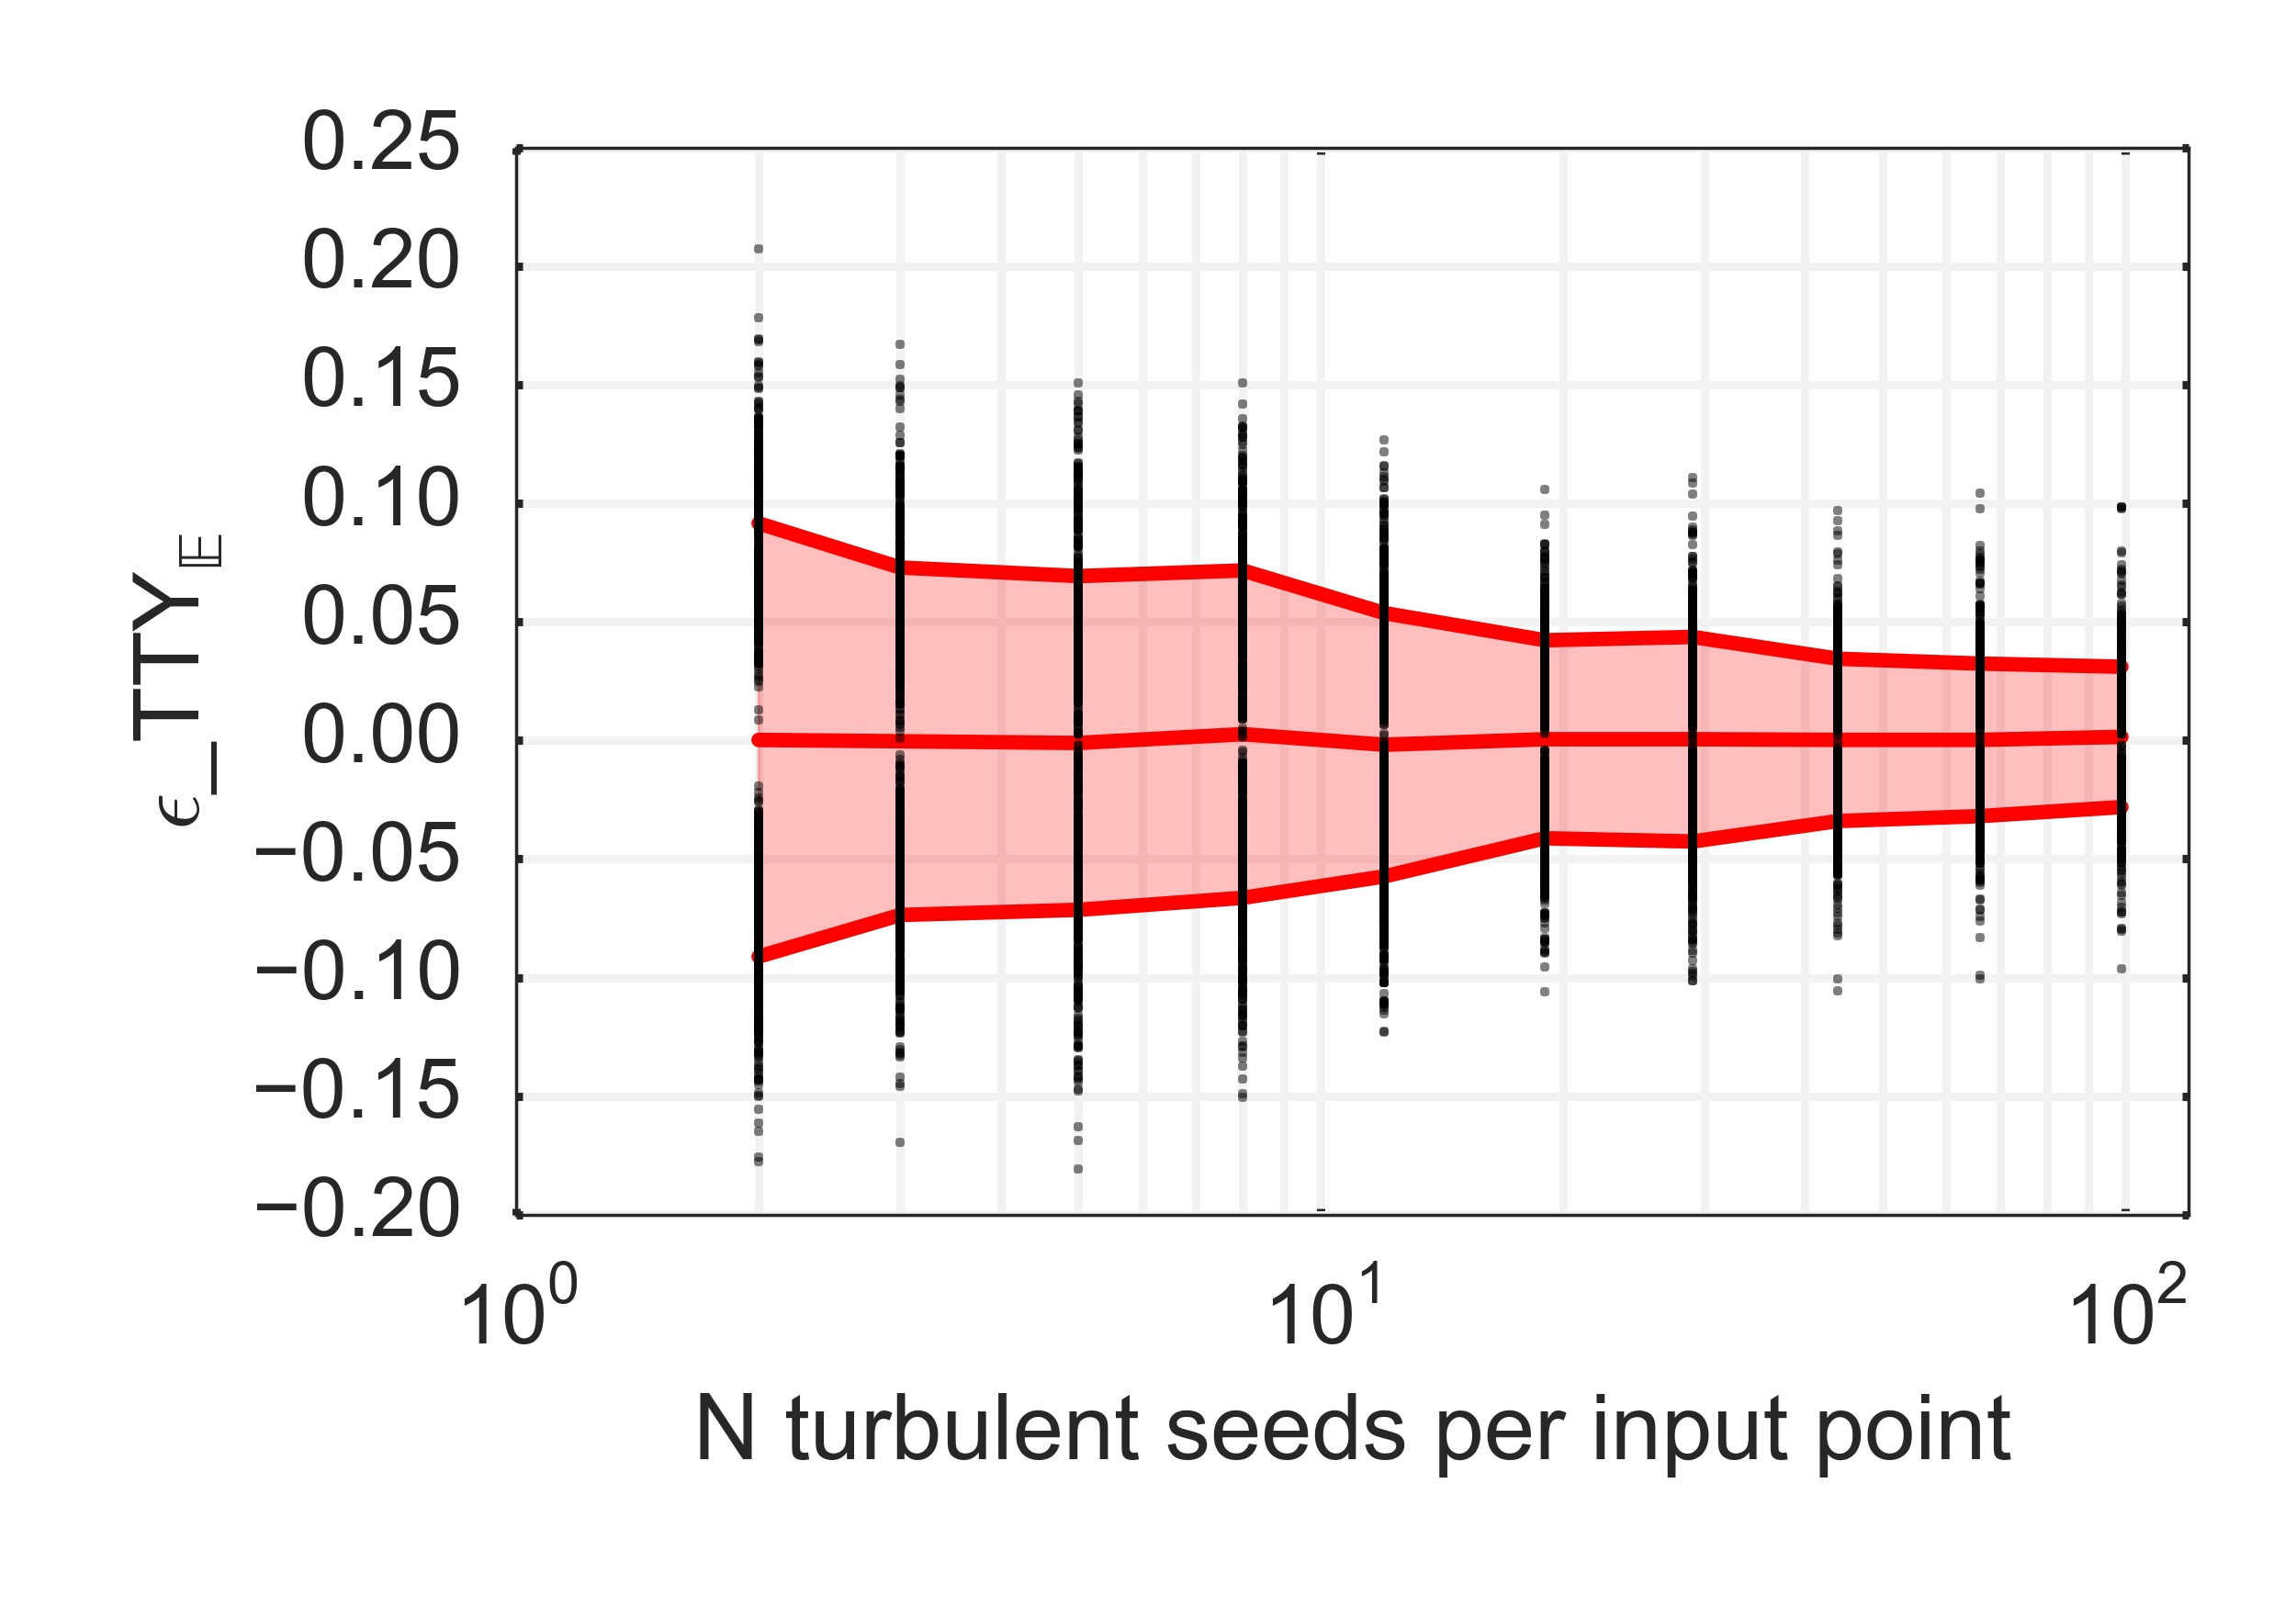
\includegraphics[width=0.32\columnwidth]{Figures/Convergence/CV_E_TTYBM_EFL_M4.jpg} \\
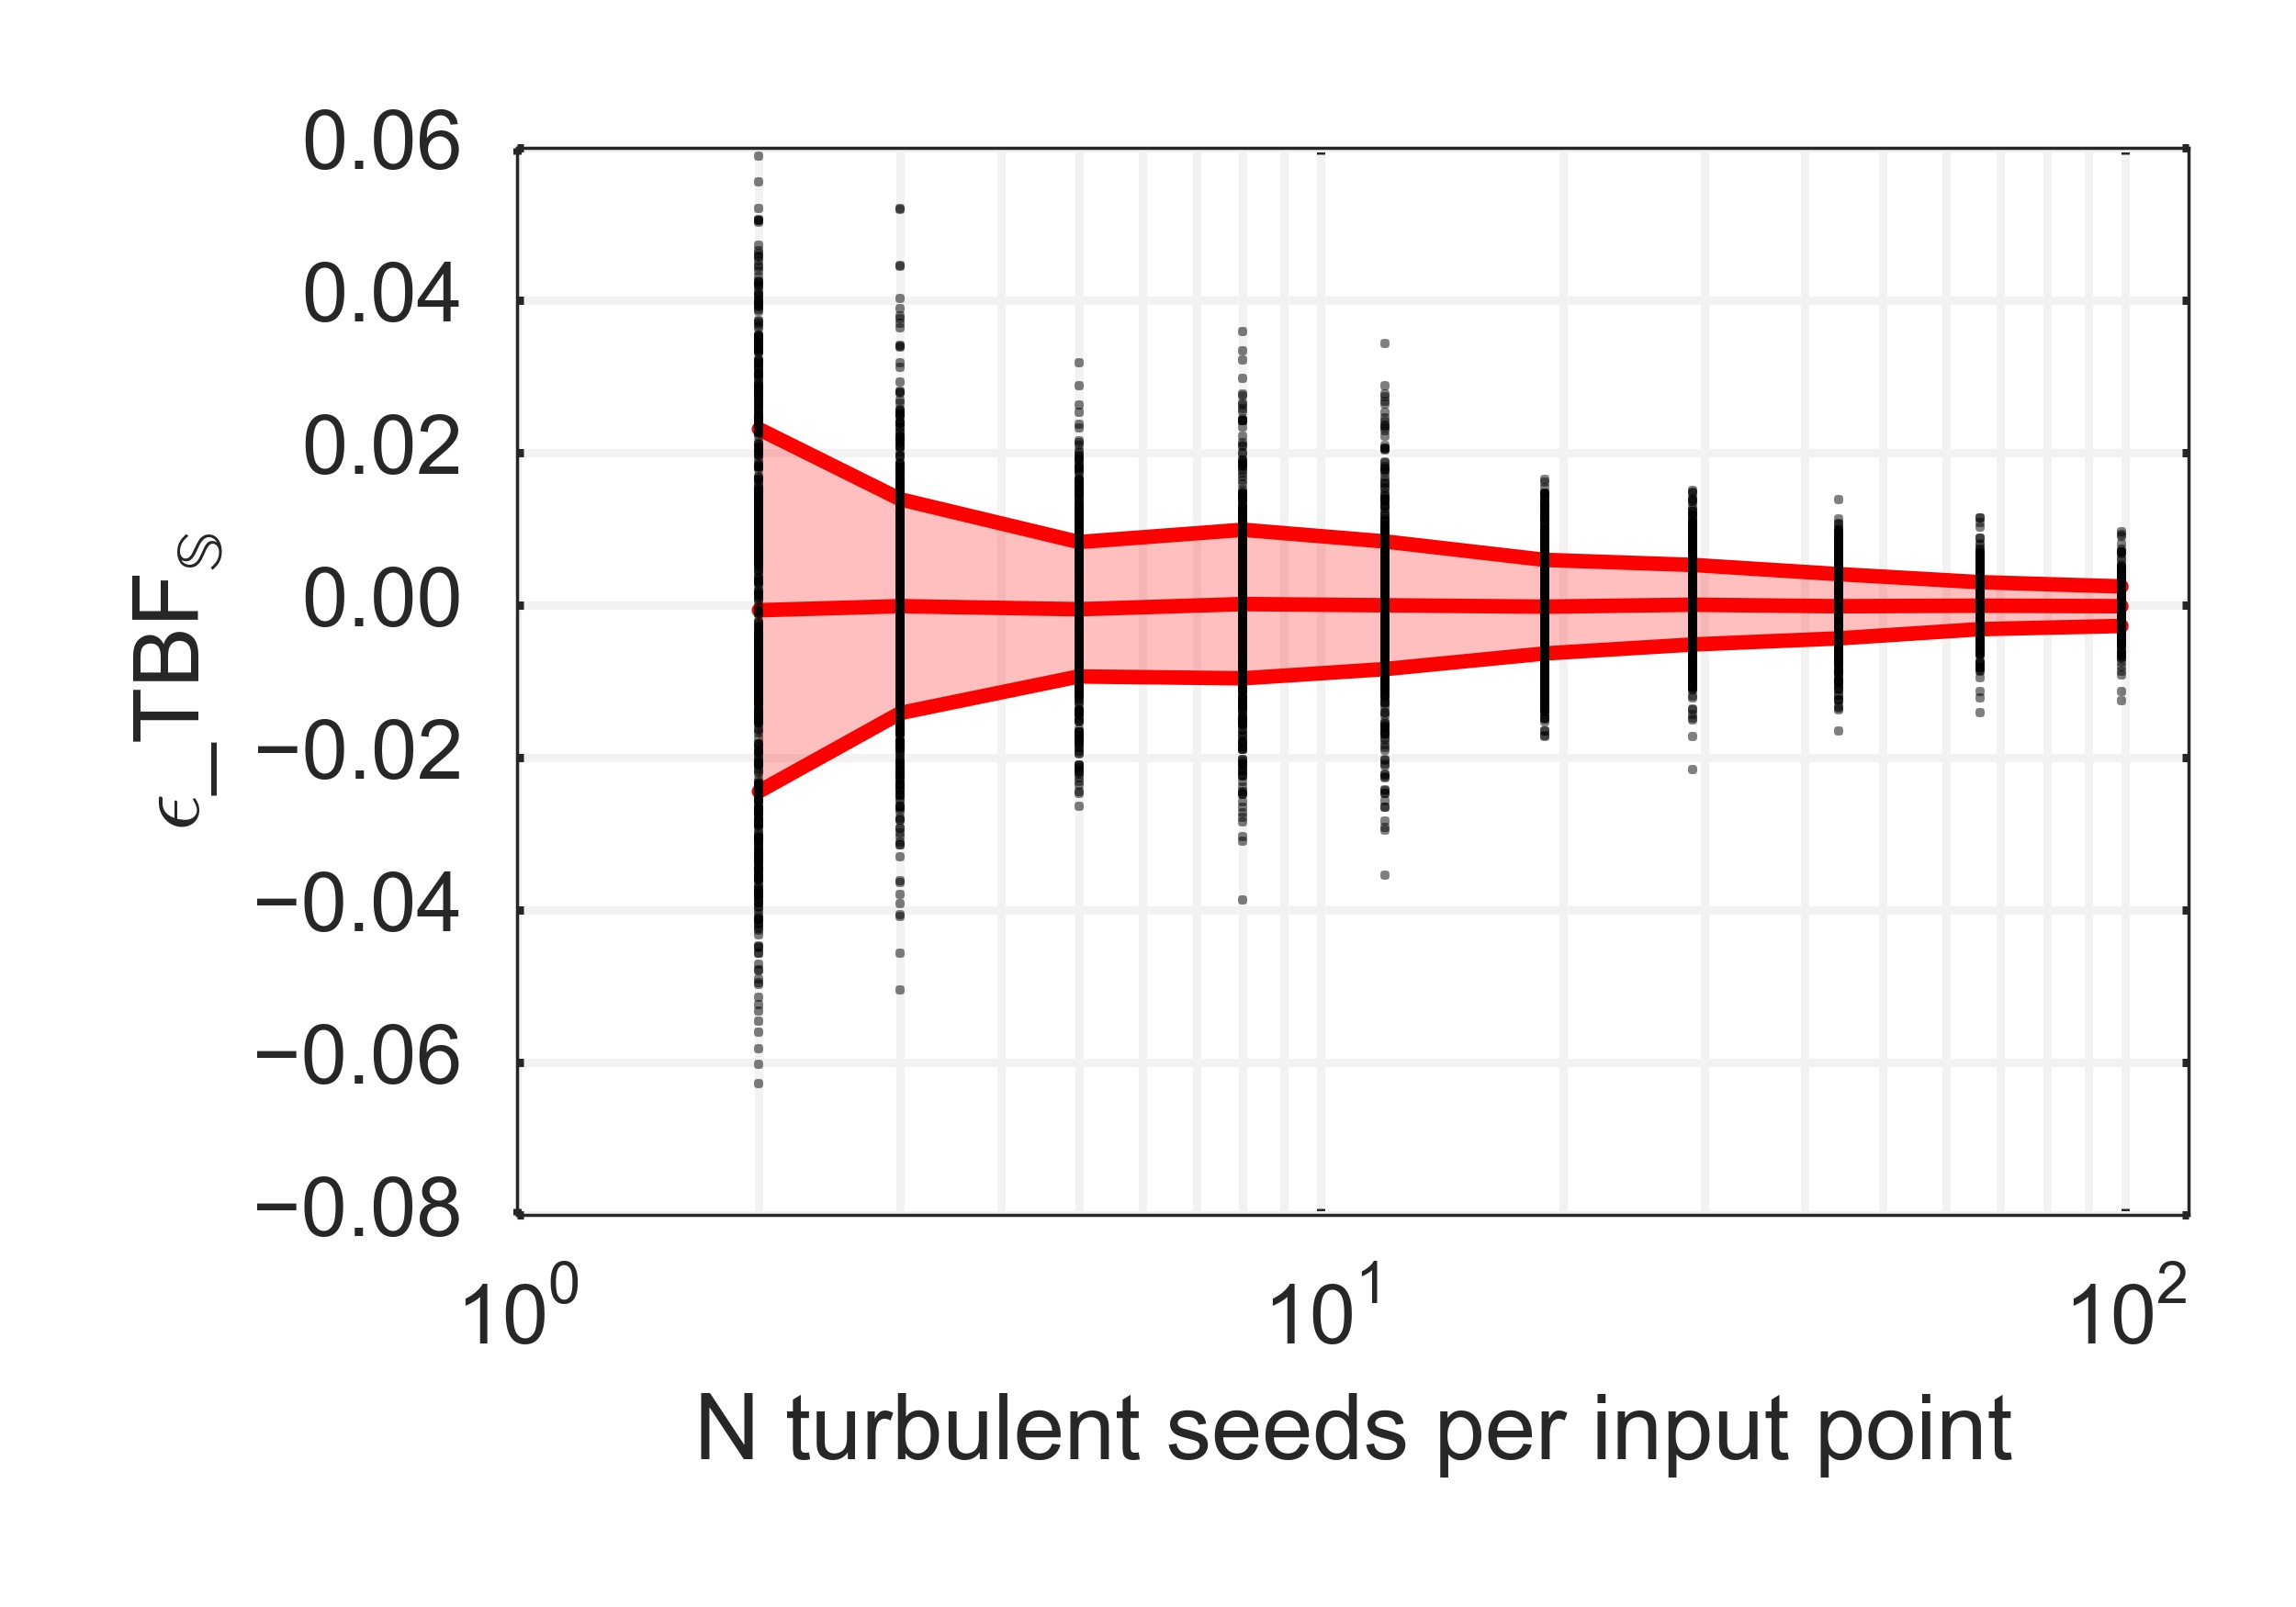
\includegraphics[width=0.32\columnwidth]{Figures/Convergence/CV_V_TBFBM_EFL_M4.jpg}
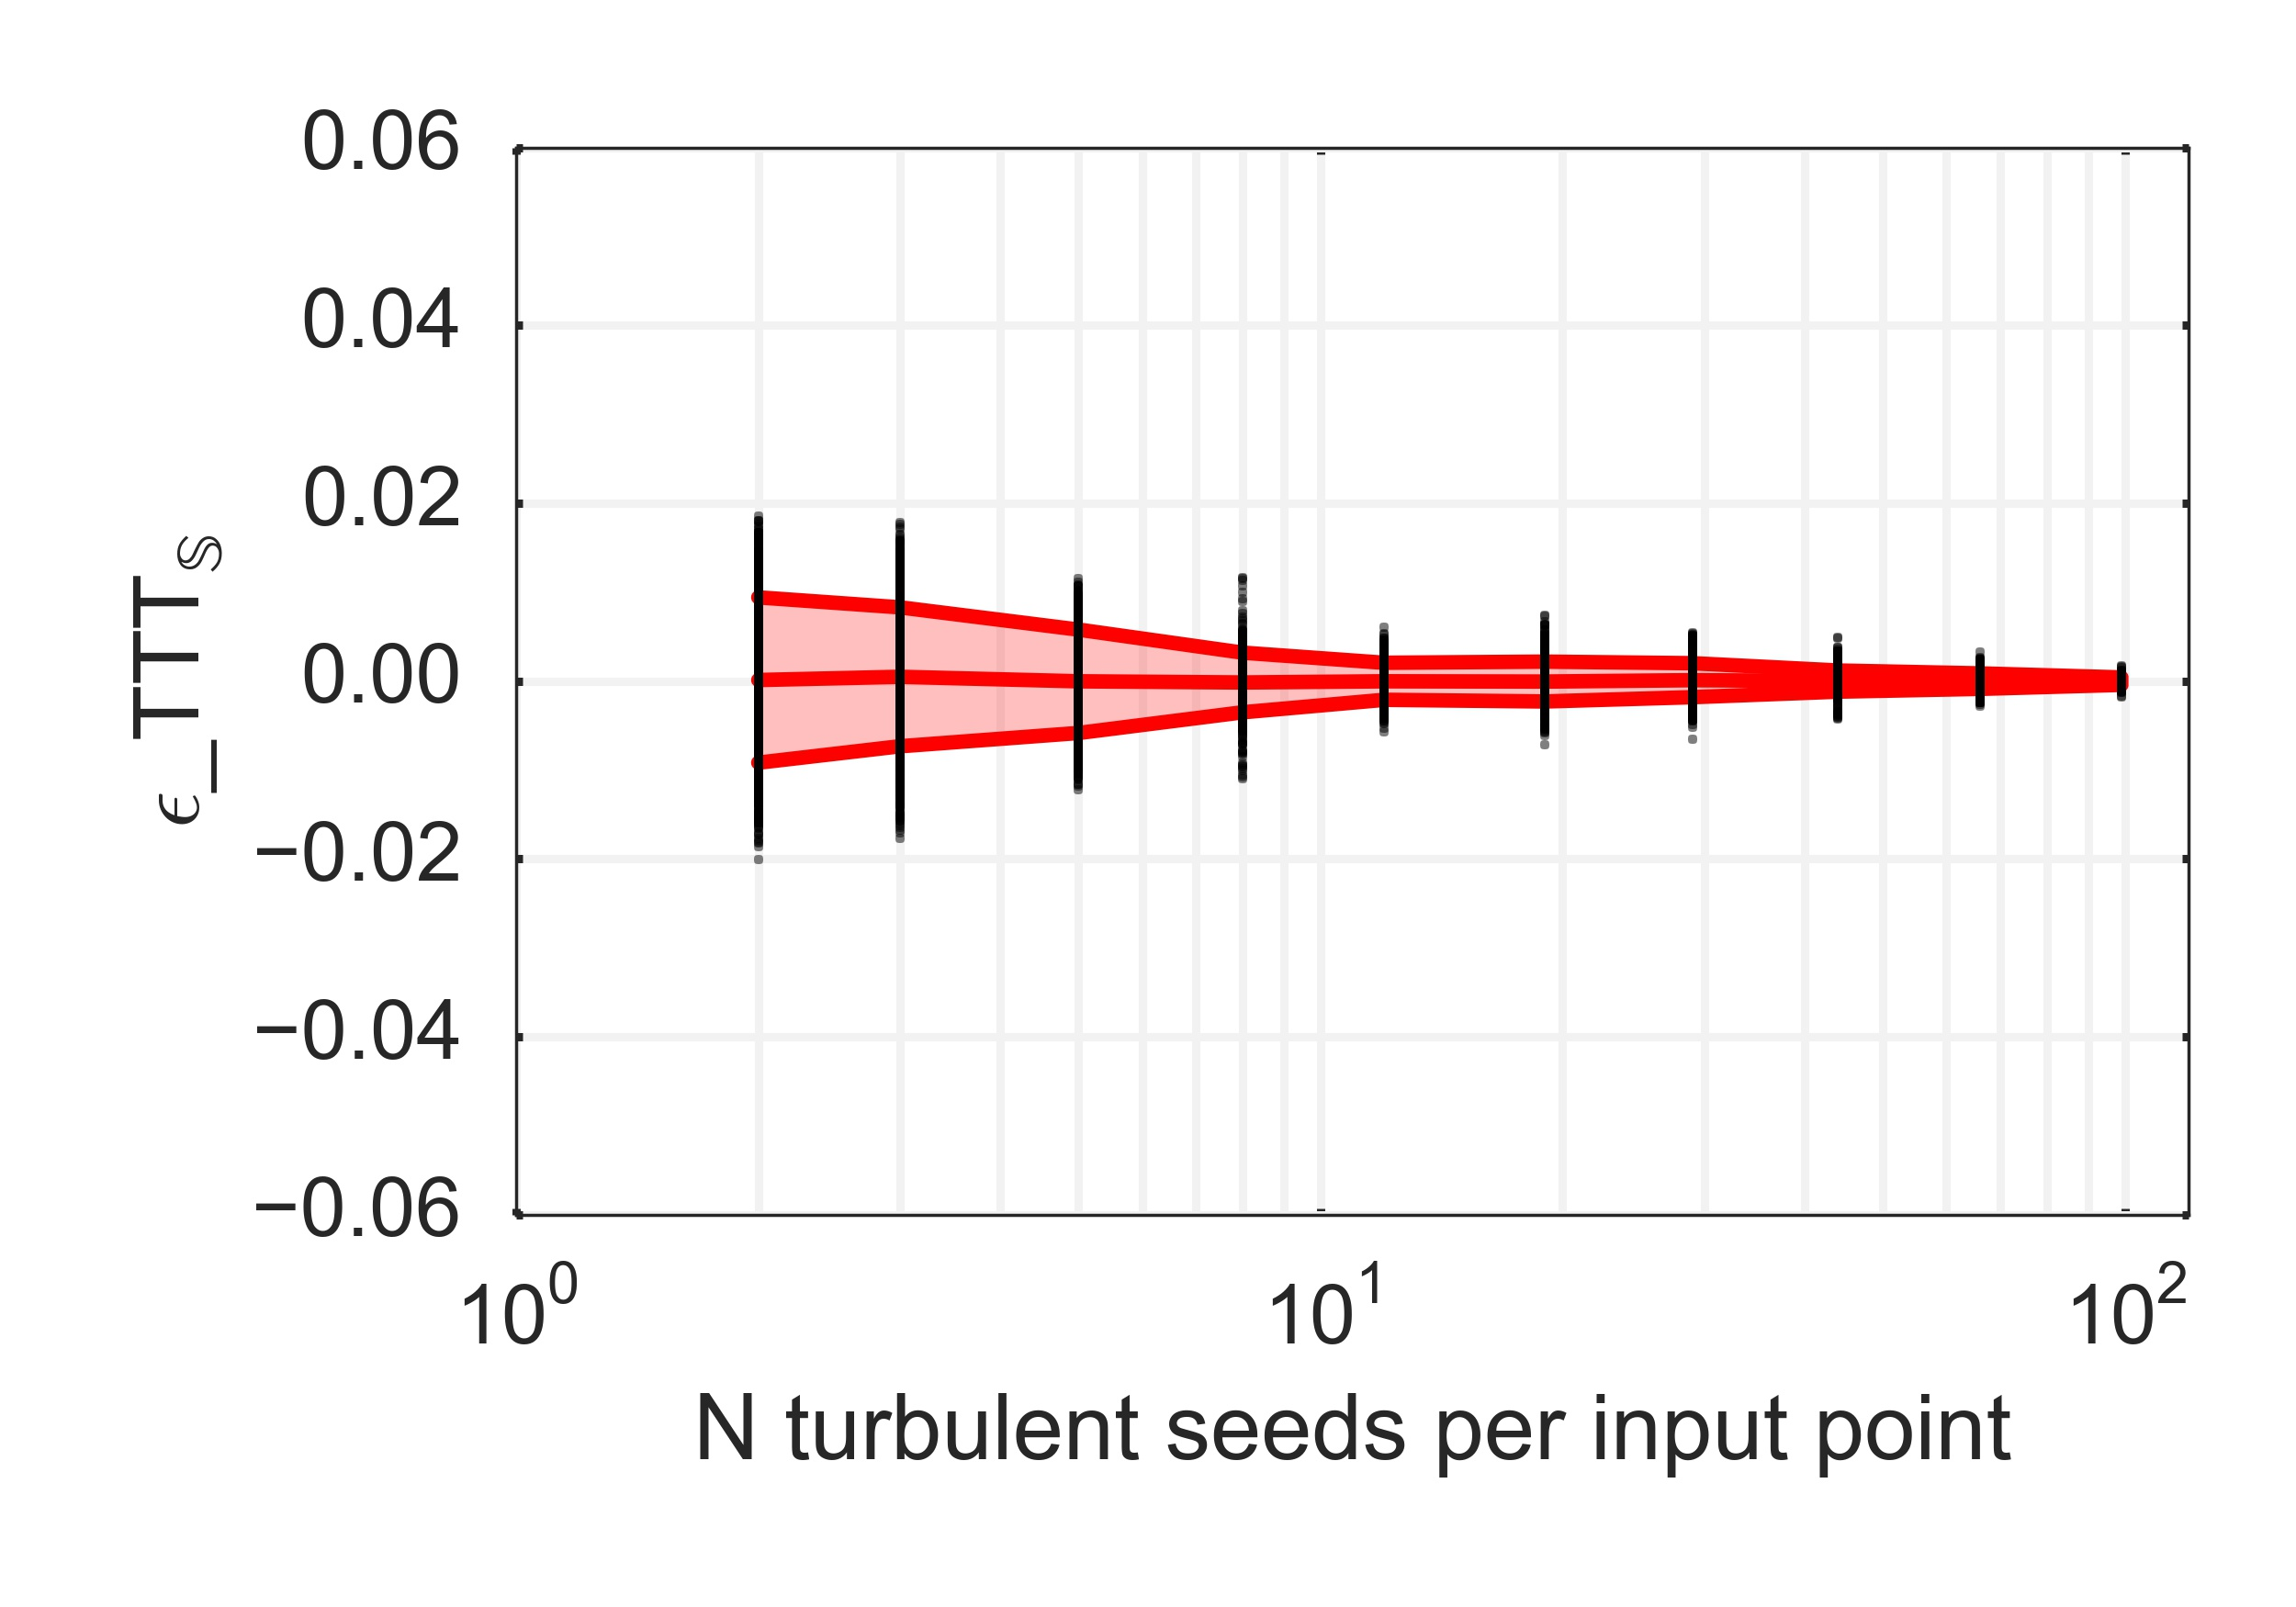
\includegraphics[width=0.32\columnwidth]{Figures/Convergence/CV_V_TTTBM_EFL_M4.jpg}
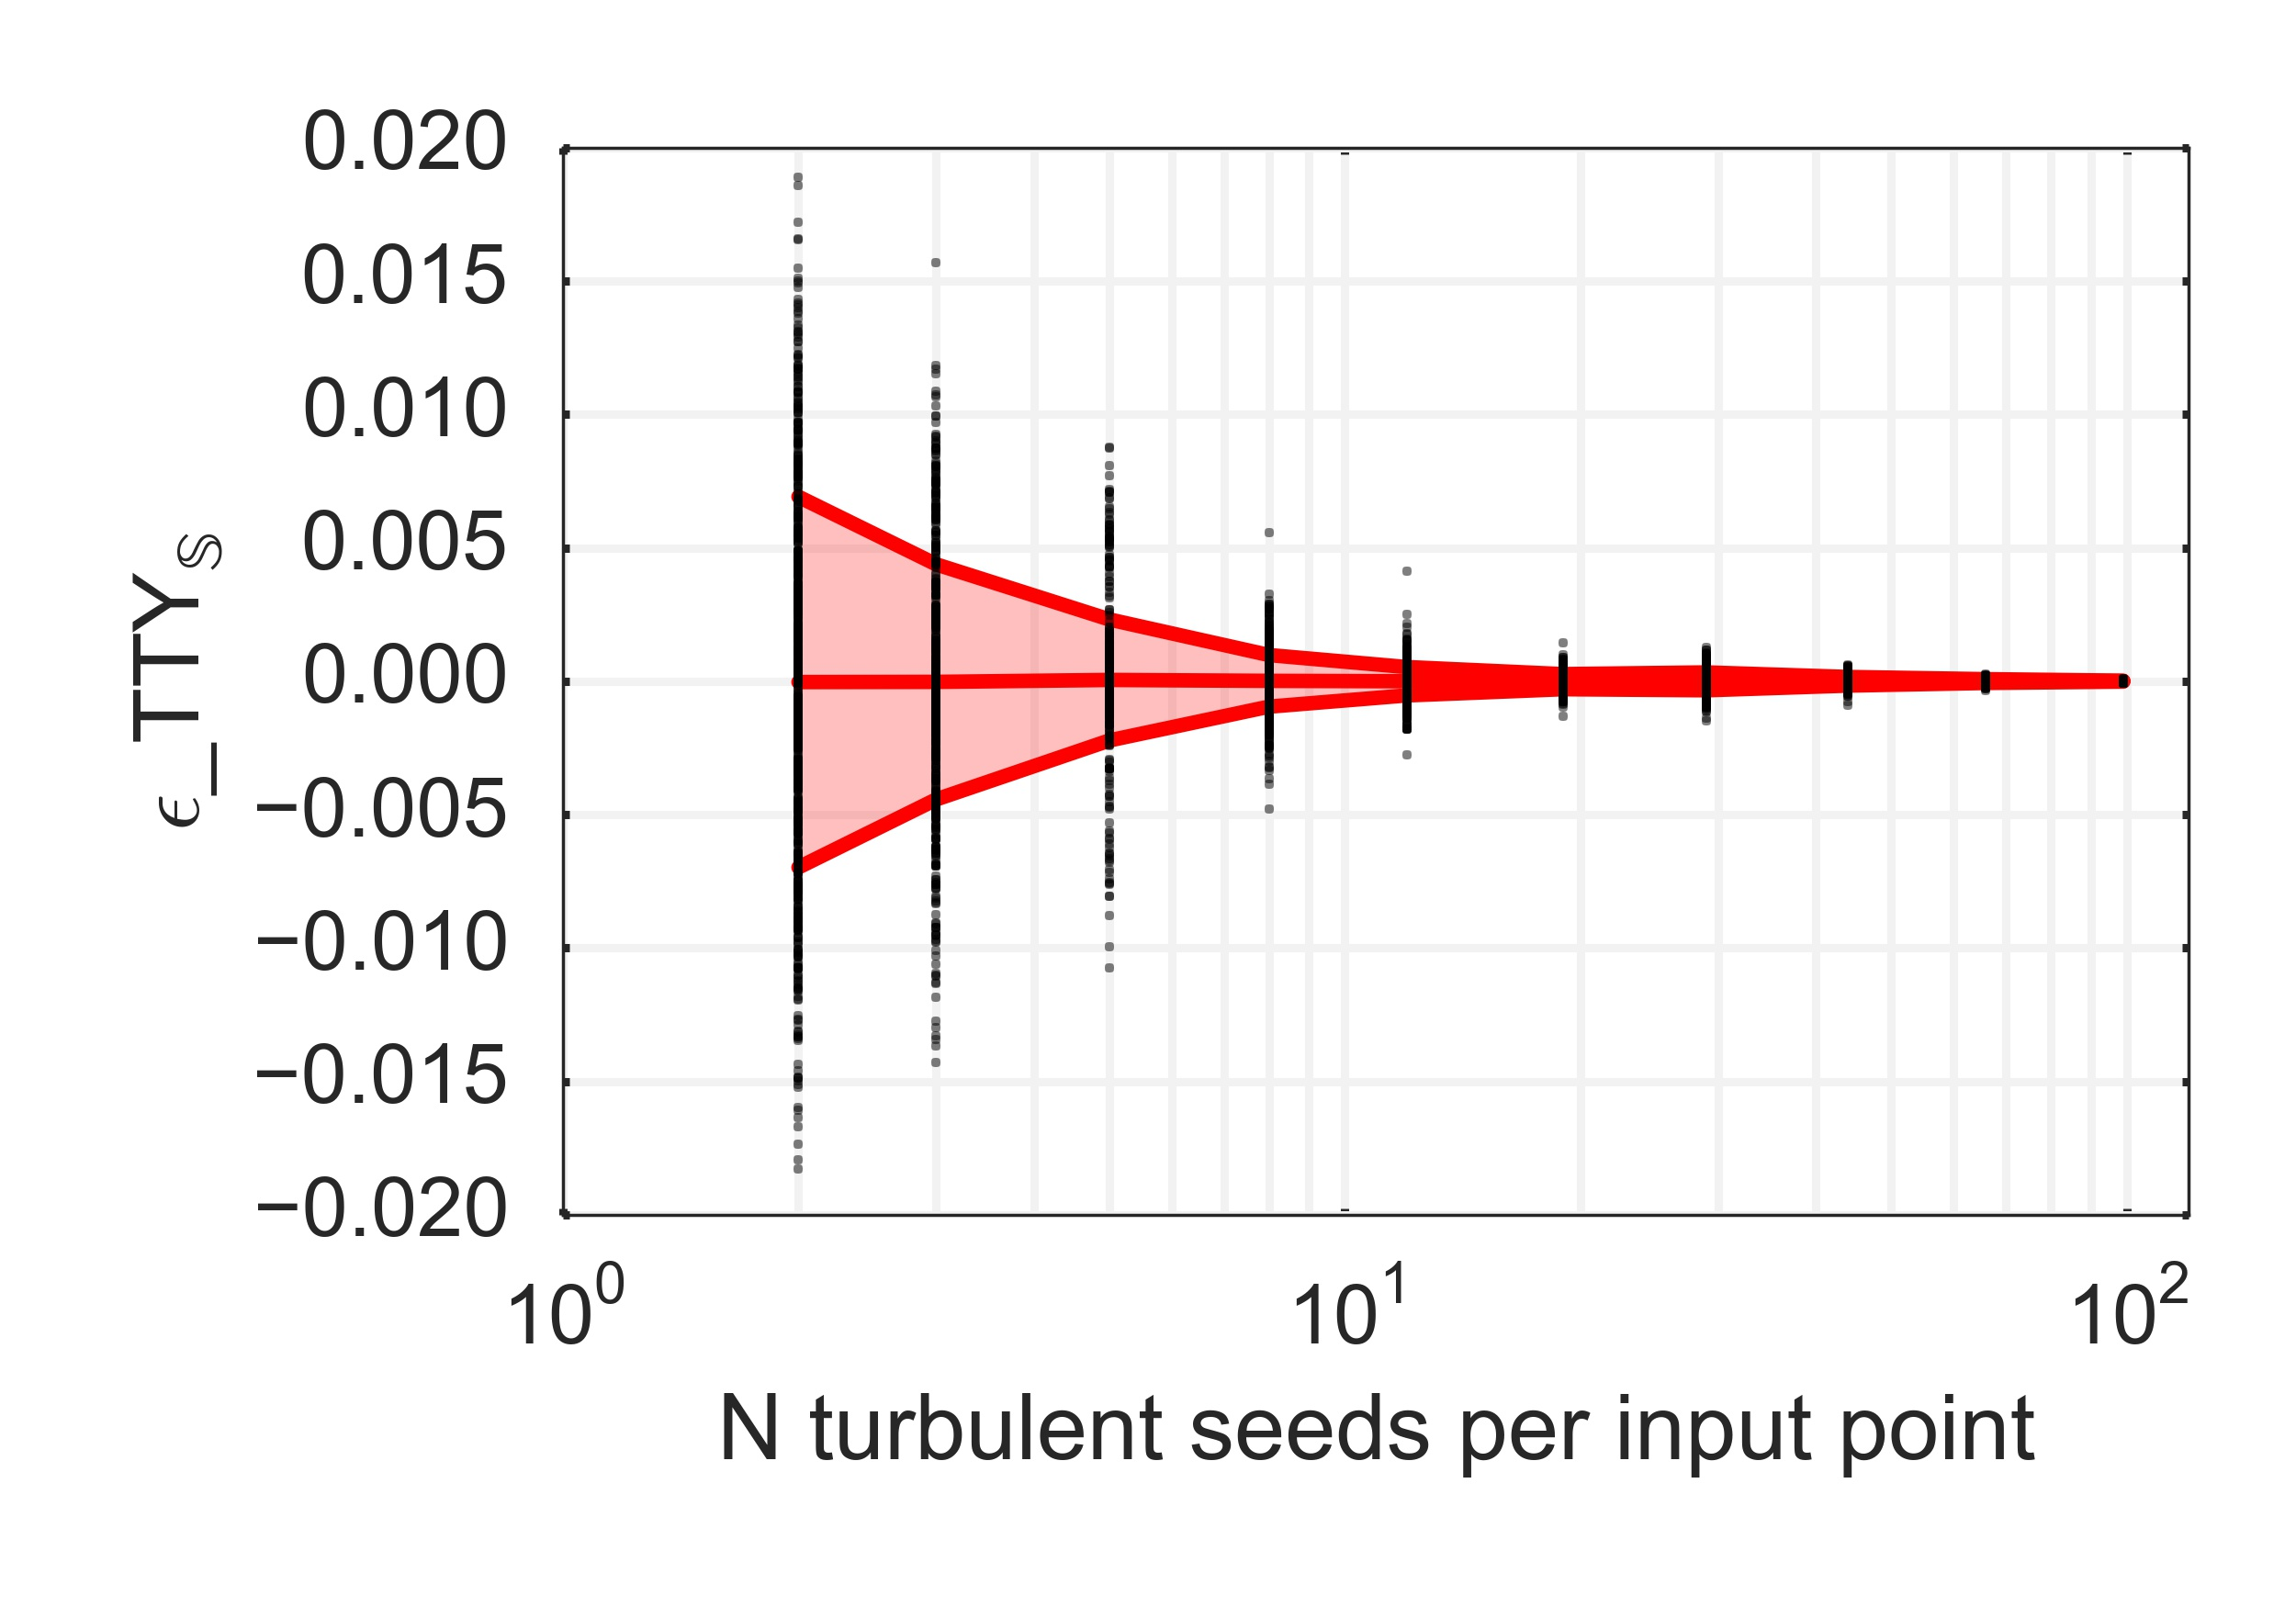
\includegraphics[width=0.32\columnwidth]{Figures/Convergence/CV_V_TTYBM_EFL_M4.jpg} \\
\caption{Convergence of the LOO cross-validation prediction error as a function of the number of turbulent seeds per input point used in PCE training. (Pink area) One standard deviation confidence interval around the mean $\expect(\epsilon) \pm \std(\epsilon)$.}
\label{fig_convergence}
\end{centering}
\end{figure}

% (Box plots) The horizontal lines that draw the boxplot represent Q1-1.5 IQR, Q1, median, Q3, and Q3+1.5 IQR. Where the inter quartile range is IQR=Q3-Q1, while Q1 is the 0.25 quantile and Q3 is the 0.75 quantile. (Black points) Outliers outside the interval [Q1-1.5 IQR, Q3+1.5 IQR].

\subsection{Example of using the surrogates for the estimation of the  uncertainty in annual energy production and lifetime equivalent fatigue loads}
\label{subsec_Final_EX}

This section presents an example to illustrate the use of the surrogates of the DTU 10 MW RWT to estimate the uncertainty in the yearly distribution of annual energy production and of equivalent fatigue loads. A single turbine is planned to operate in a location from which the yearly variability of wind resources has been studied during a long term (more than 20 years) campaign. The distribution of the variability of the wind resources is presented in the table \ref{tab_Unc_resource}. The main difference with the distribution used for training the surrogates is the fact that the $\ws$ follows a Weibull distribution with uncertain shape and scale parameters. This distribution of the Weibull parameters is used to characterize the year-to-year variability in the wind resources. Subsequently, the conditional distributions of $\stdws$, $\shear$ and $\yaw$ follow the same dependency described in the table \ref{tab_ins}.

\begin{table}[!h]
\begin{centering}
\resizebox{0.6\linewidth}{!}{
\begin{tabular}{cccc}
    \hline
    Variable & Distribution & \multicolumn{2}{c}{Parameters} \\
    \hline
    \\[-0.6em]
    $A$ & Normal & $\mu_A=9$ & $\sigma=0.5$ m/s\\
    \\[-0.6em]
    $k$ & Normal & $\mu_A=2$ & $\sigma=0.1$ \\
    \\[-0.6em]
    \hline
    \\[-0.6em]
    $x_0=\ws$ & Weibull & scale$=A$ & shape$=k$ \\
    \\[-0.6em]
    $x_1=\stdws$ & Lognormal & $\mu_{\stdws}(\ws)$ & $\sigma_{\stdws}(\ws)$ \\
    \\[-0.6em]
    $x_2=\shear$ & Normal & $\mu_{\shear}(\ws)$ & $\sigma_{\shear}(\ws)$ \\
    \\[-0.6em]
    $x_3=\yaw$ & Normal & $\mu_{\yaw}=0$ & $\sigma_{\yaw}= 5$ deg. \\
    \\[-0.6em]
    \hline
\end{tabular}}
\caption{Uncertainty in wind resources.}
\label{tab_Unc_resource}
\end{centering}
\end{table}

The propagation of uncertainty of this case is done in two steps. Initially a PCE with Gaussian quadrature is used to determine the nodes and weights of the distributions of the Weibull parameters $A$ and $k$, see equation \ref{eq_projection}. Each of these nodes represent the Weibull parameters in a given year. For each of these nodes, a large sample of the inputs of the surrogate, $\vx=[\ws, \stdws, \shear, \yaw]$, is generated. The size of the sample is the number of 10-min cases in a year: $365\times24\times6=52,560$ cases. The power and EFL are evaluated using the surrogate and the mean power and mean EFL for that year are calculated. Each individual surrogate evaluation has its own realization of the local distribution of the outputs due to the turbulence inflow realization, see equation \ref{eq_output_distrib}. Additionally, the effect of the errors of the surrogate can also be considered, by sampling the distribution of the errors for each evaluation of the outputs, see equation \ref{eq_output_distrib_U}. The results of the yearly distribution of capacity factor and of yearly equivalent loads are presented in figure \ref{fig_AEP_U}. There is no differences in the distributions of annual capacity factor or mean EFL obtained using the surrogate or the ones obtained including the uncertainty of the surrogate. The distribution in the capacity factor shows a negative skewness or a heavier tail for smaller values, which means that the p90 is smaller than the one predicted using a normal distribution. On the contrary, the annual distribution of mean TBF shows a positive skewness, which means that in certain years the accumulated fatigue damage for the tower can be much larger than average. The distribution of mean BRF is symmetric, but has heavier tails than a normal distribution.

\begin{figure}[h!]
\begin{centering}
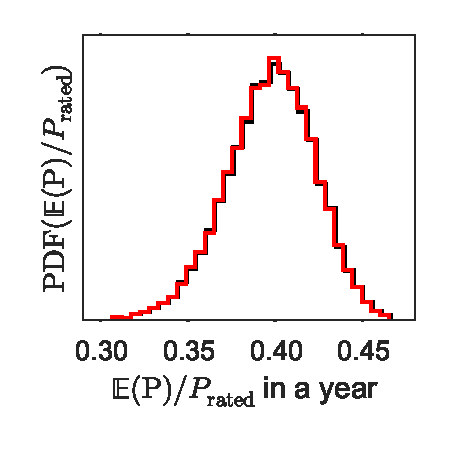
\includegraphics[width=0.32\columnwidth]{Figures/U_AEP/AEP_U.pdf}
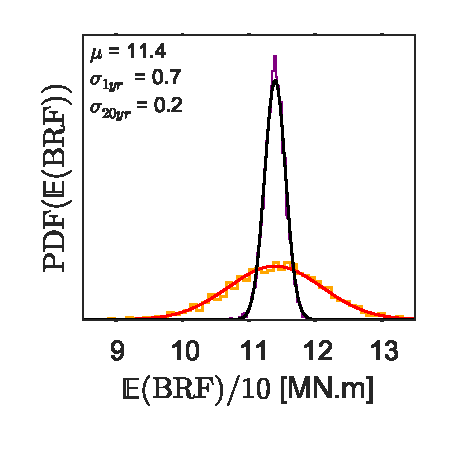
\includegraphics[width=0.32\columnwidth]{Figures/U_AEP/E_BRFBM_U.pdf}
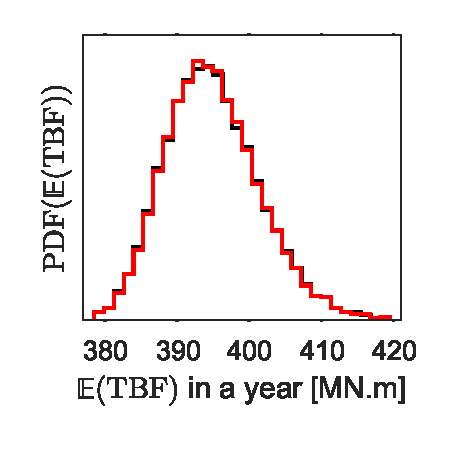
\includegraphics[width=0.32\columnwidth]{Figures/U_AEP/E_TBFBM_U.pdf}
\caption{Distribution of yearly distribution of capacity factor and of yearly BRF and TBF equivalent loads. (Black) Surrogate. (Red) Surrogate and surrogate prediction errors.}
\label{fig_AEP_U}
\end{centering}
\end{figure}


\section{Discussion}

The present article presents a methodology to implement sparse polynomial surrogates for aeroelastic wind turbine models. PCE are widely used in the uncertainty quantification field due to their efficiency to compute the statistical properties of the output and because the sensitivity analysis is obtained without any additional effort. The main two limitations in the use of PCE for wind energy are: (1) The input atmospheric parameters are usually jointly distributed with several layers of dependency (2) Some of the output have discontinuities and/or are restricted to certain values (e.g. only positive). The present article has shown how to solve this two problems: the implementation of an iso-probabilistic transformation to de-correlate the inputs, and  the use of a logistic transformation to implement restrictions on the outputs. The benefits of using the logistic transformation can be seen in figure \ref{fig_y_hat_E_V}, note that the PCE do not present oscillations in the constant regions, as it can be seen for P$_{\expect}$, for P$_{\std}$ and CT$_{\std}$.

The final surrogate can be used to generate an output sample that covers the full output space, and that will predict the general details of the distributions of the outputs. One of the main limitations of the present surrogates is that the local distribution of the output is assumed to be normal, this is not the case for the operating region close to rated wind speed. Since this assumption only affects the turbulent inflow realization, it is considered to be an acceptable approximation. The local distributions of most outputs are not normal in reality, because the wind turbine controller has different strategies in each operating region, which creates skewness in the local distributions.

The results presented in this article show that there are multiple dependencies between the input variables as well as between inputs and outputs. Such complicated inter-dependencies are difficult to capture when applying other methods such as interpolation or Gaussian processes. For example, advanced interpolation methods such as radial basis functions will not account for the likelihood of an extreme training point and will generate trends that always pass through all the model observations. This behavior penalizes the capacity of the surrogate to generalize and to predict the output in new conditions. The sparse PCE are ideal for this class of problems because the k-fold cross validation is a step inside the training. Additionally, the correlations between the outputs are fully captured when using the presented surrogates; this occurs because each of the outputs has a dependency on the inputs. The full pair plot of the training dataset and the resulting surrogate for all inputs and outputs is presented in the acompa. % What is "acompa"? I guess you have missed a few words in the end of this sentence.

The final results show a promising new approach to communicate the performance characteristics of a wind turbine between the turbine manufacturers and project developers. The wind turbine producers normally do not share the detailed structural and aerodynamic model information of their products due to intellectual property concerns. As a result, often the wind project planners and operators do not have the full information about the expected performance of a turbine at the site they are developing. Furthermore, typically there is no model for the uncertainty of the turbine performance. A possible application of the multiple polynomial surrogate could involve fitting the model by the manufacturer, and consequent distribution of the surrogate to users and clients. With this approach, project developers could get a useful tool for assessing site feasibility including uncertainty estimation, while not requiring access to detailed engineering models. Consequently, the use of more refined site assessment can potentially lead to improved overall estimation of levelized cost of energy and its uncertainty.

Obtaining the $\pdf(P)$ and $\pdf(EFL)$ is useful as they can be used for uncertainty estimation of the levelized cost of energy on a yearly basis. The surrogates can be evaluated on a long time series of the local wind resources (in multiple variables) such as the ones predicted by wind resource forecast (WRF) models without considerable extra computational effort. The power surrogate can then predict the annual variation of energy production while the EFL can be used to estimate the operation and maintenance costs. Such a probabilistic output can as an input to an e.g. decision support tool.

A surrogate of the DTU 10 MW RWT within a 4-dimensional turbulent inflow parameter space can be built using only 140 input cases (with multiple turbulent inflow realizations per case) and can be used to predict the distribution of the power, thrust coefficient and equivalent fatigue loads on the turbine. In contrast, traditional approaches require in the order of $20^4$ gridsearch/interpolation (full factorial design with  20 points per dimension) or $10^5-10^6$ variance reduction Monte-Carlo sample of the inputs \cite{dimitrov2015model}. Furthermore, the present approach enables to build an uncertainty model around the 10 minutes performance of the turbine that captures the effect of the turbulent inflow realization.

The combined PCE surrogate approach can also be used to improve traditional conservative designs in which a worst case scenario for shear and turbulence intensity is considered. The fast evaluation of the joint probability distributions for loads based on the surrogate model opens possibilities for performing structural reliability analysis and probability based design.

\section{Conclusions}

In the present study, a PCE-based polynomial surrogate model of wind turbine fatigue loads and energy output was defined and demonstrated for the DTU 10 MW reference wind turbine.
Using only 140 input cases was found to be sufficient for building a surrogate of the DTU 10MW model within a 4-dimensional turbulent inflow parameter space. The presented approach was demonstrated as an efficient alternative of the traditional techniques for characterizing the global behavior of an aeroelastic wind turbine model under multiple uncertain turbulent inflow parameters. % I've moved all the following paragraphs to the discussion - I think they belong there. In the conclusion, we should be more concise and concrete and outline the major findings from what we've done, not speculations on what this can be used for. So I would maybe add a few more sentences to the conclusion (e.g. the explained variance from Sobol indexes).
 
%% (This is a repetition of the discussion above)  The present approach can also be used to improve the estimation of the annual energy production and of the lifetime equivalent fatigue load based on site specific characteristics. The combined PCE surrogates can be understood as an extension of the power curve and can be a way to communicate the aero-elastic performance of a turbine between the manufacturer and the operators without compromising intellectual property. The final surrogate is an uncertainty model that predicts the performance of the turbine as a probability distribution for a given inflow condition. This uncertainty model of turbine performance can be easily implemented in different workflows such as: (1) Uncertainty quantification of the energy production inside a wind plant. (2) Robust wind plant layout optimization problem based on AEP and EFL and their corresponding uncertainties.

\section{Acknowledgments}

This work was supported by the International Collaborative Energy Technology R\&D Program of the Korea Institute of Energy Technology Evaluation and Planning (KETEP), granted financial resource from the Ministry of Trade, Industry \& Energy, Republic of Korea. (No. 20138520021140). The authors will like to thank Michael McWilliam for the suggestion of the use of logistic transformations to enforce strict restrictions to the polynomial surrogates.


%% The Appendices part is started with the command \appendix;
%% appendix sections are then done as normal sections
%% \appendix

%% \section{}
%% \label{}

%% If you have bibdatabase file and want bibtex to generate the
%% bibitems, please use
\section*{References}
\small
\bibliographystyle{elsarticle-num}
\bibliography{bib}

%% else use the following coding to input the bibitems directly in the
%% TeX file.

\begin{thebibliography}{00}

%% \bibitem{label}
%% Text of bibliographic item
%% \bibitem{}

\end{thebibliography}
%
%\appendix
%\section{Model selection - DTU 10 MW surrogate}
%
%Several number of folds are tested in the k-fold cross-validation selection of the proper level of sparsity in each of the outputs. 20-fold and 140-fold (maximum number of folds possible or leave-one-out) cross-validation results are shown in figure \ref{fig_20fold}. This figure shows the cross validation mean squared error for some of the outputs for all the possible training subsets. It can be seen that there is a large deviation in the errors when different folds are left for comparison. In particular, the extreme points in the input sample are important for the training process as they will contain the only information about the model response in regions with low probability. The error of a surrogate is larger if the training set does not include such extreme points. For the final results the 20-fold validation is selected because it gives a good balance between computational effort and accuracy in the estimation of the regularization coefficient obtained from %the leave-one-out.
%
%\begin{figure}[h!]
%\begin{centering}
%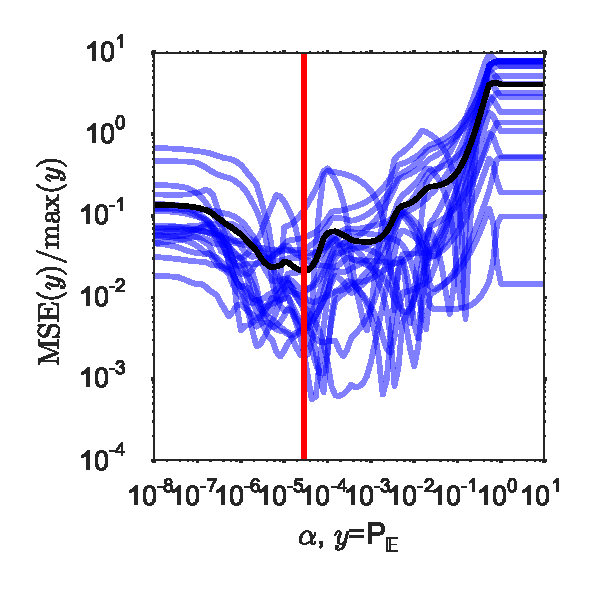
\includegraphics[width=0.32\columnwidth]{Figures/Surrgotes_20-fold/CrossValidation_P_E_PCE.pdf}
%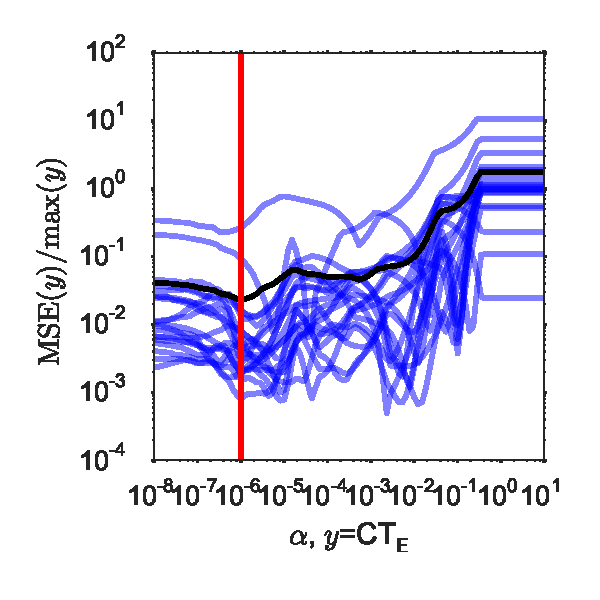
\includegraphics[width=0.32\columnwidth]{Figures/Surrgotes_20-fold/CrossValidation_CT_E_PCE.pdf}
%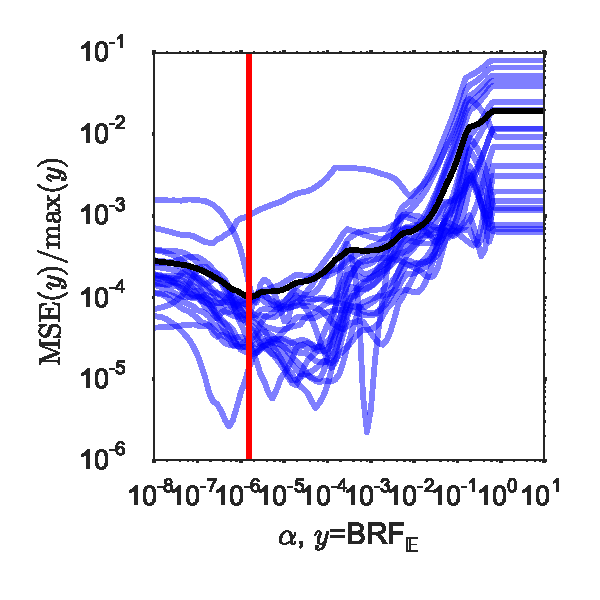
\includegraphics[width=0.32\columnwidth]{Figures/Surrgotes_20-fold/CrossValidation_BRFBM_EFL_M12_E_PCE.pdf} \\
%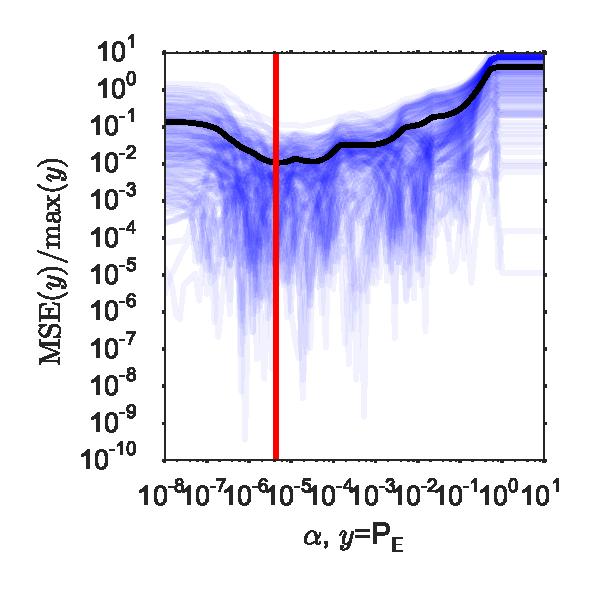
\includegraphics[width=0.32\columnwidth]{Figures/Surrgotes_140-fold/CrossValidation_P_E_PCE.pdf}
%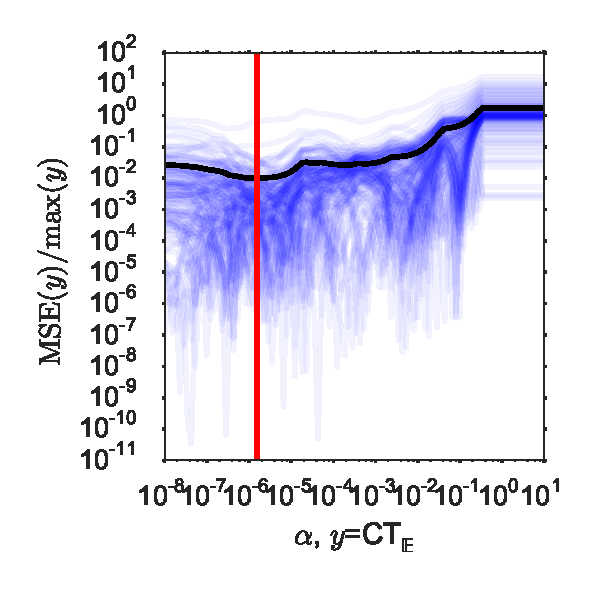
\includegraphics[width=0.32\columnwidth]{Figures/Surrgotes_140-fold/CrossValidation_CT_E_PCE.pdf}
%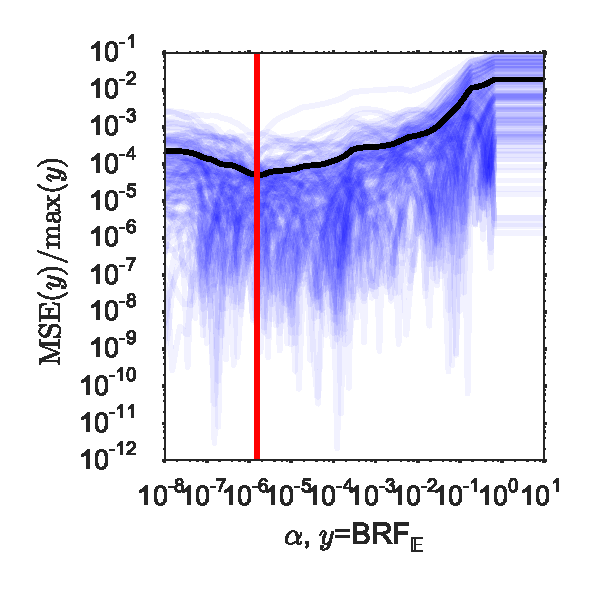
\includegraphics[width=0.32\columnwidth]{Figures/Surrgotes_140-fold/CrossValidation_BRFBM_EFL_M12_E_PCE.pdf}
%\caption{Examples of the cross validation mean squared error (MSE) for the optimization of regularization coefficient. (top row) 20-Fold. (bottom row) 140-fold. (Blue lines) Cross-validation mean square error when each different fold is used as validation dataset. (Black line) Mean of the k-fold cross-validation MSE. (Red line) Selected regularization parameter.}
%\label{fig_20fold}
%\end{centering}
%\end{figure}
%
%
%\section{Legendre polynomials}
%\label{app_leg_poly}
%\small
%
%\eq{\begin{split}
%\phi_{0}(w) & = 1 \\
%\phi_{1}(w) & = w -0.5 \\
%\phi_{2}(w) & = w^2- w+0.166666666667 \\
%\phi_{3}(w) & = w^3+-1.5 w^2+0.6 w-0.05 \\
%\phi_{4}(w) & = w^4-2.0 w^3+1.28571428571 w^2-0.285714285714 w+0.0142857142857\\
%\phi_{5}(w) & = w^5-2.5 w^4+2.22222222222 w^3-0.833333333333 w^2+0.119047619048 w \\
%& -0.00396825396825\\
%\phi_{6}(w) & = w^6-3.0 w^5+3.40909090909 w^4-1.81818181818 w^3+0.454545454545 w^2 \\
%& -0.0454545454545 w +0.00108225108225
%\end{split}
%}{}

%\section{DTU 10 MW RWT surrogates}
%\label{app_surrogates}
%\small
% The resulting polynomial surrogates for the DTU 10 MW RWT are presented in this section. Note that in order to use them it is required to have the Rosenblatt transformation ($R$) and the Logistic transformation ($L$). Additionally, the multi-indexes are given for the Legendre %polynomials on each dimension of $\vw$ with their correspondent coefficient.
%
%% \eq{y = \frac{L^{-1}(\hat{z}(R^{-1}(\vx))) - a_0}{a_1}}{}
%
%\newpage
%
%\begin{table}
%\captionsetup{font=scriptsize}
%\begin{minipage}[!h]{0.25\textwidth}
%\resizebox{0.95\linewidth}{!}{
%\begin{tabular}{|c|cc|}
%\hline
%\hline
%Output &       $a_1$ &       $a_0$ \\
%\hline
%P$_{\expect}$             & $9.5\times10^{-1}$ &  $0$ \\
%CT$_{\expect}$            & $1$ & $-5\times10^{-2}$ \\
%BRF$_{\expect}$ & $2.2\times10^{-2}$ &  $0$ \\
%TBF$_{\expect}$  & $1\times10^{-2}$ &  $0$ \\
%TBS$_{\expect}$  & $1.4\times10^{-2}$ &  $0$ \\
%TTT$_{\expect}$  & $3.3\times10^{-2}$ &  $0$ \\
%TTY$_{\expect}$  & $3.3\times10^{-2}$ &  $0$ \\
%P$_{\std}$             & $22$ &  $1\times10^{-4}$ \\
%CT$_{\std}$            & $5$ &  $1\times10^{-4}$ \\
%BRF$_{\std}$ & $1.7\times10^{-1}$ &  $1\times10^{-4}$ \\
%TBF$_{\std}$  & $2.5\times10^{-2}$ &  $1\times10^{-4}$ \\
%TBS$_{\std}$  & $2.5\times10^{-2}$ &  $1\times10^{-4}$ \\
%TTT$_{\std}$  & $1.7\times10^{-1}$ &  $1\times10^{-4}$ \\
%TTY$_{\std}$  & $1.7\times10^{-1}$ &  $1\times10^{-4}$ \\
%\hline
%\end{tabular}}
%\caption{Logistic transformation constants.}
%%
%\bigskip
%%
%\resizebox{0.95\linewidth}{!}{
%\begin{tabular}{|c|cccc|c|}
%\hline
%\hline
%$j$ &  $l_0$ &  $l_1$ &  $l_2$ &  $l_3$ &  $c_j$ \\
%\hline
%0  &   1 &   0 &   0 &   0 &   17.824827 \\
%1  &   2 &   0 &   0 &   0 &  -78.633549 \\
%2  &   3 &   0 &   0 &   0 &  219.315687 \\
%3  &   4 &   0 &   0 &   0 & -243.351228 \\
%4  &   5 &   0 &   0 &   0 &   90.916652 \\
%5  &   3 &   1 &   0 &   0 &    2.182398 \\
%6  &   0 &   1 &   0 &   0 &   -0.233627 \\
%7  &   1 &   1 &   0 &   0 &    0.674163 \\
%8  &   2 &   1 &   0 &   0 &   -2.880281 \\
%9  &   1 &   2 &   0 &   0 &   -0.065094 \\
%10 &   0 &   2 &   0 &   0 &    0.407897 \\
%11 &   0 &   3 &   0 &   0 &   -0.201789 \\
%12 &   1 &   0 &   1 &   0 &    0.062216 \\
%13 &   2 &   0 &   1 &   0 &    0.419585 \\
%14 &   0 &   1 &   1 &   0 &    0.390699 \\
%15 &   0 &   2 &   1 &   0 &   -0.661779 \\
%16 &   0 &   3 &   1 &   0 &    0.441186 \\
%17 &   0 &   0 &   1 &   0 &   -0.920436 \\
%18 &   1 &   0 &   2 &   0 &   -0.412364 \\
%19 &   0 &   1 &   2 &   0 &    0.107086 \\
%20 &   0 &   0 &   2 &   0 &    1.012321 \\
%21 &   0 &   0 &   3 &   0 &   -0.356882 \\
%22 &   1 &   0 &   0 &   1 &   -0.139125 \\
%23 &   2 &   0 &   0 &   1 &    0.085514 \\
%24 &   1 &   1 &   0 &   1 &    0.123286 \\
%25 &   0 &   1 &   0 &   1 &    0.685970 \\
%26 &   0 &   2 &   0 &   1 &   -0.145333 \\
%27 &   0 &   0 &   1 &   1 &    1.956024 \\
%28 &   1 &   0 &   1 &   1 &   -0.012298 \\
%29 &   2 &   0 &   1 &   1 &   -0.279339 \\
%30 &   0 &   1 &   1 &   1 &   -0.432207 \\
%31 &   0 &   0 &   2 &   1 &   -1.986752 \\
%32 &   0 &   0 &   3 &   1 &    0.134547 \\
%33 &   0 &   0 &   0 &   1 &   -0.453163 \\
%34 &   1 &   0 &   2 &   1 &    0.413360 \\
%35 &   0 &   1 &   0 &   2 &   -0.798297 \\
%36 &   0 &   0 &   1 &   2 &   -1.339587 \\
%37 &   0 &   0 &   0 &   2 &    0.384846 \\
%38 &   0 &   0 &   2 &   2 &    1.779210 \\
%39 &   0 &   1 &   0 &   3 &    0.520667 \\
%40 &   0 &   0 &   1 &   3 &   -0.401148 \\
%41 &   0 &   0 &   0 &   0 &   -3.033096 \\
%42 &   0 &   0 &   0 &   3 &   -0.069222 \\
%\hline
%\end{tabular}}
%\caption{P$_{\expect}$ PCE}
%\end{minipage}%
%%
%\begin{minipage}[!h]{0.25\textwidth}
%\resizebox{0.95\linewidth}{!}{
%\begin{tabular}{|c|cccc|c|}
%\hline
%$j$ &  $l_0$ &  $l_1$ &  $l_2$ &  $l_3$ &  $c_j$ \\
%\hline
%0  &   2 &   0 &   0 &   0 & -134.127728 \\
%1  &   4 &   0 &   0 &   0 & -783.293694 \\
%2  &   5 &   0 &   0 &   0 &  379.323723 \\
%3  &   3 &   1 &   0 &   0 &   92.588283 \\
%4  &   4 &   1 &   0 &   0 &  -54.384443 \\
%5  &   1 &   2 &   0 &   0 &   21.703299 \\
%6  &   0 &   2 &   0 &   0 &  -20.471705 \\
%7  &   0 &   3 &   0 &   0 &   14.812553 \\
%8  &   1 &   3 &   0 &   0 &  -13.073937 \\
%9  &   2 &   0 &   1 &   0 &    9.071876 \\
%10 &   3 &   0 &   1 &   0 &   -6.264682 \\
%11 &   0 &   2 &   1 &   0 &   16.698677 \\
%12 &   0 &   3 &   1 &   0 &  -16.131545 \\
%13 &   0 &   2 &   2 &   0 &    6.641359 \\
%14 &   1 &   0 &   0 &   1 &    8.684951 \\
%15 &   2 &   1 &   0 &   1 &   -0.366464 \\
%16 &   0 &   2 &   0 &   1 &    0.258849 \\
%17 &   1 &   1 &   1 &   1 &   13.799775 \\
%18 &   0 &   0 &   1 &   1 &   10.511176 \\
%19 &   1 &   0 &   1 &   1 &  -36.179227 \\
%20 &   2 &   0 &   1 &   1 &   -0.366464 \\
%21 &   0 &   1 &   1 &   1 &  -30.322117 \\
%22 &   1 &   1 &   2 &   1 &   -1.887029 \\
%23 &   1 &   0 &   0 &   2 &    1.465741 \\
%24 &   1 &   0 &   1 &   2 &    1.603893 \\
%25 &   0 &   1 &   1 &   2 &   32.674897 \\
%26 &   0 &   0 &   1 &   2 &    1.698385 \\
%27 &   0 &   1 &   2 &   2 &  -38.553710 \\
%28 &   0 &   0 &   0 &   2 &    0.061389 \\
%29 &   0 &   0 &   2 &   2 &    9.876207 \\
%30 &   1 &   1 &   0 &   3 &    5.859210 \\
%31 &   0 &   1 &   0 &   3 &    6.117555 \\
%32 &   0 &   0 &   0 &   0 &   -2.352223 \\
%33 &   1 &   0 &   0 &   0 &   16.459288 \\
%34 &   3 &   0 &   0 &   0 &  513.554006 \\
%35 &   0 &   1 &   0 &   0 &    6.573813 \\
%36 &   1 &   1 &   0 &   0 &    4.075511 \\
%37 &   2 &   1 &   0 &   0 &  -47.681732 \\
%38 &   2 &   2 &   0 &   0 &   -1.833545 \\
%39 &   1 &   0 &   1 &   0 &    8.983489 \\
%40 &   0 &   1 &   1 &   0 &   -6.126051 \\
%41 &   1 &   1 &   1 &   0 &   -5.698179 \\
%42 &   0 &   0 &   1 &   0 &   -1.208320 \\
%43 &   2 &   1 &   1 &   0 &    0.650296 \\
%44 &   1 &   0 &   2 &   0 &   -2.751493 \\
%45 &   0 &   1 &   2 &   0 &    4.006299 \\
%46 &   0 &   0 &   2 &   0 &   -0.357406 \\
%47 &   1 &   1 &   2 &   0 &    0.943515 \\
%48 &   1 &   0 &   3 &   0 &   -8.754990 \\
%49 &   0 &   0 &   3 &   0 &    3.099825 \\
%50 &   0 &   1 &   3 &   0 &   -6.986286 \\
%51 &   1 &   1 &   0 &   1 &  -14.029346 \\
%52 &   1 &   2 &   0 &   1 &   -0.517698 \\
%53 &   2 &   1 &   1 &   1 &    0.732929 \\
%54 &   0 &   0 &   2 &   1 &  -15.338654 \\
%55 &   0 &   0 &   0 &   1 &   -2.930817 \\
%56 &   2 &   0 &   0 &   1 &   -0.095476 \\
%57 &   0 &   1 &   0 &   1 &   14.093047 \\
%58 &   1 &   0 &   2 &   1 &   30.012599 \\
%59 &   0 &   1 &   2 &   1 &   30.976181 \\
%60 &   1 &   1 &   0 &   2 &    2.976081 \\
%61 &   0 &   1 &   0 &   2 &  -18.694679 \\
%62 &   1 &   0 &   0 &   3 &   -2.130099 \\
%63 &   0 &   0 &   1 &   3 &   -5.062684 \\
%64 &   0 &   0 &   0 &   3 &    1.364934 \\
%65 &   0 &   0 &   0 &   4 &   -0.753081 \\
%\hline
%\end{tabular}}
%\caption{P$_{\std}$ PCE}
%\end{minipage}%
%%
%\begin{minipage}[!h]{0.25\textwidth}
%\resizebox{0.95\linewidth}{!}{
%\begin{tabular}{|c|cccc|c|}
%\hline
%$j$ &  $l_0$ &  $l_1$ &  $l_2$ &  $l_3$ &  $c_j$ \\
%\hline
%0   &   4 &   0 &   0 &   0 & -827.257448 \\
%1   &   5 &   0 &   0 &   0 &  800.815720 \\
%2   &   6 &   0 &   0 &   0 & -280.606232 \\
%3   &   3 &   1 &   0 &   0 &   17.004492 \\
%4   &   4 &   1 &   0 &   0 &   -8.862149 \\
%5   &   5 &   1 &   0 &   0 &   -0.515021 \\
%6   &   0 &   1 &   0 &   0 &   -2.597773 \\
%7   &   0 &   2 &   0 &   0 &    6.136855 \\
%8   &   0 &   3 &   0 &   0 &   -2.144046 \\
%9   &   0 &   4 &   0 &   0 &   -6.041061 \\
%10  &   1 &   4 &   0 &   0 &   -2.793737 \\
%11  &   0 &   5 &   0 &   0 &    4.207707 \\
%12  &   1 &   0 &   1 &   0 &    2.004547 \\
%13  &   2 &   0 &   1 &   0 &    2.484504 \\
%14  &   3 &   0 &   1 &   0 &    2.370726 \\
%15  &   1 &   1 &   1 &   0 &  -10.335456 \\
%16  &   2 &   1 &   1 &   0 &    3.463070 \\
%17  &   1 &   2 &   1 &   0 &    5.221005 \\
%18  &   2 &   2 &   1 &   0 &   -0.066848 \\
%19  &   1 &   3 &   1 &   0 &   -1.741936 \\
%20  &   3 &   1 &   2 &   0 &   -0.662732 \\
%21  &   0 &   1 &   2 &   0 &  -15.091321 \\
%22  &   0 &   2 &   2 &   0 &   10.824525 \\
%23  &   0 &   3 &   2 &   0 &   -3.766392 \\
%24  &   0 &   0 &   2 &   0 &    9.992672 \\
%25  &   1 &   0 &   3 &   0 &    2.168159 \\
%26  &   1 &   1 &   3 &   0 &   -4.415429 \\
%27  &   0 &   0 &   4 &   0 &    4.140158 \\
%28  &   2 &   0 &   0 &   1 &   -4.118752 \\
%29  &   3 &   0 &   0 &   1 &    3.556601 \\
%30  &   1 &   1 &   0 &   1 &   -3.060339 \\
%31  &   2 &   1 &   0 &   1 &    1.941121 \\
%32  &   0 &   2 &   0 &   1 &  -15.283344 \\
%33  &   0 &   2 &   1 &   1 &    7.305088 \\
%34  &   0 &   0 &   1 &   1 &    5.102290 \\
%35  &   0 &   3 &   1 &   1 &   -2.128947 \\
%36  &   1 &   1 &   2 &   1 &   -0.400943 \\
%37  &   0 &   2 &   2 &   1 &   -4.559060 \\
%38  &   0 &   0 &   2 &   1 &  -15.287274 \\
%39  &   0 &   0 &   4 &   1 &   -7.996038 \\
%40  &   0 &   0 &   0 &   1 &    0.502381 \\
%41  &   0 &   0 &   3 &   1 &   17.420762 \\
%42  &   1 &   0 &   0 &   2 &    6.903704 \\
%43  &   2 &   0 &   0 &   2 &   -0.622189 \\
%44  &   1 &   1 &   0 &   2 &   -1.851140 \\
%45  &   2 &   1 &   0 &   2 &   -1.872743 \\
%46  &   0 &   1 &   1 &   2 &   -1.905920 \\
%47  &   0 &   0 &   1 &   2 &   -0.501649 \\
%48  &   0 &   0 &   2 &   2 &    1.701844 \\
%49  &   2 &   0 &   0 &   3 &    1.505283 \\
%50  &   1 &   1 &   0 &   3 &    2.638588 \\
%51  &   0 &   1 &   0 &   3 &   -2.933920 \\
%52  &   1 &   0 &   1 &   3 &    0.909555 \\
%53  &   0 &   0 &   0 &   4 &   -2.607652 \\
%54  &   0 &   0 &   0 &   0 &    1.886055 \\
%55  &   1 &   0 &   0 &   0 &   -0.923786 \\
%56  &   2 &   0 &   0 &   0 &  -57.123284 \\
%57  &   3 &   0 &   0 &   0 &  360.129037 \\
%58  &   1 &   1 &   0 &   0 &    6.551412 \\
%59  &   2 &   1 &   0 &   0 &  -13.178827 \\
%60  &   1 &   2 &   0 &   0 &  -10.882394 \\
%61  &   2 &   2 &   0 &   0 &    3.012151 \\
%62  &   3 &   2 &   0 &   0 &    2.228364 \\
%63  &   1 &   3 &   0 &   0 &   11.486608 \\
%64  &   2 &   3 &   0 &   0 &   -4.152913 \\
%65  &   4 &   0 &   1 &   0 &   -5.319179 \\
%66  &   3 &   1 &   1 &   0 &    0.662732 \\
%67  &   0 &   1 &   1 &   0 &    8.984505 \\
%68  &   0 &   2 &   1 &   0 &   -9.350190 \\
%69  &   0 &   3 &   1 &   0 &    3.926594 \\
%70  &   0 &   0 &   1 &   0 &   -3.893998 \\
%\end{tabular}}
%\end{minipage}%
%%
%\begin{minipage}[!h]{0.25\textwidth}
%\resizebox{0.95\linewidth}{!}{
%\begin{tabular}{|c|cccc|c|}
%\hline
%$j$ &  $l_0$ &  $l_1$ &  $l_2$ &  $l_3$ &  $c_j$ \\
%\hline
%71  &   1 &   0 &   2 &   0 &   -3.635569 \\
%72  &   2 &   0 &   2 &   0 &   -6.470444 \\
%73  &   3 &   0 &   2 &   0 &    6.374993 \\
%74  &   1 &   1 &   2 &   0 &   15.183301 \\
%75  &   2 &   1 &   2 &   0 &   -3.865114 \\
%76  &   1 &   2 &   2 &   0 &   -3.898113 \\
%77  &   0 &   1 &   3 &   0 &    5.761567 \\
%78  &   0 &   2 &   3 &   0 &   -1.239554 \\
%79  &   0 &   0 &   3 &   0 &  -10.324073 \\
%80  &   1 &   0 &   0 &   1 &    0.319789 \\
%81  &   4 &   0 &   0 &   1 &   -1.499582 \\
%82  &   3 &   1 &   0 &   1 &    0.421050 \\
%83  &   0 &   1 &   0 &   1 &    3.787639 \\
%84  &   1 &   2 &   0 &   1 &    7.826755 \\
%85  &   1 &   3 &   0 &   1 &   -5.966679 \\
%86  &   0 &   3 &   0 &   1 &   16.844501 \\
%87  &   0 &   4 &   0 &   1 &   -5.764745 \\
%88  &   1 &   0 &   1 &   1 &   -2.111665 \\
%89  &   1 &   1 &   1 &   1 &   -0.441080 \\
%90  &   0 &   1 &   1 &   1 &   -5.536196 \\
%91  &   1 &   0 &   2 &   1 &    2.840954 \\
%92  &   0 &   1 &   2 &   1 &   10.786568 \\
%93  &   0 &   1 &   3 &   1 &   -4.628595 \\
%94  &   0 &   1 &   0 &   2 &    3.239449 \\
%95  &   1 &   0 &   1 &   2 &    1.621912 \\
%96  &   0 &   0 &   0 &   2 &   -4.623801 \\
%97  &   0 &   2 &   0 &   2 &   -0.600983 \\
%98  &   1 &   0 &   2 &   2 &   -2.640482 \\
%99  &   0 &   0 &   0 &   3 &    6.205667 \\
%100 &   1 &   0 &   0 &   3 &   -9.102199 \\
%101 &   0 &   2 &   0 &   3 &    0.343968 \\
%102 &   0 &   0 &   1 &   3 &   -1.377748 \\
%103 &   0 &   1 &   1 &   3 &    0.458134 \\
%104 &   0 &   0 &   2 &   3 &    0.040432 \\
%105 &   1 &   0 &   0 &   4 &    2.802899 \\
%106 &   0 &   1 &   0 &   4 &    0.800728 \\
%107 &   0 &   0 &   1 &   4 &    0.696161 \\
%\hline
%\end{tabular}}
%\caption{CT$_{\expect}$ PCE}
%%
%%
%\resizebox{0.95\linewidth}{!}{
%\begin{tabular}{|c|cccc|c|}
%\hline
%$j$ &  $l_0$ &  $l_1$ &  $l_2$ &  $l_3$ &  $c_j$ \\
%\hline
%0  &   1 &   0 &   0 &   0 &  -1.588617 \\
%1  &   2 &   0 &   0 &   0 &   6.960288 \\
%2  &   3 &   0 &   0 &   0 & -13.078366 \\
%3  &   4 &   0 &   0 &   0 &   3.658774 \\
%4  &   0 &   1 &   0 &   0 &   1.268715 \\
%5  &   1 &   1 &   0 &   0 &  -1.307230 \\
%6  &   2 &   1 &   0 &   0 &   0.893358 \\
%7  &   0 &   2 &   0 &   0 &  -1.584460 \\
%8  &   0 &   3 &   0 &   0 &   1.124566 \\
%9  &   1 &   0 &   1 &   0 &   0.096560 \\
%10 &   0 &   1 &   1 &   0 &   0.570601 \\
%11 &   0 &   2 &   1 &   0 &  -0.279196 \\
%12 &   0 &   0 &   1 &   0 &  -0.193227 \\
%13 &   0 &   1 &   2 &   0 &  -0.003906 \\
%14 &   0 &   0 &   2 &   0 &  -0.065941 \\
%15 &   1 &   0 &   0 &   1 &   0.015114 \\
%16 &   2 &   0 &   0 &   1 &  -0.124400 \\
%17 &   0 &   1 &   0 &   1 &   0.231847 \\
%18 &   0 &   0 &   1 &   1 &   0.127705 \\
%19 &   0 &   1 &   1 &   1 &  -0.575000 \\
%20 &   0 &   0 &   2 &   1 &   0.017503 \\
%21 &   0 &   0 &   0 &   1 &   0.037185 \\
%22 &   1 &   0 &   0 &   2 &   0.172970 \\
%23 &   0 &   0 &   1 &   2 &   0.207437 \\
%24 &   0 &   0 &   0 &   2 &  -0.249519 \\
%25 &   0 &   0 &   0 &   0 &  -1.697421 \\
%\hline
%\end{tabular}}
%\caption{CT$_{\std}$ PCE}
%\end{minipage}%
%\end{table}
%%
%\begin{table}
%\captionsetup{font=scriptsize}
%\begin{minipage}[!h]{0.25\textwidth}
%\resizebox{0.95\linewidth}{!}{
%\begin{tabular}{|c|cccc|c|}
%\hline
%$j$ &  $l_0$ &  $l_1$ &  $l_2$ &  $l_3$ &  $c_j$ \\
%\hline
%0  &   4 &   0 &   0 &   0 &  62.694878 \\
%1  &   5 &   0 &   0 &   0 & -62.819279 \\
%2  &   6 &   0 &   0 &   0 &  26.414390 \\
%3  &   3 &   1 &   0 &   0 &   5.073870 \\
%4  &   4 &   1 &   0 &   0 &  -1.010211 \\
%5  &   0 &   1 &   0 &   0 &  -1.232956 \\
%6  &   0 &   2 &   0 &   0 &   3.032444 \\
%7  &   0 &   3 &   0 &   0 &  -1.380097 \\
%8  &   0 &   4 &   0 &   0 &  -2.786755 \\
%9  &   0 &   5 &   0 &   0 &   2.762271 \\
%10 &   1 &   0 &   1 &   0 &   1.593698 \\
%11 &   2 &   0 &   1 &   0 &   1.306560 \\
%12 &   3 &   0 &   1 &   0 &  -1.289262 \\
%13 &   1 &   1 &   1 &   0 &  -1.960311 \\
%14 &   2 &   1 &   1 &   0 &   0.462671 \\
%15 &   1 &   2 &   1 &   0 &   1.284869 \\
%16 &   0 &   1 &   2 &   0 &   2.583334 \\
%17 &   0 &   2 &   2 &   0 &   0.429339 \\
%18 &   0 &   0 &   2 &   0 &  -0.068526 \\
%19 &   1 &   0 &   3 &   0 &  -1.296834 \\
%20 &   2 &   0 &   3 &   0 &   1.644857 \\
%21 &   1 &   1 &   3 &   0 &   1.386674 \\
%22 &   0 &   1 &   4 &   0 &   1.237224 \\
%23 &   0 &   0 &   4 &   0 &  -0.374613 \\
%24 &   2 &   0 &   0 &   1 &  -6.958940 \\
%25 &   3 &   0 &   0 &   1 &   5.302168 \\
%26 &   1 &   1 &   0 &   1 &  -0.544489 \\
%27 &   2 &   1 &   0 &   1 &  -0.096270 \\
%28 &   0 &   2 &   0 &   1 &  -9.320285 \\
%29 &   0 &   0 &   1 &   1 &  -1.387413 \\
%30 &   1 &   1 &   2 &   1 &   2.055372 \\
%31 &   0 &   2 &   2 &   1 &   0.274349 \\
%32 &   0 &   0 &   2 &   1 &   2.407023 \\
%33 &   0 &   0 &   4 &   1 &   1.505527 \\
%34 &   0 &   0 &   0 &   1 &  -0.481728 \\
%35 &   0 &   2 &   1 &   1 &  -0.274349 \\
%36 &   0 &   0 &   3 &   1 &  -3.385077 \\
%37 &   1 &   0 &   0 &   2 &  -2.410568 \\
%38 &   2 &   0 &   0 &   2 &   5.058386 \\
%39 &   3 &   0 &   0 &   2 &  -3.556947 \\
%40 &   1 &   1 &   0 &   2 &   0.679389 \\
%41 &   0 &   1 &   1 &   2 &  -0.627927 \\
%42 &   0 &   0 &   1 &   2 &  -0.107242 \\
%43 &   0 &   0 &   2 &   2 &   2.167533 \\
%44 &   0 &   1 &   0 &   3 &   3.995469 \\
%45 &   1 &   0 &   1 &   3 &   0.335097 \\
%46 &   0 &   0 &   0 &   0 &  -1.621127 \\
%47 &   1 &   0 &   0 &   0 &  -1.236436 \\
%48 &   2 &   0 &   0 &   0 &  16.592903 \\
%49 &   3 &   0 &   0 &   0 & -40.158224 \\
%50 &   1 &   1 &   0 &   0 &   4.115606 \\
%51 &   2 &   1 &   0 &   0 &  -6.819207 \\
%52 &   1 &   2 &   0 &   0 &  -2.273269 \\
%53 &   2 &   2 &   0 &   0 &   1.655239 \\
%54 &   3 &   2 &   0 &   0 &  -0.811717 \\
%55 &   1 &   3 &   0 &   0 &   0.445370 \\
%56 &   4 &   0 &   1 &   0 &   0.589926 \\
%57 &   3 &   1 &   1 &   0 &   0.218822 \\
%58 &   0 &   1 &   1 &   0 &   2.121804 \\
%59 &   0 &   2 &   1 &   0 &  -7.253108 \\
%60 &   0 &   3 &   1 &   0 &   8.743509 \\
%61 &   0 &   4 &   1 &   0 &  -4.116381 \\
%62 &   0 &   0 &   1 &   0 &  -0.998033 \\
%63 &   1 &   0 &   2 &   0 &   1.097308 \\
%64 &   2 &   0 &   2 &   0 &  -2.685648 \\
%65 &   1 &   1 &   2 &   0 &  -1.639455 \\
%66 &   0 &   1 &   3 &   0 &  -3.600087 \\
%67 &   0 &   0 &   3 &   0 &   1.081131 \\
%68 &   1 &   0 &   0 &   1 &   2.818352 \\
%69 &   0 &   1 &   0 &   1 &   4.830761 \\
%70 &   1 &   2 &   0 &   1 &   0.135315 \\
%\end{tabular}}
%\end{minipage}%
%%
%\begin{minipage}[!h]{0.25\textwidth}
%\resizebox{0.95\linewidth}{!}{
%\begin{tabular}{|c|cccc|c|}
%\hline
%$j$ &  $l_0$ &  $l_1$ &  $l_2$ &  $l_3$ &  $c_j$ \\
%\hline
%71 &   0 &   3 &   0 &   1 &   9.122104 \\
%72 &   0 &   4 &   0 &   1 &  -4.121466 \\
%73 &   1 &   0 &   1 &   1 &   0.121521 \\
%74 &   2 &   0 &   1 &   1 &   0.453509 \\
%75 &   1 &   1 &   1 &   1 &  -1.363471 \\
%76 &   0 &   1 &   1 &   1 &   2.146573 \\
%77 &   1 &   0 &   2 &   1 &  -1.027686 \\
%78 &   0 &   1 &   2 &   1 &  -2.642740 \\
%79 &   0 &   1 &   3 &   1 &   0.864604 \\
%80 &   0 &   1 &   0 &   2 &  -6.806370 \\
%81 &   0 &   2 &   0 &   2 &   6.654701 \\
%82 &   1 &   0 &   1 &   2 &   0.234386 \\
%83 &   0 &   0 &   0 &   2 &   0.156466 \\
%84 &   0 &   3 &   0 &   2 &  -0.879173 \\
%85 &   0 &   0 &   0 &   3 &   1.039756 \\
%86 &   1 &   0 &   0 &   3 &  -0.165016 \\
%87 &   0 &   2 &   0 &   3 &  -3.557294 \\
%88 &   0 &   0 &   1 &   3 &  -0.112527 \\
%89 &   0 &   0 &   2 &   3 &  -1.312607 \\
%90 &   0 &   0 &   0 &   4 &  -0.680624 \\
%\hline
%\end{tabular}}
%\caption{BRF$_{\expect}$ PCE}
%%
%%
%\resizebox{0.95\linewidth}{!}{
%\begin{tabular}{|c|cccc|c|}
%\hline
%$j$ &  $l_0$ &  $l_1$ &  $l_2$ &  $l_3$ &  $c_j$ \\
%\hline
%0  &   1 &   0 &   0 &   0 &  5.228706 \\
%1  &   2 &   0 &   0 &   0 & -7.300998 \\
%2  &   3 &   0 &   0 &   0 &  3.523426 \\
%3  &   0 &   1 &   0 &   0 &  0.892945 \\
%4  &   1 &   1 &   0 &   0 & -0.438192 \\
%5  &   0 &   2 &   0 &   0 & -0.313025 \\
%6  &   0 &   3 &   0 &   0 &  0.186111 \\
%7  &   1 &   0 &   1 &   0 &  0.086469 \\
%8  &   0 &   0 &   1 &   0 & -0.202612 \\
%9  &   0 &   0 &   0 &   1 &  0.094581 \\
%10 &   1 &   0 &   0 &   1 & -0.149807 \\
%11 &   0 &   0 &   0 &   0 & -2.244177 \\
%\hline
%\end{tabular}}
%\caption{BRF$_{\std}$ PCE}
%%
%%
%\resizebox{0.95\linewidth}{!}{
%\begin{tabular}{|c|cccc|c|}
%\hline
%$j$ &  $l_0$ &  $l_1$ &  $l_2$ &  $l_3$ &  $c_j$ \\
%\hline
%0  &   1 &   0 &   0 &   0 &   7.492604 \\
%1  &   2 &   0 &   0 &   0 & -30.048707 \\
%2  &   3 &   0 &   0 &   0 &  36.485874 \\
%3  &   4 &   0 &   0 &   0 & -13.644361 \\
%4  &   0 &   1 &   0 &   0 &   2.494525 \\
%5  &   1 &   1 &   0 &   0 &  -2.510374 \\
%6  &   2 &   1 &   0 &   0 &   1.552327 \\
%7  &   1 &   2 &   0 &   0 &  -0.404614 \\
%8  &   0 &   2 &   0 &   0 &  -2.573943 \\
%9  &   0 &   3 &   0 &   0 &   2.080285 \\
%10 &   1 &   0 &   1 &   0 &  -0.000183 \\
%11 &   0 &   1 &   1 &   0 &  -0.031200 \\
%12 &   1 &   1 &   1 &   0 &   0.062401 \\
%13 &   0 &   0 &   1 &   0 &   0.024172 \\
%14 &   1 &   0 &   0 &   1 &  -0.007061 \\
%15 &   1 &   1 &   0 &   1 &   0.363697 \\
%16 &   0 &   1 &   0 &   1 &   0.122950 \\
%17 &   0 &   2 &   0 &   1 &  -0.300063 \\
%18 &   0 &   0 &   1 &   1 &   0.013684 \\
%19 &   0 &   0 &   0 &   1 &  -0.086136 \\
%20 &   1 &   0 &   0 &   2 &  -0.066080 \\
%21 &   0 &   0 &   0 &   2 &   0.029179 \\
%22 &   0 &   0 &   0 &   0 &  -0.720555 \\
%\hline
%\end{tabular}}
%\caption{TBF$_{\expect}$ PCE}
%\end{minipage}%
%%
%\begin{minipage}[!h]{0.25\textwidth}
%\resizebox{0.95\linewidth}{!}{
%\begin{tabular}{|c|cccc|c|}
%\hline
%$j$ &  $l_0$ &  $l_1$ &  $l_2$ &  $l_3$ &  $c_j$ \\
%\hline
%0  &   1 &   0 &   0 &   0 &   3.265241 \\
%1  &   2 &   0 &   0 &   0 &  -8.920657 \\
%2  &   3 &   0 &   0 &   0 & -17.700217 \\
%3  &   4 &   0 &   0 &   0 &  44.803873 \\
%4  &   5 &   0 &   0 &   0 & -22.380164 \\
%5  &   0 &   1 &   0 &   0 &   1.010208 \\
%6  &   1 &   1 &   0 &   0 &  -0.840001 \\
%7  &   2 &   1 &   0 &   0 &   0.216462 \\
%8  &   1 &   2 &   0 &   0 &   0.010459 \\
%9  &   0 &   2 &   0 &   0 &  -1.764214 \\
%10 &   0 &   3 &   0 &   0 &   1.537057 \\
%11 &   1 &   0 &   1 &   0 &   0.187639 \\
%12 &   2 &   0 &   1 &   0 &  -0.218385 \\
%13 &   0 &   1 &   1 &   0 &   1.742232 \\
%14 &   1 &   1 &   1 &   0 &  -0.032924 \\
%15 &   0 &   2 &   1 &   0 &  -1.036063 \\
%16 &   0 &   0 &   1 &   0 &  -0.158630 \\
%17 &   1 &   0 &   2 &   0 &   0.063194 \\
%18 &   0 &   1 &   2 &   0 &  -0.290302 \\
%19 &   0 &   0 &   2 &   0 &  -0.311188 \\
%20 &   0 &   0 &   3 &   0 &   0.012734 \\
%21 &   1 &   0 &   0 &   1 &  -0.721490 \\
%22 &   2 &   0 &   0 &   1 &   1.069445 \\
%23 &   3 &   0 &   0 &   1 &  -0.471808 \\
%24 &   1 &   1 &   0 &   1 &   0.701628 \\
%25 &   2 &   1 &   0 &   1 &  -0.432925 \\
%26 &   0 &   1 &   0 &   1 &   1.772737 \\
%27 &   0 &   2 &   0 &   1 &  -0.906239 \\
%28 &   0 &   0 &   1 &   1 &   0.394469 \\
%29 &   0 &   1 &   1 &   1 &  -4.783365 \\
%30 &   0 &   0 &   2 &   1 &   1.489605 \\
%31 &   0 &   1 &   2 &   1 &   1.288322 \\
%32 &   0 &   0 &   3 &   1 &  -0.484483 \\
%33 &   0 &   0 &   0 &   1 &  -0.529695 \\
%34 &   0 &   2 &   1 &   1 &   1.787082 \\
%35 &   0 &   1 &   0 &   2 &  -0.623935 \\
%36 &   0 &   1 &   1 &   2 &   1.362023 \\
%37 &   0 &   0 &   1 &   2 &  -0.495626 \\
%38 &   0 &   0 &   0 &   2 &   0.592109 \\
%39 &   0 &   0 &   2 &   2 &  -0.893638 \\
%40 &   0 &   0 &   1 &   3 &   0.488628 \\
%41 &   0 &   0 &   0 &   3 &  -0.174881 \\
%42 &   0 &   0 &   0 &   4 &  -0.196241 \\
%43 &   0 &   0 &   0 &   0 &  -1.328826 \\
%\hline
%\end{tabular}}
%\caption{TBF$_{\std}$ PCE}
%%
%%
%\resizebox{0.95\linewidth}{!}{
%\begin{tabular}{|c|cccc|c|}
%\hline
%$j$ &  $l_0$ &  $l_1$ &  $l_2$ &  $l_3$ &  $c_j$ \\
%\hline
%0  &   1 &   0 &   0 &   0 &   17.697877 \\
%1  &   2 &   0 &   0 &   0 &  -78.280278 \\
%2  &   3 &   0 &   0 &   0 &  103.037368 \\
%3  &   4 &   0 &   0 &   0 &  -41.671488 \\
%4  &   1 &   1 &   0 &   0 &   -2.089860 \\
%5  &   2 &   1 &   0 &   0 &    1.038843 \\
%6  &   0 &   1 &   0 &   0 &    2.316537 \\
%7  &   0 &   2 &   0 &   0 &   -2.265180 \\
%8  &   0 &   3 &   0 &   0 &    1.561479 \\
%9  &   1 &   0 &   1 &   0 &    0.774492 \\
%10 &   2 &   0 &   1 &   0 &   -0.476546 \\
%11 &   0 &   0 &   1 &   0 &   -0.261296 \\
%12 &   0 &   0 &   2 &   0 &   -0.055217 \\
%13 &   1 &   0 &   0 &   1 &   -0.118863 \\
%14 &   1 &   1 &   0 &   1 &    0.019715 \\
%15 &   0 &   1 &   0 &   1 &   -0.009858 \\
%16 &   0 &   0 &   0 &   1 &   -0.031550 \\
%17 &   2 &   0 &   0 &   1 &    0.109006 \\
%18 &   0 &   0 &   1 &   1 &    0.044472 \\
%19 &   0 &   0 &   0 &   0 &   -1.161185 \\
%\hline
%\end{tabular}}
%\caption{TBS$_{\expect}$ PCE}
%\end{minipage}%
%%
%\begin{minipage}[!h]{0.25\textwidth}
%\resizebox{0.95\linewidth}{!}{
%\begin{tabular}{|c|cccc|c|}
%\hline
%$j$ &  $l_0$ &  $l_1$ &  $l_2$ &  $l_3$ &  $c_j$ \\
%\hline
%0  &   1 &   0 &   0 &   0 &  12.057073 \\
%1  &   2 &   0 &   0 &   0 & -50.660200 \\
%2  &   3 &   0 &   0 &   0 &  59.790826 \\
%3  &   4 &   0 &   0 &   0 & -21.176517 \\
%4  &   0 &   1 &   0 &   0 &   1.430674 \\
%5  &   1 &   1 &   0 &   0 &  -0.310681 \\
%6  &   2 &   1 &   0 &   0 &  -0.223647 \\
%7  &   0 &   2 &   0 &   0 &  -1.456880 \\
%8  &   0 &   3 &   0 &   0 &   0.942868 \\
%9  &   1 &   0 &   1 &   0 &   0.801769 \\
%10 &   2 &   0 &   1 &   0 &  -0.398060 \\
%11 &   0 &   1 &   1 &   0 &  -0.634770 \\
%12 &   0 &   2 &   1 &   0 &  -0.185424 \\
%13 &   0 &   0 &   1 &   0 &   0.336571 \\
%14 &   0 &   1 &   2 &   0 &   1.058729 \\
%15 &   0 &   0 &   2 &   0 &  -0.824320 \\
%16 &   1 &   0 &   0 &   1 &   0.000604 \\
%17 &   0 &   1 &   0 &   1 &   0.356178 \\
%18 &   0 &   0 &   1 &   1 &  -0.309698 \\
%19 &   0 &   1 &   1 &   1 &  -0.539143 \\
%20 &   0 &   0 &   2 &   1 &   0.551080 \\
%21 &   0 &   0 &   0 &   1 &   0.175367 \\
%22 &   0 &   0 &   0 &   2 &  -0.261448 \\
%23 &   0 &   0 &   0 &   0 &  -2.003581 \\
%\hline
%\end{tabular}}
%\caption{TBS$_{\std}$ PCE}
%%
%%
%\resizebox{0.95\linewidth}{!}{
%\begin{tabular}{|c|cccc|c|}
%\hline
%$j$ &  $l_0$ &  $l_1$ &  $l_2$ &  $l_3$ &  $c_j$ \\
%\hline
%0  &   1 &   0 &   0 &   0 &   2.178824 \\
%1  &   2 &   0 &   0 &   0 &  -7.768412 \\
%2  &   4 &   0 &   0 &   0 & -50.663690 \\
%3  &   5 &   0 &   0 &   0 &  23.926302 \\
%4  &   3 &   1 &   0 &   0 &  -0.565525 \\
%5  &   4 &   1 &   0 &   0 &   0.439384 \\
%6  &   1 &   2 &   0 &   0 &  -0.705630 \\
%7  &   0 &   2 &   0 &   0 &  -7.614740 \\
%8  &   0 &   3 &   0 &   0 &  16.671007 \\
%9  &   1 &   4 &   0 &   0 &   0.087152 \\
%10 &   0 &   4 &   0 &   0 & -17.206161 \\
%11 &   0 &   5 &   0 &   0 &   6.856903 \\
%12 &   2 &   0 &   1 &   0 &   0.225416 \\
%13 &   3 &   0 &   1 &   0 &  -0.070966 \\
%14 &   1 &   2 &   1 &   0 &   0.378023 \\
%15 &   0 &   2 &   1 &   0 &  -0.266672 \\
%16 &   2 &   0 &   2 &   0 &  -0.213454 \\
%17 &   0 &   0 &   2 &   0 &  -0.438691 \\
%18 &   0 &   2 &   2 &   0 &   0.118678 \\
%19 &   3 &   0 &   0 &   1 &  -0.262115 \\
%20 &   2 &   1 &   0 &   1 &   0.659012 \\
%21 &   0 &   2 &   0 &   1 &  -0.175919 \\
%22 &   0 &   3 &   0 &   1 &   0.269048 \\
%23 &   1 &   1 &   1 &   1 &  -3.690833 \\
%24 &   0 &   0 &   1 &   1 &  -1.195231 \\
%25 &   1 &   0 &   1 &   1 &   2.176106 \\
%26 &   0 &   1 &   1 &   1 &   2.068393 \\
%27 &   1 &   1 &   2 &   1 &   2.963454 \\
%28 &   0 &   0 &   2 &   1 &   0.897428 \\
%29 &   1 &   0 &   0 &   2 &  -0.227329 \\
%30 &   2 &   1 &   0 &   2 &  -0.628790 \\
%31 &   1 &   0 &   1 &   2 &   0.111038 \\
%32 &   0 &   1 &   1 &   2 &  -0.318772 \\
%33 &   0 &   0 &   1 &   2 &   0.024201 \\
%34 &   0 &   0 &   0 &   2 &  -0.643182 \\
%35 &   1 &   0 &   0 &   3 &  -0.313404 \\
%36 &   0 &   1 &   0 &   3 &  -0.106257 \\
%37 &   0 &   0 &   1 &   3 &  -0.053350 \\
%38 &   0 &   0 &   0 &   0 &  -2.444218 \\
%39 &   3 &   0 &   0 &   0 &  34.800840 \\
%40 &   0 &   1 &   0 &   0 &   2.392428 \\
%\end{tabular}}
%\end{minipage}%
%\end{table}
%%
%\begin{table}
%\captionsetup{font=scriptsize}
%\begin{minipage}[!h]{0.25\textwidth}
%\resizebox{0.95\linewidth}{!}{
%\begin{tabular}{|c|cccc|c|}
%\hline
%$j$ &  $l_0$ &  $l_1$ &  $l_2$ &  $l_3$ &  $c_j$ \\
%\hline
%41 &   1 &   1 &   0 &   0 &  -0.090892 \\
%42 &   2 &   1 &   0 &   0 &  -0.016337 \\
%43 &   2 &   2 &   0 &   0 &   0.182759 \\
%44 &   1 &   3 &   0 &   0 &   0.146621 \\
%45 &   1 &   0 &   1 &   0 &  -0.918469 \\
%46 &   0 &   1 &   1 &   0 &  -0.834861 \\
%47 &   1 &   1 &   1 &   0 &   1.160205 \\
%48 &   0 &   0 &   1 &   0 &   0.517650 \\
%49 &   2 &   1 &   1 &   0 &   0.077137 \\
%50 &   1 &   0 &   2 &   0 &   0.807578 \\
%51 &   0 &   1 &   2 &   0 &   1.271804 \\
%52 &   1 &   1 &   2 &   0 &  -1.227169 \\
%53 &   0 &   0 &   3 &   0 &  -0.085267 \\
%54 &   0 &   1 &   3 &   0 &  -0.748541 \\
%55 &   0 &   0 &   4 &   0 &   0.163983 \\
%56 &   0 &   1 &   4 &   0 &   0.160297 \\
%57 &   0 &   0 &   0 &   1 &   0.502672 \\
%58 &   1 &   0 &   0 &   1 &  -0.175084 \\
%59 &   2 &   0 &   0 &   1 &  -0.231019 \\
%60 &   1 &   1 &   0 &   1 &   0.057341 \\
%61 &   0 &   1 &   0 &   1 &  -0.396614 \\
%62 &   1 &   2 &   0 &   1 &   0.088325 \\
%63 &   0 &   2 &   1 &   1 &  -0.204892 \\
%64 &   1 &   0 &   2 &   1 &  -1.828650 \\
%65 &   0 &   1 &   2 &   1 &  -1.281523 \\
%66 &   2 &   0 &   0 &   2 &   0.596522 \\
%67 &   1 &   1 &   0 &   2 &   0.685547 \\
%68 &   0 &   1 &   0 &   2 &   0.218409 \\
%69 &   0 &   2 &   0 &   2 &  -0.211704 \\
%70 &   0 &   1 &   1 &   3 &   0.212514 \\
%71 &   0 &   0 &   0 &   3 &   0.744282 \\
%72 &   0 &   0 &   0 &   4 &  -0.238186 \\
%\hline
%\end{tabular}}
%\caption{TTT$_{\expect}$ PCE}
%%
%%
%\resizebox{0.95\linewidth}{!}{
%\begin{tabular}{|c|cccc|c|}
%\hline
%$j$ &  $l_0$ &  $l_1$ &  $l_2$ &  $l_3$ &  $c_j$ \\
%\hline
%0  &   4 &   0 &   0 &   0 & -296.844378 \\
%1  &   5 &   0 &   0 &   0 &  232.852778 \\
%2  &   6 &   0 &   0 &   0 &  -68.220514 \\
%3  &   3 &   1 &   0 &   0 &   -3.652611 \\
%4  &   4 &   1 &   0 &   0 &    1.308967 \\
%5  &   0 &   1 &   0 &   0 &    3.367015 \\
%6  &   0 &   2 &   0 &   0 &   -7.865412 \\
%7  &   0 &   3 &   0 &   0 &   14.720705 \\
%8  &   0 &   4 &   0 &   0 &  -13.465583 \\
%9  &   1 &   4 &   0 &   0 &    2.100920 \\
%10 &   0 &   5 &   0 &   0 &    4.661932 \\
%11 &   1 &   0 &   1 &   0 &   -5.645130 \\
%12 &   2 &   0 &   1 &   0 &    6.548212 \\
%13 &   3 &   0 &   1 &   0 &   -3.027013 \\
%14 &   1 &   1 &   1 &   0 &    4.614054 \\
%15 &   2 &   1 &   1 &   0 &   -3.818255 \\
%16 &   1 &   2 &   1 &   0 &    0.393950 \\
%17 &   0 &   1 &   2 &   0 &    1.240415 \\
%18 &   0 &   2 &   2 &   0 &    0.028452 \\
%19 &   0 &   0 &   2 &   0 &   -0.378514 \\
%20 &   1 &   0 &   3 &   0 &   -0.565743 \\
%21 &   2 &   0 &   3 &   0 &    0.506597 \\
%22 &   1 &   1 &   3 &   0 &    0.021144 \\
%23 &   0 &   0 &   4 &   0 &    0.647403 \\
%24 &   2 &   0 &   0 &   1 &   -0.384179 \\
%25 &   3 &   0 &   0 &   1 &    4.306313 \\
%26 &   1 &   1 &   0 &   1 &    4.567803 \\
%27 &   2 &   1 &   0 &   1 &   -1.656415 \\
%28 &   0 &   2 &   0 &   1 &   -0.809267 \\
%29 &   0 &   2 &   1 &   1 &    2.049309 \\
%30 &   0 &   0 &   2 &   1 &   -0.738809 \\
%\end{tabular}}
%\end{minipage}%
%%
%\begin{minipage}[!h]{0.25\textwidth}
%\resizebox{0.95\linewidth}{!}{
%\begin{tabular}{|c|cccc|c|}
%\hline
%$j$ &  $l_0$ &  $l_1$ &  $l_2$ &  $l_3$ &  $c_j$ \\
%\hline
%31 &   0 &   0 &   0 &   1 &    1.764704 \\
%32 &   0 &   0 &   1 &   1 &   -1.301562 \\
%33 &   0 &   3 &   1 &   1 &   -1.403386 \\
%34 &   1 &   1 &   2 &   1 &    1.639571 \\
%35 &   0 &   0 &   3 &   1 &    0.668712 \\
%36 &   1 &   0 &   0 &   2 &    6.707797 \\
%37 &   2 &   0 &   0 &   2 &   -2.833838 \\
%38 &   3 &   0 &   0 &   2 &   -0.204807 \\
%39 &   1 &   1 &   0 &   2 &   -1.884884 \\
%40 &   0 &   1 &   1 &   2 &    2.118892 \\
%41 &   0 &   0 &   1 &   2 &    0.781327 \\
%42 &   0 &   1 &   2 &   2 &   -2.068479 \\
%43 &   0 &   0 &   2 &   2 &    0.856648 \\
%44 &   2 &   0 &   0 &   3 &    2.071349 \\
%45 &   1 &   1 &   0 &   3 &    1.072299 \\
%46 &   0 &   1 &   0 &   3 &    0.171253 \\
%47 &   1 &   0 &   1 &   3 &    1.986781 \\
%48 &   0 &   0 &   0 &   4 &   -1.504521 \\
%49 &   0 &   0 &   1 &   4 &    0.100263 \\
%50 &   0 &   0 &   0 &   0 &   -3.144030 \\
%51 &   1 &   0 &   0 &   0 &    6.599387 \\
%52 &   2 &   0 &   0 &   0 &  -45.341285 \\
%53 &   3 &   0 &   0 &   0 &  172.955502 \\
%54 &   1 &   1 &   0 &   0 &   -4.733793 \\
%55 &   2 &   1 &   0 &   0 &    4.476663 \\
%56 &   1 &   2 &   0 &   0 &    4.081142 \\
%57 &   2 &   2 &   0 &   0 &   -0.812257 \\
%58 &   3 &   2 &   0 &   0 &    0.246905 \\
%59 &   1 &   3 &   0 &   0 &   -4.342735 \\
%60 &   3 &   1 &   1 &   0 &    1.005514 \\
%61 &   0 &   1 &   1 &   0 &   -0.858742 \\
%62 &   0 &   2 &   1 &   0 &   -1.332080 \\
%63 &   0 &   3 &   1 &   0 &    0.521297 \\
%64 &   0 &   4 &   1 &   0 &    0.142228 \\
%65 &   0 &   0 &   1 &   0 &    1.247676 \\
%66 &   1 &   0 &   2 &   0 &    4.465628 \\
%67 &   2 &   0 &   2 &   0 &   -5.263632 \\
%68 &   3 &   0 &   2 &   0 &    2.304830 \\
%69 &   1 &   1 &   2 &   0 &   -1.701401 \\
%70 &   2 &   1 &   2 &   0 &    0.849900 \\
%71 &   0 &   1 &   3 &   0 &   -0.772282 \\
%72 &   0 &   0 &   3 &   0 &   -0.931977 \\
%73 &   1 &   0 &   4 &   0 &   -0.164284 \\
%74 &   1 &   0 &   0 &   1 &   -4.312543 \\
%75 &   4 &   0 &   0 &   1 &   -2.452739 \\
%76 &   3 &   1 &   0 &   1 &    0.570028 \\
%77 &   0 &   1 &   0 &   1 &   -1.126498 \\
%78 &   1 &   2 &   0 &   1 &   -1.177847 \\
%79 &   0 &   3 &   0 &   1 &    1.278235 \\
%80 &   1 &   0 &   1 &   1 &    6.296783 \\
%81 &   2 &   0 &   1 &   1 &   -1.522185 \\
%82 &   1 &   1 &   1 &   1 &   -5.723955 \\
%83 &   0 &   1 &   1 &   1 &   -0.900966 \\
%84 &   2 &   1 &   1 &   1 &    1.808171 \\
%85 &   1 &   0 &   2 &   1 &   -2.307984 \\
%86 &   0 &   1 &   2 &   1 &    1.433679 \\
%87 &   0 &   1 &   0 &   2 &    0.185031 \\
%88 &   0 &   2 &   0 &   2 &    0.144689 \\
%89 &   1 &   0 &   1 &   2 &   -3.835372 \\
%90 &   0 &   0 &   0 &   2 &   -2.831547 \\
%91 &   2 &   0 &   1 &   2 &    0.278039 \\
%92 &   1 &   1 &   1 &   2 &    0.443955 \\
%93 &   1 &   0 &   2 &   2 &    0.355184 \\
%94 &   0 &   0 &   0 &   3 &    2.855987 \\
%95 &   1 &   0 &   0 &   3 &   -4.437864 \\
%96 &   0 &   2 &   0 &   3 &   -0.560837 \\
%97 &   0 &   0 &   1 &   3 &   -1.193917 \\
%98 &   0 &   0 &   0 &   5 &    0.568050 \\
%\hline
%\end{tabular}}
%\caption{TTT$_{\std}$ PCE}
%\end{minipage}%
%%
%%
%\begin{minipage}[!h]{0.25\textwidth}
%\resizebox{0.95\linewidth}{!}{
%\begin{tabular}{|c|cccc|c|}
%\hline
%$j$ &  $l_0$ &  $l_1$ &  $l_2$ &  $l_3$ &  $c_j$ \\
%\hline
%0  &   4 &   0 &   0 &   0 & -26.193393 \\
%1  &   5 &   0 &   0 &   0 &  14.668184 \\
%2  &   3 &   1 &   0 &   0 &   0.701493 \\
%3  &   0 &   1 &   0 &   0 &   2.398323 \\
%4  &   0 &   2 &   0 &   0 &  -8.320975 \\
%5  &   0 &   3 &   0 &   0 &  17.868359 \\
%6  &   0 &   4 &   0 &   0 & -18.466403 \\
%7  &   0 &   5 &   0 &   0 &   7.456144 \\
%8  &   1 &   0 &   1 &   0 &  -0.984337 \\
%9  &   2 &   0 &   1 &   0 &   1.137439 \\
%10 &   3 &   0 &   1 &   0 &  -0.836179 \\
%11 &   1 &   1 &   1 &   0 &   1.129655 \\
%12 &   2 &   1 &   1 &   0 &   0.447307 \\
%13 &   1 &   2 &   1 &   0 &  -1.247363 \\
%14 &   1 &   3 &   1 &   0 &   1.085180 \\
%15 &   0 &   1 &   2 &   0 &   2.010482 \\
%16 &   0 &   2 &   2 &   0 &  -0.425747 \\
%17 &   0 &   0 &   2 &   0 &  -0.375596 \\
%18 &   1 &   0 &   3 &   0 &  -0.652325 \\
%19 &   2 &   0 &   3 &   0 &   0.377566 \\
%20 &   1 &   1 &   3 &   0 &   0.964014 \\
%21 &   0 &   1 &   4 &   0 &   0.323884 \\
%22 &   0 &   0 &   4 &   0 &   0.340476 \\
%23 &   3 &   0 &   0 &   1 &   0.944969 \\
%24 &   1 &   1 &   0 &   1 &  -0.055687 \\
%25 &   2 &   1 &   0 &   1 &   0.416371 \\
%26 &   0 &   2 &   0 &   1 &  -0.360622 \\
%27 &   0 &   2 &   1 &   1 &  -0.989066 \\
%28 &   0 &   0 &   1 &   1 &  -0.138981 \\
%29 &   0 &   2 &   2 &   1 &   1.036203 \\
%30 &   0 &   0 &   2 &   1 &   0.156162 \\
%31 &   0 &   0 &   0 &   1 &  -0.022514 \\
%32 &   2 &   0 &   0 &   1 &  -1.831250 \\
%33 &   0 &   3 &   1 &   1 &  -0.138527 \\
%34 &   1 &   1 &   2 &   1 &   2.149090 \\
%35 &   1 &   0 &   0 &   2 &  -0.541005 \\
%36 &   2 &   0 &   0 &   2 &   1.679933 \\
%37 &   3 &   0 &   0 &   2 &  -1.062047 \\
%38 &   1 &   1 &   0 &   2 &   0.297611 \\
%39 &   0 &   1 &   1 &   2 &   0.512779 \\
%40 &   0 &   0 &   1 &   2 &  -0.730130 \\
%41 &   0 &   1 &   2 &   2 &  -0.512779 \\
%42 &   0 &   0 &   2 &   2 &   0.847942 \\
%43 &   1 &   1 &   0 &   3 &  -0.017688 \\
%44 &   0 &   1 &   0 &   3 &   0.364082 \\
%45 &   0 &   0 &   0 &   4 &  -0.352532 \\
%46 &   0 &   0 &   0 &   0 &  -2.426329 \\
%47 &   1 &   0 &   0 &   0 &   1.592834 \\
%48 &   2 &   0 &   0 &   0 &   0.211332 \\
%49 &   3 &   0 &   0 &   0 &  12.180566 \\
%50 &   1 &   1 &   0 &   0 &  -0.330041 \\
%51 &   2 &   1 &   0 &   0 &  -0.556099 \\
%52 &   1 &   2 &   0 &   0 &   1.550094 \\
%53 &   2 &   2 &   0 &   0 &  -1.490756 \\
%54 &   1 &   3 &   0 &   0 &  -1.257182 \\
%55 &   2 &   3 &   0 &   0 &   1.125366 \\
%56 &   4 &   0 &   1 &   0 &   0.274710 \\
%57 &   0 &   1 &   1 &   0 &  -0.923899 \\
%58 &   0 &   2 &   1 &   0 &   0.243594 \\
%59 &   0 &   3 &   1 &   0 &   0.347007 \\
%60 &   0 &   4 &   1 &   0 &  -0.347915 \\
%61 &   0 &   0 &   1 &   0 &   0.222753 \\
%62 &   1 &   0 &   2 &   0 &   1.579883 \\
%63 &   2 &   0 &   2 &   0 &  -0.905071 \\
%64 &   1 &   1 &   2 &   0 &  -2.094878 \\
%65 &   0 &   1 &   3 &   0 &  -1.296330
%\end{tabular}}
%\end{minipage}%
%%
%\begin{minipage}[!h]{0.25\textwidth}
%\resizebox{0.95\linewidth}{!}{
%\begin{tabular}{|c|cccc|c|}
%\hline
%$j$ &  $l_0$ &  $l_1$ &  $l_2$ &  $l_3$ &  $c_j$ \\
%\hline
%66 &   0 &   0 &   3 &   0 &  -0.117356 \\
%67 &   0 &   0 &   5 &   0 &  -0.101116 \\
%68 &   1 &   0 &   0 &   1 &   0.733840 \\
%69 &   0 &   1 &   0 &   1 &   0.127638 \\
%70 &   1 &   2 &   0 &   1 &  -0.207187 \\
%71 &   0 &   3 &   0 &   1 &   0.386181 \\
%72 &   1 &   0 &   1 &   1 &   0.728265 \\
%73 &   2 &   0 &   1 &   1 &   0.416371 \\
%74 &   1 &   1 &   1 &   1 &  -1.760808 \\
%75 &   0 &   1 &   1 &   1 &   1.475358 \\
%76 &   2 &   1 &   1 &   1 &  -0.832742 \\
%77 &   1 &   2 &   1 &   1 &   0.321306 \\
%78 &   1 &   0 &   2 &   1 &  -1.284754 \\
%79 &   0 &   1 &   2 &   1 &  -1.475597 \\
%80 &   0 &   1 &   0 &   2 &  -0.530989 \\
%81 &   1 &   0 &   1 &   2 &   0.272549 \\
%82 &   0 &   0 &   0 &   2 &  -0.255484 \\
%83 &   0 &   2 &   0 &   2 &   0.297006 \\
%84 &   0 &   0 &   0 &   3 &   0.726089 \\
%85 &   1 &   0 &   0 &   3 &  -0.351055 \\
%86 &   0 &   2 &   0 &   3 &  -0.366531 \\
%87 &   0 &   0 &   1 &   3 &   0.034960 \\
%88 &   0 &   0 &   2 &   3 &  -0.180979 \\
%\hline
%\end{tabular}}
%\caption{TTY$_{\expect}$ PCE}
%%
%%
%\resizebox{0.95\linewidth}{!}{
%\begin{tabular}{|c|cccc|c|}
%\hline
%$j$ &  $l_0$ &  $l_1$ &  $l_2$ &  $l_3$ &  $c_j$ \\
%\hline
%0  &   1 &   0 &   0 &   0 &  -0.110113 \\
%1  &   2 &   0 &   0 &   0 &   8.259241 \\
%2  &   3 &   0 &   0 &   0 & -13.260383 \\
%3  &   4 &   0 &   0 &   0 &   6.281290 \\
%4  &   0 &   1 &   0 &   0 &   1.221769 \\
%5  &   1 &   1 &   0 &   0 &  -0.130064 \\
%6  &   2 &   1 &   0 &   0 &  -0.260403 \\
%7  &   0 &   2 &   0 &   0 &  -1.677454 \\
%8  &   0 &   3 &   0 &   0 &   1.212444 \\
%9  &   1 &   0 &   1 &   0 &   0.021723 \\
%10 &   0 &   1 &   1 &   0 &   0.101919 \\
%11 &   0 &   2 &   1 &   0 &  -0.092649 \\
%12 &   0 &   0 &   1 &   0 &  -0.011172 \\
%13 &   1 &   0 &   2 &   0 &  -0.024707 \\
%14 &   0 &   0 &   2 &   0 &  -0.025082 \\
%15 &   1 &   0 &   0 &   1 &   0.084859 \\
%16 &   2 &   0 &   0 &   1 &  -0.068179 \\
%17 &   1 &   1 &   0 &   1 &   0.002320 \\
%18 &   0 &   1 &   0 &   1 &   0.241057 \\
%19 &   0 &   2 &   0 &   1 &  -0.189773 \\
%20 &   0 &   0 &   1 &   1 &  -0.030629 \\
%21 &   1 &   0 &   1 &   1 &   0.005969 \\
%22 &   0 &   0 &   2 &   1 &   0.012245 \\
%23 &   0 &   0 &   0 &   1 &   0.054018 \\
%24 &   1 &   0 &   0 &   2 &  -0.059899 \\
%25 &   0 &   1 &   0 &   2 &  -0.021154 \\
%26 &   0 &   0 &   1 &   2 &   0.025697 \\
%27 &   0 &   0 &   0 &   2 &  -0.089572 \\
%28 &   0 &   0 &   0 &   0 &  -2.558245 \\
%\hline
%\end{tabular}}
%\caption{TTY$_{\std}$ PCE}
%\end{minipage}%
%\end{table}

\end{document}
\endinput
%%
%% End of file `elsarticle-template-num.tex'.
